% Options for packages loaded elsewhere
\PassOptionsToPackage{unicode}{hyperref}
\PassOptionsToPackage{hyphens}{url}
%
\documentclass[
]{book}
\usepackage{amsmath,amssymb}
\usepackage{iftex}
\ifPDFTeX
  \usepackage[T1]{fontenc}
  \usepackage[utf8]{inputenc}
  \usepackage{textcomp} % provide euro and other symbols
\else % if luatex or xetex
  \usepackage{unicode-math} % this also loads fontspec
  \defaultfontfeatures{Scale=MatchLowercase}
  \defaultfontfeatures[\rmfamily]{Ligatures=TeX,Scale=1}
\fi
\usepackage{lmodern}
\ifPDFTeX\else
  % xetex/luatex font selection
\fi
% Use upquote if available, for straight quotes in verbatim environments
\IfFileExists{upquote.sty}{\usepackage{upquote}}{}
\IfFileExists{microtype.sty}{% use microtype if available
  \usepackage[]{microtype}
  \UseMicrotypeSet[protrusion]{basicmath} % disable protrusion for tt fonts
}{}
\makeatletter
\@ifundefined{KOMAClassName}{% if non-KOMA class
  \IfFileExists{parskip.sty}{%
    \usepackage{parskip}
  }{% else
    \setlength{\parindent}{0pt}
    \setlength{\parskip}{6pt plus 2pt minus 1pt}}
}{% if KOMA class
  \KOMAoptions{parskip=half}}
\makeatother
\usepackage{xcolor}
\usepackage{color}
\usepackage{fancyvrb}
\newcommand{\VerbBar}{|}
\newcommand{\VERB}{\Verb[commandchars=\\\{\}]}
\DefineVerbatimEnvironment{Highlighting}{Verbatim}{commandchars=\\\{\}}
% Add ',fontsize=\small' for more characters per line
\usepackage{framed}
\definecolor{shadecolor}{RGB}{248,248,248}
\newenvironment{Shaded}{\begin{snugshade}}{\end{snugshade}}
\newcommand{\AlertTok}[1]{\textcolor[rgb]{0.94,0.16,0.16}{#1}}
\newcommand{\AnnotationTok}[1]{\textcolor[rgb]{0.56,0.35,0.01}{\textbf{\textit{#1}}}}
\newcommand{\AttributeTok}[1]{\textcolor[rgb]{0.13,0.29,0.53}{#1}}
\newcommand{\BaseNTok}[1]{\textcolor[rgb]{0.00,0.00,0.81}{#1}}
\newcommand{\BuiltInTok}[1]{#1}
\newcommand{\CharTok}[1]{\textcolor[rgb]{0.31,0.60,0.02}{#1}}
\newcommand{\CommentTok}[1]{\textcolor[rgb]{0.56,0.35,0.01}{\textit{#1}}}
\newcommand{\CommentVarTok}[1]{\textcolor[rgb]{0.56,0.35,0.01}{\textbf{\textit{#1}}}}
\newcommand{\ConstantTok}[1]{\textcolor[rgb]{0.56,0.35,0.01}{#1}}
\newcommand{\ControlFlowTok}[1]{\textcolor[rgb]{0.13,0.29,0.53}{\textbf{#1}}}
\newcommand{\DataTypeTok}[1]{\textcolor[rgb]{0.13,0.29,0.53}{#1}}
\newcommand{\DecValTok}[1]{\textcolor[rgb]{0.00,0.00,0.81}{#1}}
\newcommand{\DocumentationTok}[1]{\textcolor[rgb]{0.56,0.35,0.01}{\textbf{\textit{#1}}}}
\newcommand{\ErrorTok}[1]{\textcolor[rgb]{0.64,0.00,0.00}{\textbf{#1}}}
\newcommand{\ExtensionTok}[1]{#1}
\newcommand{\FloatTok}[1]{\textcolor[rgb]{0.00,0.00,0.81}{#1}}
\newcommand{\FunctionTok}[1]{\textcolor[rgb]{0.13,0.29,0.53}{\textbf{#1}}}
\newcommand{\ImportTok}[1]{#1}
\newcommand{\InformationTok}[1]{\textcolor[rgb]{0.56,0.35,0.01}{\textbf{\textit{#1}}}}
\newcommand{\KeywordTok}[1]{\textcolor[rgb]{0.13,0.29,0.53}{\textbf{#1}}}
\newcommand{\NormalTok}[1]{#1}
\newcommand{\OperatorTok}[1]{\textcolor[rgb]{0.81,0.36,0.00}{\textbf{#1}}}
\newcommand{\OtherTok}[1]{\textcolor[rgb]{0.56,0.35,0.01}{#1}}
\newcommand{\PreprocessorTok}[1]{\textcolor[rgb]{0.56,0.35,0.01}{\textit{#1}}}
\newcommand{\RegionMarkerTok}[1]{#1}
\newcommand{\SpecialCharTok}[1]{\textcolor[rgb]{0.81,0.36,0.00}{\textbf{#1}}}
\newcommand{\SpecialStringTok}[1]{\textcolor[rgb]{0.31,0.60,0.02}{#1}}
\newcommand{\StringTok}[1]{\textcolor[rgb]{0.31,0.60,0.02}{#1}}
\newcommand{\VariableTok}[1]{\textcolor[rgb]{0.00,0.00,0.00}{#1}}
\newcommand{\VerbatimStringTok}[1]{\textcolor[rgb]{0.31,0.60,0.02}{#1}}
\newcommand{\WarningTok}[1]{\textcolor[rgb]{0.56,0.35,0.01}{\textbf{\textit{#1}}}}
\usepackage{longtable,booktabs,array}
\usepackage{calc} % for calculating minipage widths
% Correct order of tables after \paragraph or \subparagraph
\usepackage{etoolbox}
\makeatletter
\patchcmd\longtable{\par}{\if@noskipsec\mbox{}\fi\par}{}{}
\makeatother
% Allow footnotes in longtable head/foot
\IfFileExists{footnotehyper.sty}{\usepackage{footnotehyper}}{\usepackage{footnote}}
\makesavenoteenv{longtable}
\usepackage{graphicx}
\makeatletter
\def\maxwidth{\ifdim\Gin@nat@width>\linewidth\linewidth\else\Gin@nat@width\fi}
\def\maxheight{\ifdim\Gin@nat@height>\textheight\textheight\else\Gin@nat@height\fi}
\makeatother
% Scale images if necessary, so that they will not overflow the page
% margins by default, and it is still possible to overwrite the defaults
% using explicit options in \includegraphics[width, height, ...]{}
\setkeys{Gin}{width=\maxwidth,height=\maxheight,keepaspectratio}
% Set default figure placement to htbp
\makeatletter
\def\fps@figure{htbp}
\makeatother
\setlength{\emergencystretch}{3em} % prevent overfull lines
\providecommand{\tightlist}{%
  \setlength{\itemsep}{0pt}\setlength{\parskip}{0pt}}
\setcounter{secnumdepth}{5}
\usepackage{booktabs}
\usepackage{amsthm}
\usepackage[pagebackref=false,breaklinks=true,letterpaper=true,colorlinks,bookmarks=false]{hyperref}
\usepackage{tcolorbox}
\usepackage{color}
\usepackage{framed}
\setlength{\fboxsep}{.8em}
\makeatletter
\def\thm@space@setup{%
  \thm@preskip=8pt plus 2pt minus 4pt
  \thm@postskip=\thm@preskip
}
\makeatother

% \newcommand{\calM}{\mathcal{M}}


\newtcolorbox{examplebox}{
  colback=green,
  colframe=orange,
  coltext=black,
  boxsep=5pt,
  arc=4pt}

\newtcolorbox{theorembox}{
  colback=green,
  colframe=green,
  coltext=black,
  boxsep=5pt,
  arc=4pt}

\newtcolorbox{definitionbox}{
colback=white,
colframe=green,
coltext=black,
boxsep=5pt,
arc=4pt}
\ifLuaTeX
  \usepackage{selnolig}  % disable illegal ligatures
\fi
\usepackage[]{natbib}
\bibliographystyle{apalike}
\usepackage{bookmark}
\IfFileExists{xurl.sty}{\usepackage{xurl}}{} % add URL line breaks if available
\urlstyle{same}
\hypersetup{
  pdftitle={Optimal Control and Reinforcement Learning},
  pdfauthor={Heng Yang},
  hidelinks,
  pdfcreator={LaTeX via pandoc}}

\title{Optimal Control and Reinforcement Learning}
\author{Heng Yang}
\date{2025-09-02}

\usepackage{amsthm}
\newtheorem{theorem}{Theorem}[chapter]
\newtheorem{lemma}{Lemma}[chapter]
\newtheorem{corollary}{Corollary}[chapter]
\newtheorem{proposition}{Proposition}[chapter]
\newtheorem{conjecture}{Conjecture}[chapter]
\theoremstyle{definition}
\newtheorem{definition}{Definition}[chapter]
\theoremstyle{definition}
\newtheorem{example}{Example}[chapter]
\theoremstyle{definition}
\newtheorem{exercise}{Exercise}[chapter]
\theoremstyle{definition}
\newtheorem{hypothesis}{Hypothesis}[chapter]
\theoremstyle{remark}
\newtheorem*{remark}{Remark}
\newtheorem*{solution}{Solution}
\begin{document}
\maketitle

{
\setcounter{tocdepth}{1}
\tableofcontents
}
\chapter*{Preface}\label{preface}
\addcontentsline{toc}{chapter}{Preface}

This is the textbook for Harvard ES/AM 158: Introduction to Optimal Control and Reinforcement Learning.

\section*{Feedback}\label{feedback}
\addcontentsline{toc}{section}{Feedback}

I would like to invite you to provide feedback to the textbook via inline comments with Hypothesis:

\begin{itemize}
\item
  Go to \href{https://hypothes.is}{Hypothesis} and create an account
\item
  Install the \href{https://chrome.google.com/webstore/detail/hypothesis-web-pdf-annota/bjfhmglciegochdpefhhlphglcehbmek}{Chrome extension of Hypothesis}
\item
  Provide public comments to textbook contents and I will try to address them
\end{itemize}

\section*{Offerings}\label{offerings}
\addcontentsline{toc}{section}{Offerings}

\subsubsection*{2025 Fall}\label{fall}
\addcontentsline{toc}{subsubsection}{2025 Fall}

\textbf{Time}: Mon/Wed 2:15 - 3:30pm

\textbf{Location}: SEC 1.413

\textbf{Instructor}: Heng Yang

\textbf{Teaching Fellow}: Haoyu Han, Han Qi

\href{https://docs.google.com/document/d/1dIRYQZZJDx8K2q1TrodDDLg-bKJWWmj7o7yzOGlIs7o/edit?usp=sharing}{{[}Syllabus{]}}, \href{https://github.com/ComputationalRobotics/2025-ES-AM-158-PSET}{{[}Problem Sets{]}}, \href{https://canvas.harvard.edu/courses/153422}{{[}Canvas{]}}

\subsubsection*{2023 Fall}\label{fall-1}
\addcontentsline{toc}{subsubsection}{2023 Fall}

The course was previously offered as \href{https://hankyang.seas.harvard.edu/OptimalControlEstimation/}{Introduction to Optimal Control and Estimation}.

Starting Fall 2025, contents about reinforcement learning have been added to the course.

\chapter{Markov Decision Process}\label{mdp}

Optimal control (OC) and reinforcement learning (RL) address the problem of making \textbf{optimal decisions} in the presence of a \textbf{dynamic environment}.

\begin{itemize}
\tightlist
\item
  In \textbf{optimal control}, this dynamic environment is often referred to as a \emph{plant} or a \emph{dynamical system}.\\
\item
  In \textbf{reinforcement learning}, it is modeled as a \emph{Markov decision process} (MDP).
\end{itemize}

The goal in both fields is to evaluate and design decision-making strategies that optimize long-term performance:

\begin{itemize}
\tightlist
\item
  \textbf{RL} typically frames this as maximizing a long-term \emph{reward}.\\
\item
  \textbf{OC} often formulates it as minimizing a long-term \emph{cost}.
\end{itemize}

The emphasis on \textbf{long-term} evaluation is crucial. Because the environment evolves over time, decisions that appear beneficial in the short term may lead to poor long-term outcomes and thus be suboptimal.

\begin{center}\rule{0.5\linewidth}{0.5pt}\end{center}

With this motivation, we now formalize the framework of Markov Decision Processes (MDPs), which are discrete-time stochastic dynamical systems.

\section{Finite-Horizon MDP}\label{FiniteHorizonMDP}

We begin with finite-horizon MDPs and introduce infinite-horizon MDPs in the following section. An abstract definition of the finite-horizon case will be presented first, followed by illustrative examples.

A finite-horizon MDP is given by the following tuple:
\[
\mathcal{M} = (\mathcal{S}, \mathcal{A}, P, R, T),
\]
where

\begin{itemize}
\tightlist
\item
  \(\mathcal{S}\): state space (set of all possible states)
\item
  \(\mathcal{A}\): action space (set of all possible actions)
\item
  \(P(s' \mid s, a)\): probability of transitioning to state \(s'\) from state \(s\) under action \(a\) (i.e., dynamics)
\item
  \(R(s,a)\): reward of taking action \(a\) in state \(s\)
\item
  \(T\): horizon, a positive integer
\end{itemize}

For now, let us assume both the state space and the action space are discrete and have a finite number of elements. In particular, denote the number of elements in \(\mathcal{S}\) as \(|\mathcal{S}|\), and the number of elements in \(\mathcal{A}\) as \(|\mathcal{A}|\). This is also referred to as a \emph{tabular MDP}.

\textbf{Policy}. Decision-making in MDPs is represented by policies. A policy is a function that, given any state, outputs a distribution of actions: \(\pi: \mathcal{S} \mapsto \Delta(\mathcal{A})\). That is, \(\pi(a \mid s)\) returns the probability of taking action \(a\) in state \(s\). In finite-horizon MDPs, we consider a tuple of policies:
\begin{equation}
\pi = (\pi_0, \dots, \pi_t, \dots, \pi_{T-1}),
\label{eq:policy-tuple}
\end{equation}
where each \(\pi_t\) denotes the policy at step \(t \in [0,T-1]\).

\textbf{Trajectory and Return}. Given an initial state \(s_0 \in \mathcal{S}\) and a policy \(\pi\), the MDP will evolve as

\begin{enumerate}
\def\labelenumi{\arabic{enumi}.}
\tightlist
\item
  Start at state \(s_0\)
\item
  Take action \(a_0 \sim \pi_0(a \mid s_0)\) following policy \(\pi_0\)
\item
  Collect reward \(r_0 = R(s_0, a_0)\) (assume \(R\) is deterministic)
\item
  Transition to state \(s_1 \sim P(s' \mid s_0, a_0)\) following the dynamics
\item
  Go to step 2 and continue until reaching state \(s_T\)
\end{enumerate}

This evolution generates a trajectory of states, actions, and rewards:
\[
\tau = (s_0, a_0, r_0, s_1, a_1, r_1,\dots, s_{T-1}, a_{T-1}, r_{T-1}, s_T).
\]
The cumulative reward of this trajectory is \(g_0 = \sum_{t=0}^{T-1} r_t\), which is called the \emph{return} of the trajectory. Clearly, \(g_0\) is a random variable due to the stochasticity of both the policy and the dynamics. Similarly, if the state at time \(t\) is \(s_t\), we denote:
\[
g_t = r_t + \dots + r_{T-1}
\]
as the return of the policy starting at \(s_t\).

\subsection{Value Functions}\label{FiniteHorizonMDP-Value}

\textbf{State-Value Function}. Given a policy \(\pi\) as in \eqref{eq:policy-tuple}, which states are preferable at time \(t\)? The (time-indexed) state-value function assigns to each \(s\in\mathcal{S}\) the expected return from \(t\) onward when starting in \(s\) and following \(\pi\) thereafter. Formally, define
\begin{equation}
V_t^\pi(s) := \mathbb{E} \left[g_t \mid s_t=s\right]
= \mathbb{E} \left[\sum_{i=t}^{T-1} R(s_i,a_i) \middle| s_t=s,a_i\sim \pi_i(\cdot\mid s_i), s_{i+1}\sim P(\cdot\mid s_i,a_i)\right].
\label{eq:FiniteHorizonMDP-state-value}
\end{equation}
The expectation is over the randomness induced by both the policy and the dynamics. Thus, if \(V_t^\pi(s_1)>V_t^\pi(s_2)\), then at time \(t\) under policy \(\pi\) it is better in expectation to be in \(s_1\) than in \(s_2\) because the former yields a larger expected return.

\(V^{\pi}_t(s)\): given policy \(\pi\), how good is it to start in state \(s\) at time \(t\)?

\textbf{Action-Value Function}. Similarly, the action-value function assigns to each state-action pair \((s,a)\in\mathcal{S}\times\mathcal{A}\) the expected return obtained by starting in state \(s\), taking action \(a\) first, and then following policy \(\pi\) thereafter:
\begin{equation}
\begin{split}
Q_t^\pi(s,a) := & \mathbb{E} \left[R(s,a) + g_{t+1} \mid s_{t+1} \sim P(\cdot \mid s,a)\right] \\
= & \mathbb{E} \left[R(s,a) + \sum_{i=t+1}^{T-1} R(s_i, a_i) \middle| s_{t+1} \sim P(\cdot \mid s,a) \right].
\end{split}
\label{eq:FiniteHorizonMDP-action-value}
\end{equation}
The key distinction is that the action-value function evaluates the return when the first action may deviate from policy \(\pi\), whereas the state-value function assumes strict adherence to \(\pi\). This flexibility makes the action-value function central to improving \(\pi\), since it reveals whether alternative actions can yield higher returns.

\(Q^{\pi}_t(s,a)\): At time \(t\), how good is it to take action \(a\) in state \(s\), then follow the policy \(\pi\)?

It is easy to verify that the state-value function and the action-value function satisfy:
\begin{align}
V_t^{\pi}(s) & = \sum_{a \in \mathcal{A}} \pi_t(a \mid s) Q_t^{\pi}(s,a), \label{eq:FiniteHorizonMDP-state-value-from-action-value} \\
Q_t^{\pi}(s,a) & = R(s,a) + \sum_{s' \in \mathcal{S}} P(s' \mid s, a) V^{\pi}_{t+1} (s'). \label{eq:FiniteHorizonMDP-action-value-from-state-value}
\end{align}

From these two equations, we can derive the Bellman Consistency equations.

\begin{proposition}[Bellman Consistency]
\protect\hypertarget{prp:BellmanConsistency}{}\label{prp:BellmanConsistency}The state-value function \(V^{\pi}_t(\cdot)\) in \eqref{eq:FiniteHorizonMDP-state-value} satisfies the following recursion:
\begin{equation}
\begin{split}
V^{\pi}_t(s) & = \sum_{a \in \mathcal{A}} \pi_t(a\mid s) \left( R(s,a) + \sum_{s' \in \mathcal{S}} P(s' \mid s, a) V^{\pi}_{t+1} (s') \right) \\
    & =: \mathbb{E}_{a \sim \pi_t(\cdot \mid s)} \left[ R(s, a) + \mathbb{E}_{s' \sim P(\cdot \mid s, a)} [V^{\pi}_{t+1}(s')] \right].
\end{split}
\label{eq:BellmanConsistency-State-Value}
\end{equation}

Similarly, the action-value function \(Q^{\pi}_t(s,a)\) in \eqref{eq:FiniteHorizonMDP-action-value} satisfies the following recursion:
\begin{equation}
\begin{split}
Q^{\pi}_t (s, a) & = R(s,a) + \sum_{s' \in \mathcal{S}} P(s' \mid s, a) \left( \sum_{a' \in \mathcal{A}} \pi_{t+1}(a' \mid s') Q^{\pi}_{t+1}(s', a')\right) \\
& =: R(s, a) + \mathbb{E}_{s' \sim P(\cdot \mid s, a)} \left[\mathbb{E}_{a' \sim \pi_{t+1}(\cdot \mid s')} [Q^{\pi}_{t+1}(s', a')] \right].
\end{split}
\label{eq:BellmanConsistency-Action-Value}
\end{equation}
\end{proposition}

\subsection{Policy Evaluation}\label{policy-evaluation}

The Bellman consistency result in Proposition \ref{prp:BellmanConsistency} is fundamental because it directly yields an algorithm for evaluating a given policy \(\pi\)---that is, for computing its state-value and action-value functions---provided the transition dynamics of the MDP are known.

Policy evaluation for the state-value function proceeds as follows:

\begin{itemize}
\tightlist
\item
  \textbf{Initialization:} set \(V^{\pi}_T(s) = 0\) for all \(s \in \mathcal{S}\).\\
\item
  \textbf{Backward recursion:} for \(t = T-1, T-2, \dots, 0\), update each \(s \in \mathcal{S}\) by
  \[
  V^{\pi}_{t}(s) = \mathbb{E}_{a \sim \pi_t(\cdot \mid s)} \left[ R(s, a) + \mathbb{E}_{s' \sim P(\cdot \mid s, a)} \big[ V^{\pi}_{t+1}(s') \big] \right].
  \]
\end{itemize}

Similarly, policy evaluation for the action-value function is given by:

\begin{itemize}
\tightlist
\item
  \textbf{Initialization:} set \(Q^{\pi}_T(s,a) = 0\) for all \(s \in \mathcal{S}, a \in \mathcal{A}\).\\
\item
  \textbf{Backward recursion:} for \(t = T-1, T-2, \dots, 0\), update each \((s,a) \in \mathcal{S}\times\mathcal{A}\) by
  \[
  Q^{\pi}_t(s,a) = R(s, a) + \mathbb{E}_{s' \sim P(\cdot \mid s, a)} \left[ \mathbb{E}_{a' \sim \pi_{t+1}(\cdot \mid s')} \big[ Q^{\pi}_{t+1}(s', a') \big] \right].
  \]
\end{itemize}

The essential feature of this algorithm is its backward-in-time recursion: the value functions are first set at the terminal horizon \(T\), and then propagated backward step by step through the Bellman consistency equations.

\begin{example}[MDP, Transition Graph, and Policy Evaluation]
\protect\hypertarget{exm:MDPExampleGraph}{}\label{exm:MDPExampleGraph}It is often useful to visualize small MDPs as transition graphs, where states are represented by nodes and actions are represented by directed edges connecting those nodes.

As a simple illustrative example, consider a robot navigating on a two-state grid. At each step, the robot can either Stay in its current state or Move to the other state. This finite-horizon MDP is fully specified by the tuple of states, actions, transition dynamics, rewards, and horizon:

\begin{itemize}
\item
  States: \(\mathcal{S} = \{\alpha, \beta \}\)
\item
  Actions: \(\mathcal{A} = \{\text{Move} , \text{Stay} \}\)
\item
  Transition dynamics: we can specify the transition dynamics in the following table
\end{itemize}

\begin{longtable}[]{@{}
  >{\centering\arraybackslash}p{(\columnwidth - 6\tabcolsep) * \real{0.2000}}
  >{\centering\arraybackslash}p{(\columnwidth - 6\tabcolsep) * \real{0.2286}}
  >{\centering\arraybackslash}p{(\columnwidth - 6\tabcolsep) * \real{0.3429}}
  >{\centering\arraybackslash}p{(\columnwidth - 6\tabcolsep) * \real{0.2286}}@{}}
\toprule\noalign{}
\begin{minipage}[b]{\linewidth}\centering
State \(s\)
\end{minipage} & \begin{minipage}[b]{\linewidth}\centering
Action \(a\)
\end{minipage} & \begin{minipage}[b]{\linewidth}\centering
Next State \(s'\)
\end{minipage} & \begin{minipage}[b]{\linewidth}\centering
Probability \(P(s' \mid s, a)\)
\end{minipage} \\
\midrule\noalign{}
\endhead
\bottomrule\noalign{}
\endlastfoot
\(\alpha\) & Stay & \(\alpha\) & 1 \\
\(\alpha\) & Move & \(\beta\) & 1 \\
\(\beta\) & Stay & \(\beta\) & 1 \\
\(\beta\) & Move & \(\alpha\) & 1 \\
\end{longtable}

\begin{itemize}
\item
  Reward: \(R(s,a)=1\) if \(a = \text{Move}\) and \(R(s,a)=0\) if \(a = \text{Stay}\)
\item
  Horizon: \(T=2\).
\end{itemize}

This MDP can be represented by the transition graph in Fig. \ref{fig:mdp-robot-transition-graph}. Note that for this MDP, the transition dynamics is deterministic. We will see a stochastic MDP soon.

\begin{figure}

{\centering 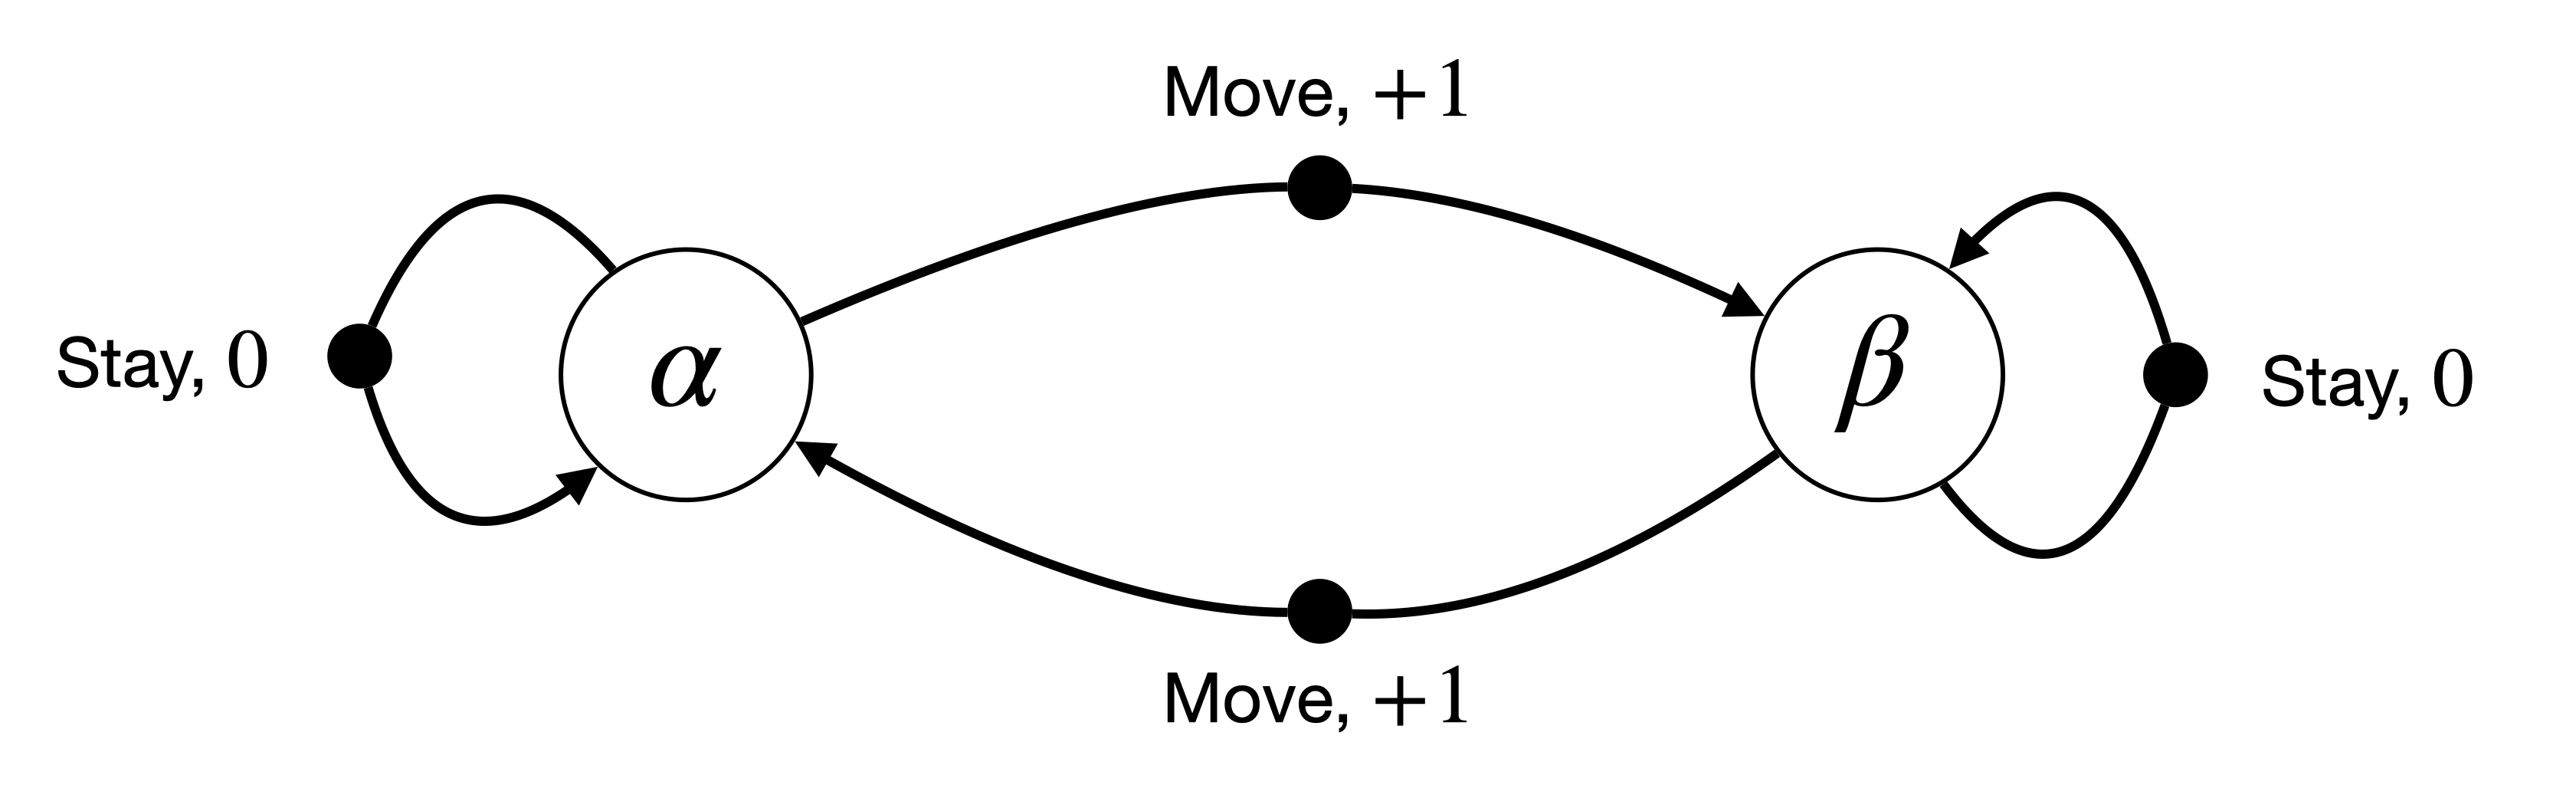
\includegraphics[width=0.9\linewidth]{images/MDP/robot-mdp-graph} 

}

\caption{A Simple Transition Graph.}\label{fig:mdp-robot-transition-graph}
\end{figure}

At time \(t=0\), if the robot starts at \(s_0 = \alpha\), first chooses action \(a_0 = \text{Move}\), and then chooses action \(a_1 = \text{Stay}\), the resulting trajectory is
\[
\tau = (\alpha, \text{Move}, +1, \beta, \text{Stay}, 0,  \beta).
\]
The return of this trajectory is:
\[
g_0 = +1 + 0 = +1.
\]

\textbf{Policy Evaluation}. Given a policy
\begin{equation}
\pi = (\pi_0, \pi_1), \quad \pi_0(a \mid s) = \begin{cases}
0.5 & a = \text{Move} \\
0.5 & a = \text{Stay}
\end{cases}, 
\quad 
\pi_1( a \mid s) = \begin{cases}
0.8 & a = \text{Move} \\
0.2 & a = \text{Stay}
\end{cases}.
\end{equation}
We can use the Bellman consistency equations to compute the state-value function. We first initialize:
\[
V^{\pi}_2 = \begin{bmatrix}
0 \\ 0
\end{bmatrix},
\]
where the first row contains the value at \(s = \alpha\) and the second row contains the value at \(s = \beta\).
We then perform the backward recursion for \(t=1\). For \(s = \alpha\), we have
\begin{equation}
V^{\pi}_1(\alpha) = \begin{bmatrix}
\pi_1(\text{Move} \mid \alpha) \\
\pi_1(\text{Stay} \mid \alpha)
\end{bmatrix}^{\top} \begin{bmatrix}
R(\alpha, \text{Move}) + V^{\pi}_2(\beta) \\
R(\alpha, \text{Stay}) + V^{\pi}_2(\alpha)
\end{bmatrix} = \begin{bmatrix}
0.8 \\ 0.2
\end{bmatrix}^{\top}
\begin{bmatrix}
1 \\ 0
\end{bmatrix} = 0.8 
\end{equation}
For \(s = \beta\), we have
\begin{equation}
V^{\pi}_1(\beta) = \begin{bmatrix}
\pi_1(\text{Move} \mid \beta) \\
\pi_1(\text{Stay} \mid \beta)
\end{bmatrix}^{\top} \begin{bmatrix}
R(\beta, \text{Move}) + V^{\pi}_2(\alpha) \\
R(\beta, \text{Stay}) + V^{\pi}_2(\beta)
\end{bmatrix} = \begin{bmatrix}
0.8 \\ 0.2
\end{bmatrix}^{\top}
\begin{bmatrix}
1 \\ 0
\end{bmatrix} = 0.8.
\end{equation}
Therefore, we have
\[
V^{\pi}_1 = \begin{bmatrix}
0.8 \\ 0.8
\end{bmatrix}.
\]
We then proceed to the backward recursion for \(t=0\):
\begin{align}
V_0^{\pi}(\alpha) & = \begin{bmatrix}
\pi_0(\text{Move} \mid \alpha) \\
\pi_0(\text{Stay} \mid \alpha)
\end{bmatrix}^{\top} \begin{bmatrix}
R(\alpha, \text{Move}) + V^{\pi}_1(\beta) \\
R(\alpha, \text{Stay}) + V^{\pi}_1(\alpha)
\end{bmatrix} = \begin{bmatrix}
0.5 \\ 0.5
\end{bmatrix}^{\top}
\begin{bmatrix}
1.8 \\ 0.8
\end{bmatrix} = 1.3. \\
V_0^{\pi}(\beta) & = \begin{bmatrix}
\pi_0(\text{Move} \mid \beta) \\
\pi_0(\text{Stay} \mid \beta)
\end{bmatrix}^{\top} \begin{bmatrix}
R(\beta, \text{Move}) + V^{\pi}_0(\alpha) \\
R(\beta, \text{Stay}) + V^{\pi}_0(\beta)
\end{bmatrix} = \begin{bmatrix}
0.5 \\ 0.5
\end{bmatrix}^{\top}
\begin{bmatrix}
1.8 \\ 0.8
\end{bmatrix} = 1.3.
\end{align}
Therefore, the state-value function at \(t=0\) is
\[
V^{\pi}_0 = \begin{bmatrix}
1.3 \\ 1.3
\end{bmatrix}.
\]
You are encouraged to carry out the similar calculations for the action-value function.

\begin{center}\rule{0.5\linewidth}{0.5pt}\end{center}

The toy example was small enough to carry out policy evaluation by hand; in realistic MDPs, we will need the help from computers.

Consider now an MDP whose transition graph is shown in Fig. \ref{fig:mdp-hangover-transition-graph}. This example is adapted from \href{https://github.com/upb-lea/reinforcement_learning_course_materials/blob/master/exercises/solutions/ex02/Ex2.ipynb}{here}.

\begin{figure}

{\centering 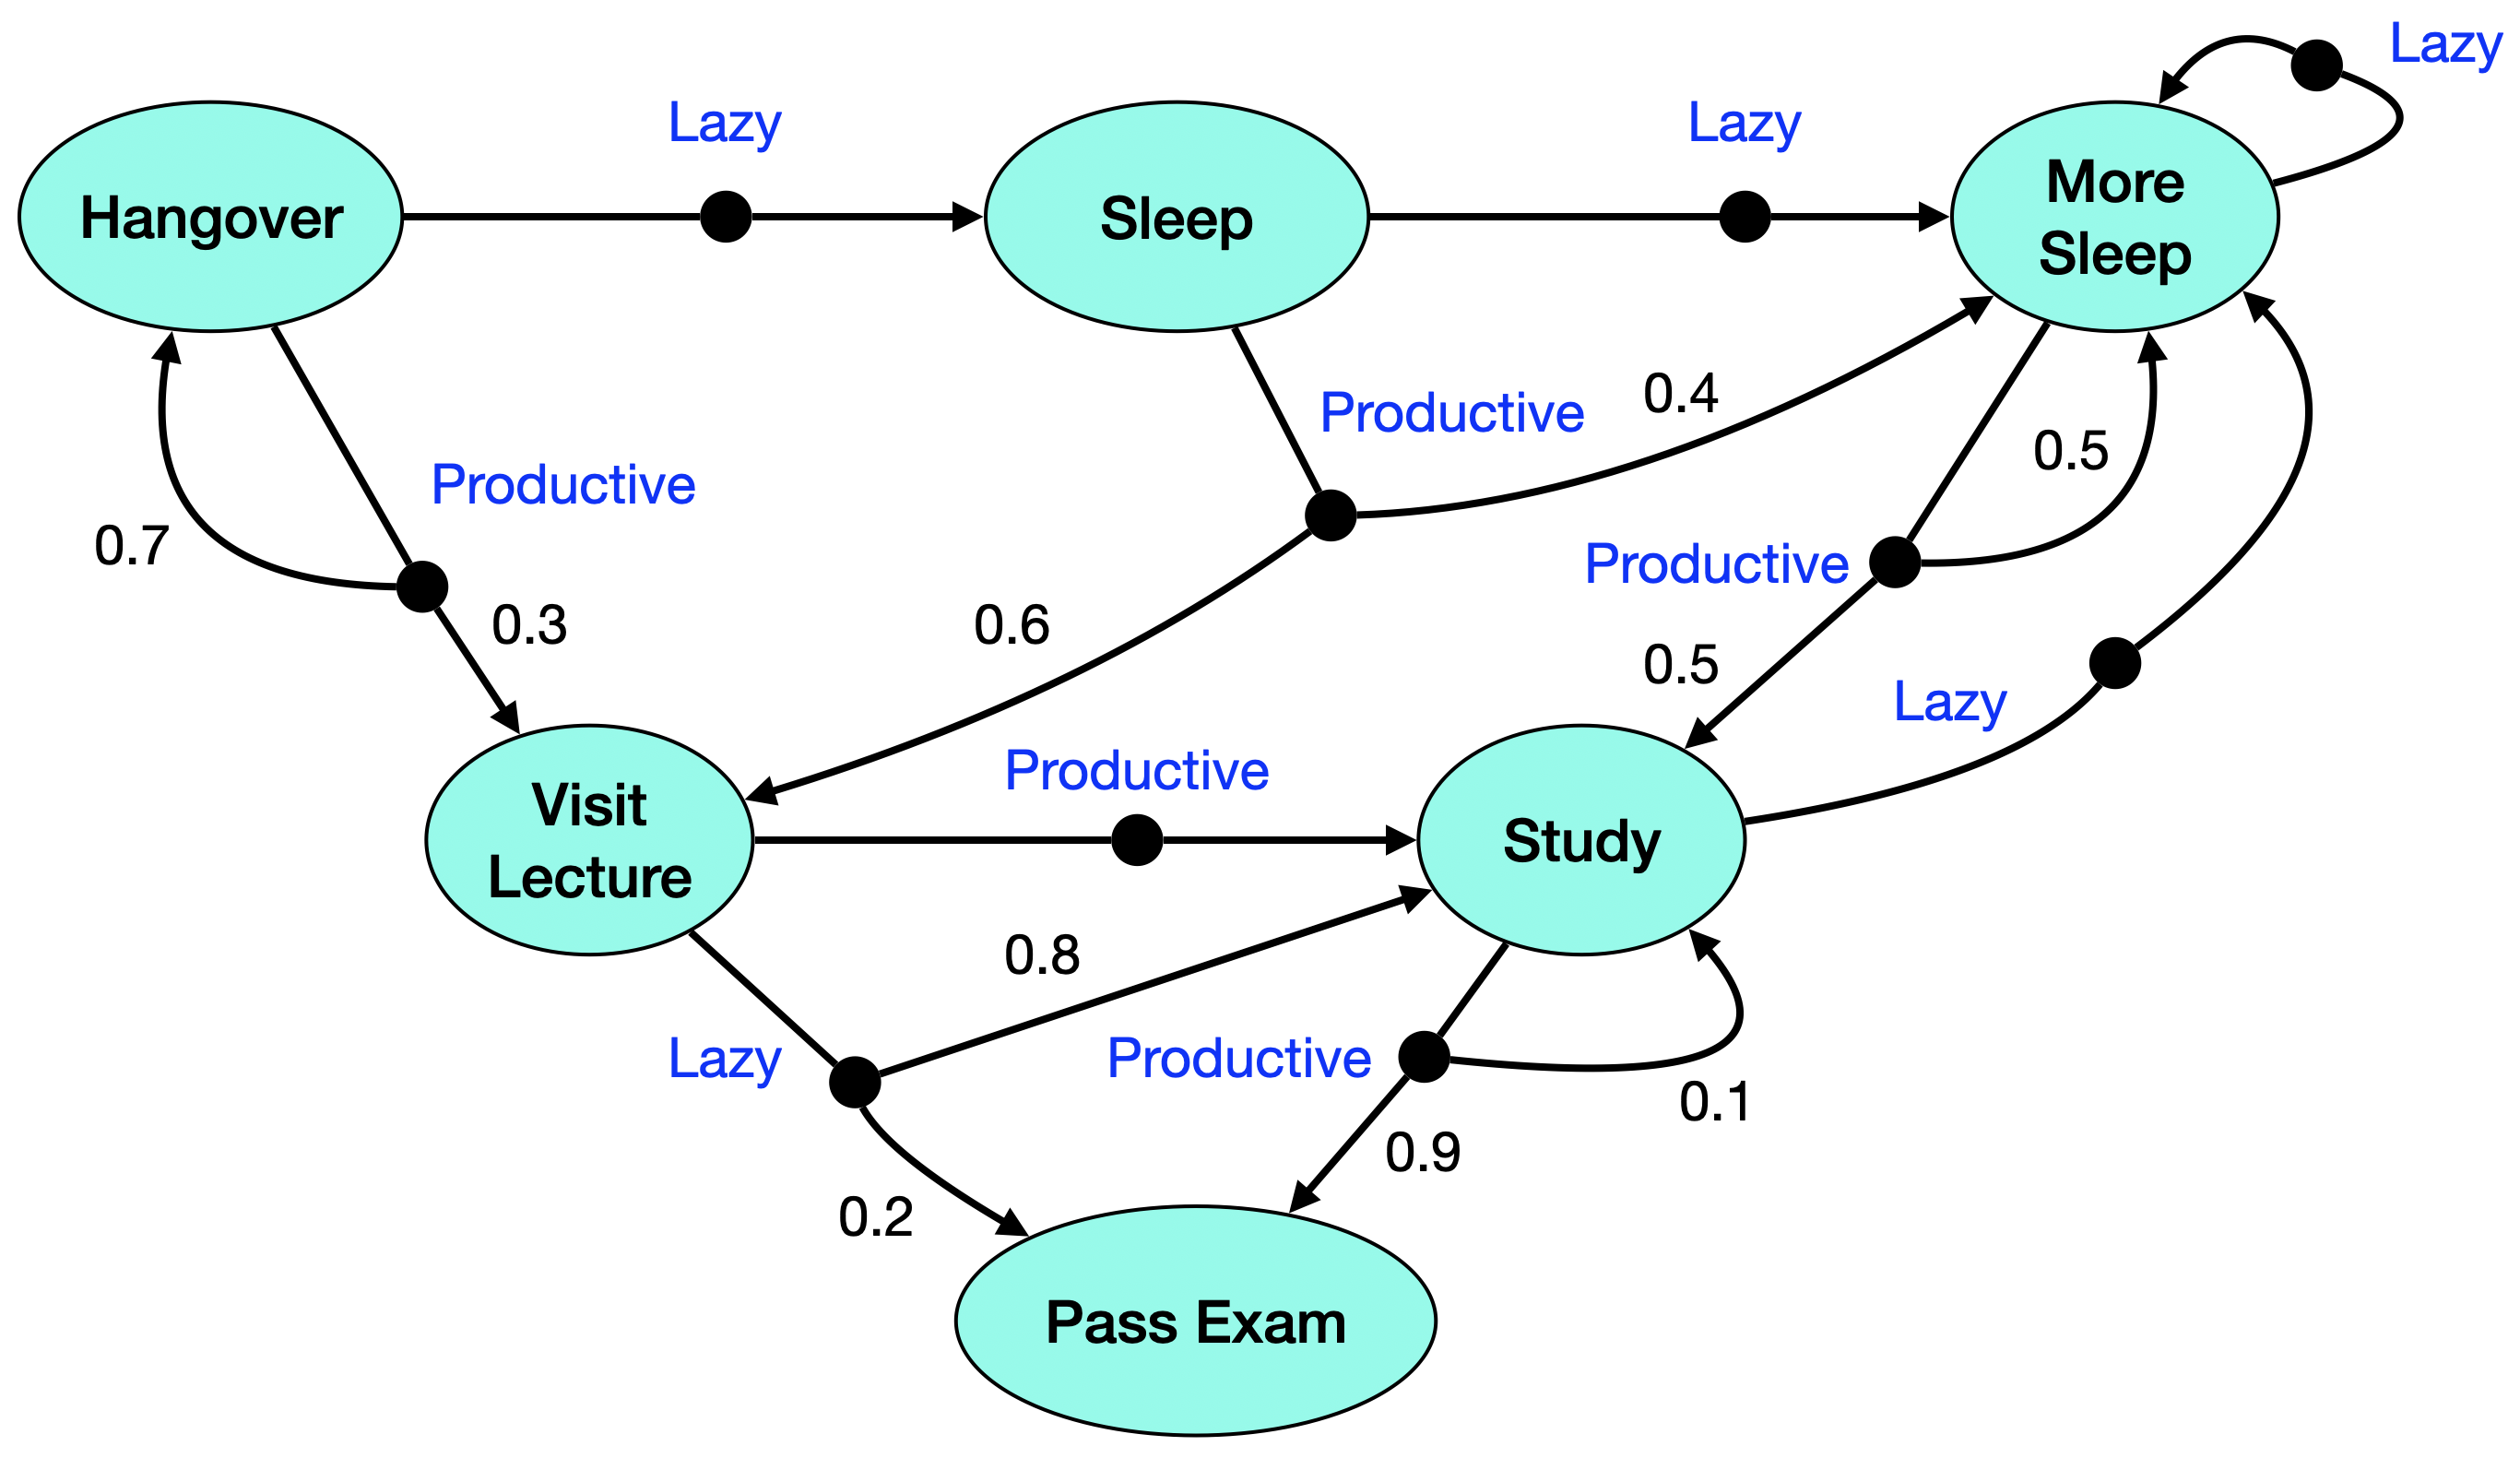
\includegraphics[width=0.9\linewidth]{images/MDP/hangover-graph} 

}

\caption{Hangover Transition Graph.}\label{fig:mdp-hangover-transition-graph}
\end{figure}

This MDP has six states:
\[
\mathcal{S} = \{\text{Hangover}, \text{Sleep}, \text{More Sleep}, \text{Visit Lecture}, \text{Study}, \text{Pass Exam} \},
\]
and two actions:
\[
\mathcal{A} = \{\text{Lazy}, \text{Productive} \}.
\]
The stochastic transition dynamics are labeled in the transition graph. For example, at state ``Hangover'', taking action ``Productive'' will lead to state ``Visit Lecture'' with probability \(0.3\) and state ``Hangover'' with probability \(0.7\).
The rewards of the MDP are defined as:
\[
R(s,a) = \begin{cases}
+1 & s = \text{Pass Exam} \\
-1 & \text{otherwise}.
\end{cases}.
\]

\textbf{Policy Evaluation}. Consider a time-invariant random policy
\[
\pi = \{\pi_0,\dots,\pi_{T-1} \}, \quad \pi_t(a \mid s) = \begin{cases}
\alpha & a = \text{Lazy} \\
1 - \alpha & a = \text{Productive}
\end{cases},
\]
that takes ``Lazy'' with probability \(\alpha\) and ``Productive'' with probability \(1-\alpha\).

The following Python code performs policy evaluation for this MDP, with \(T=10\) and \(\alpha = 0.4\).

\begin{Shaded}
\begin{Highlighting}[]
\CommentTok{\# Finite{-}horizon policy evaluation for the Hangover MDP}

\ImportTok{from}\NormalTok{ collections }\ImportTok{import}\NormalTok{ defaultdict}
\ImportTok{from}\NormalTok{ typing }\ImportTok{import}\NormalTok{ Dict, List, Tuple}

\NormalTok{State }\OperatorTok{=} \BuiltInTok{str}
\NormalTok{Action }\OperatorTok{=} \BuiltInTok{str}

\CommentTok{\# {-}{-}{-} MDP spec {-}{-}{-}{-}{-}{-}{-}{-}{-}{-}{-}{-}{-}{-}{-}{-}{-}{-}{-}{-}{-}{-}{-}{-}{-}{-}{-}{-}{-}{-}{-}{-}{-}{-}{-}{-}{-}{-}{-}{-}{-}{-}{-}{-}{-}{-}{-}{-}{-}{-}{-}{-}{-}{-}{-}{-}{-}{-}{-}{-}{-}{-}{-}}

\NormalTok{S: List[State] }\OperatorTok{=}\NormalTok{ [}
    \StringTok{"Hangover"}\NormalTok{, }\StringTok{"Sleep"}\NormalTok{, }\StringTok{"More Sleep"}\NormalTok{, }\StringTok{"Visit Lecture"}\NormalTok{, }\StringTok{"Study"}\NormalTok{, }\StringTok{"Pass Exam"}
\NormalTok{]}
\NormalTok{A: List[Action] }\OperatorTok{=}\NormalTok{ [}\StringTok{"Lazy"}\NormalTok{, }\StringTok{"Productive"}\NormalTok{]}

\CommentTok{\# P[s, a] {-}\textgreater{} list of (s\_next, prob)}
\NormalTok{P: Dict[Tuple[State, Action], List[Tuple[State, }\BuiltInTok{float}\NormalTok{]]] }\OperatorTok{=}\NormalTok{ \{}
    \CommentTok{\# Hangover}
\NormalTok{    (}\StringTok{"Hangover"}\NormalTok{, }\StringTok{"Lazy"}\NormalTok{):       [(}\StringTok{"Sleep"}\NormalTok{, }\FloatTok{1.0}\NormalTok{)],}
\NormalTok{    (}\StringTok{"Hangover"}\NormalTok{, }\StringTok{"Productive"}\NormalTok{): [(}\StringTok{"Visit Lecture"}\NormalTok{, }\FloatTok{0.3}\NormalTok{), (}\StringTok{"Hangover"}\NormalTok{, }\FloatTok{0.7}\NormalTok{)],}

    \CommentTok{\# Sleep}
\NormalTok{    (}\StringTok{"Sleep"}\NormalTok{, }\StringTok{"Lazy"}\NormalTok{):          [(}\StringTok{"More Sleep"}\NormalTok{, }\FloatTok{1.0}\NormalTok{)],}
\NormalTok{    (}\StringTok{"Sleep"}\NormalTok{, }\StringTok{"Productive"}\NormalTok{):    [(}\StringTok{"Visit Lecture"}\NormalTok{, }\FloatTok{0.6}\NormalTok{), (}\StringTok{"More Sleep"}\NormalTok{, }\FloatTok{0.4}\NormalTok{)],}

    \CommentTok{\# More Sleep}
\NormalTok{    (}\StringTok{"More Sleep"}\NormalTok{, }\StringTok{"Lazy"}\NormalTok{):       [(}\StringTok{"More Sleep"}\NormalTok{, }\FloatTok{1.0}\NormalTok{)],}
\NormalTok{    (}\StringTok{"More Sleep"}\NormalTok{, }\StringTok{"Productive"}\NormalTok{): [(}\StringTok{"Study"}\NormalTok{, }\FloatTok{0.5}\NormalTok{), (}\StringTok{"More Sleep"}\NormalTok{, }\FloatTok{0.5}\NormalTok{)],}

    \CommentTok{\# Visit Lecture}
\NormalTok{    (}\StringTok{"Visit Lecture"}\NormalTok{, }\StringTok{"Lazy"}\NormalTok{):       [(}\StringTok{"Study"}\NormalTok{, }\FloatTok{0.8}\NormalTok{), (}\StringTok{"Pass Exam"}\NormalTok{, }\FloatTok{0.2}\NormalTok{)],}
\NormalTok{    (}\StringTok{"Visit Lecture"}\NormalTok{, }\StringTok{"Productive"}\NormalTok{): [(}\StringTok{"Study"}\NormalTok{, }\FloatTok{1.0}\NormalTok{)],}

    \CommentTok{\# Study}
\NormalTok{    (}\StringTok{"Study"}\NormalTok{, }\StringTok{"Lazy"}\NormalTok{):         [(}\StringTok{"More Sleep"}\NormalTok{, }\FloatTok{1.0}\NormalTok{)],}
\NormalTok{    (}\StringTok{"Study"}\NormalTok{, }\StringTok{"Productive"}\NormalTok{):   [(}\StringTok{"Pass Exam"}\NormalTok{, }\FloatTok{0.9}\NormalTok{), (}\StringTok{"Study"}\NormalTok{, }\FloatTok{0.1}\NormalTok{)],}

    \CommentTok{\# Pass Exam (absorbing)}
\NormalTok{    (}\StringTok{"Pass Exam"}\NormalTok{, }\StringTok{"Lazy"}\NormalTok{):       [(}\StringTok{"Pass Exam"}\NormalTok{, }\FloatTok{1.0}\NormalTok{)],}
\NormalTok{    (}\StringTok{"Pass Exam"}\NormalTok{, }\StringTok{"Productive"}\NormalTok{): [(}\StringTok{"Pass Exam"}\NormalTok{, }\FloatTok{1.0}\NormalTok{)],}
\NormalTok{\}}

\KeywordTok{def}\NormalTok{ R(s: State, a: Action) }\OperatorTok{{-}\textgreater{}} \BuiltInTok{float}\NormalTok{:}
    \CommentTok{"""Reward: +1 in Pass Exam, {-}1 otherwise."""}
    \ControlFlowTok{return} \FloatTok{1.0} \ControlFlowTok{if}\NormalTok{ s }\OperatorTok{==} \StringTok{"Pass Exam"} \ControlFlowTok{else} \OperatorTok{{-}}\FloatTok{1.0}

\CommentTok{\# {-}{-}{-} Policy: time{-}invariant, state{-}independent {-}{-}{-}{-}{-}{-}{-}{-}{-}{-}{-}{-}{-}{-}{-}{-}{-}{-}{-}{-}{-}{-}{-}{-}{-}{-}{-}{-}{-}{-}}

\KeywordTok{def}\NormalTok{ pi(a: Action, s: State, alpha: }\BuiltInTok{float}\NormalTok{) }\OperatorTok{{-}\textgreater{}} \BuiltInTok{float}\NormalTok{:}
    \CommentTok{"""π(a|s): Lazy with prob α, Productive with prob 1{-}α."""}
    \ControlFlowTok{return}\NormalTok{ alpha }\ControlFlowTok{if}\NormalTok{ a }\OperatorTok{==} \StringTok{"Lazy"} \ControlFlowTok{else}\NormalTok{ (}\FloatTok{1.0} \OperatorTok{{-}}\NormalTok{ alpha)}

\CommentTok{\# {-}{-}{-} Policy evaluation {-}{-}{-}{-}{-}{-}{-}{-}{-}{-}{-}{-}{-}{-}{-}{-}{-}{-}{-}{-}{-}{-}{-}{-}{-}{-}{-}{-}{-}{-}{-}{-}{-}{-}{-}{-}{-}{-}{-}{-}{-}{-}{-}{-}{-}{-}{-}{-}{-}{-}{-}{-}{-}{-}{-}}

\KeywordTok{def}\NormalTok{ policy\_evaluation(T: }\BuiltInTok{int}\NormalTok{, alpha: }\BuiltInTok{float}\NormalTok{):}
    \CommentTok{"""}
\CommentTok{    Compute \{V\_t(s)\} and \{Q\_t(s,a)\} for t=0..T with terminal condition V\_T = Q\_T = 0.}
\CommentTok{    Returns:}
\CommentTok{        V: Dict[int, Dict[State, float]]}
\CommentTok{        Q: Dict[int, Dict[Tuple[State, Action], float]]}
\CommentTok{    """}
    \ControlFlowTok{assert}\NormalTok{ T }\OperatorTok{\textgreater{}=} \DecValTok{0}
    \CommentTok{\# sanity: probabilities sum to 1 for each (s,a)}
    \ControlFlowTok{for}\NormalTok{ key, rows }\KeywordTok{in}\NormalTok{ P.items():}
\NormalTok{        total }\OperatorTok{=} \BuiltInTok{sum}\NormalTok{(p }\ControlFlowTok{for}\NormalTok{ \_, p }\KeywordTok{in}\NormalTok{ rows)}
        \ControlFlowTok{if} \BuiltInTok{abs}\NormalTok{(total }\OperatorTok{{-}} \FloatTok{1.0}\NormalTok{) }\OperatorTok{\textgreater{}} \FloatTok{1e{-}9}\NormalTok{:}
            \ControlFlowTok{raise} \PreprocessorTok{ValueError}\NormalTok{(}\SpecialStringTok{f"Probabilities for }\SpecialCharTok{\{}\NormalTok{key}\SpecialCharTok{\}}\SpecialStringTok{ sum to }\SpecialCharTok{\{}\NormalTok{total}\SpecialCharTok{\}}\SpecialStringTok{, not 1."}\NormalTok{)}

\NormalTok{    V: Dict[}\BuiltInTok{int}\NormalTok{, Dict[State, }\BuiltInTok{float}\NormalTok{]] }\OperatorTok{=}\NormalTok{ defaultdict(}\BuiltInTok{dict}\NormalTok{)}
\NormalTok{    Q: Dict[}\BuiltInTok{int}\NormalTok{, Dict[Tuple[State, Action], }\BuiltInTok{float}\NormalTok{]] }\OperatorTok{=}\NormalTok{ defaultdict(}\BuiltInTok{dict}\NormalTok{)}

    \CommentTok{\# Terminal boundary}
    \ControlFlowTok{for}\NormalTok{ s }\KeywordTok{in}\NormalTok{ S:}
\NormalTok{        V[T][s] }\OperatorTok{=} \FloatTok{0.0}
        \ControlFlowTok{for}\NormalTok{ a }\KeywordTok{in}\NormalTok{ A:}
\NormalTok{            Q[T][(s, a)] }\OperatorTok{=} \FloatTok{0.0}

    \CommentTok{\# Backward recursion}
    \ControlFlowTok{for}\NormalTok{ t }\KeywordTok{in} \BuiltInTok{range}\NormalTok{(T }\OperatorTok{{-}} \DecValTok{1}\NormalTok{, }\OperatorTok{{-}}\DecValTok{1}\NormalTok{, }\OperatorTok{{-}}\DecValTok{1}\NormalTok{):}
        \ControlFlowTok{for}\NormalTok{ s }\KeywordTok{in}\NormalTok{ S:}
            \CommentTok{\# First compute Q\_t(s,a)}
            \ControlFlowTok{for}\NormalTok{ a }\KeywordTok{in}\NormalTok{ A:}
\NormalTok{                exp\_next }\OperatorTok{=} \BuiltInTok{sum}\NormalTok{(p }\OperatorTok{*}\NormalTok{ V[t }\OperatorTok{+} \DecValTok{1}\NormalTok{][s\_next] }\ControlFlowTok{for}\NormalTok{ s\_next, p }\KeywordTok{in}\NormalTok{ P[(s, a)])}
\NormalTok{                Q[t][(s, a)] }\OperatorTok{=}\NormalTok{ R(s, a) }\OperatorTok{+}\NormalTok{ exp\_next}
            \CommentTok{\# Then V\_t(s) = E\_\{a\textasciitilde{}π\}[Q\_t(s,a)]}
\NormalTok{            V[t][s] }\OperatorTok{=} \BuiltInTok{sum}\NormalTok{(pi(a, s, alpha) }\OperatorTok{*}\NormalTok{ Q[t][(s, a)] }\ControlFlowTok{for}\NormalTok{ a }\KeywordTok{in}\NormalTok{ A)}

    \ControlFlowTok{return}\NormalTok{ V, Q}

\CommentTok{\# {-}{-}{-} Example run {-}{-}{-}{-}{-}{-}{-}{-}{-}{-}{-}{-}{-}{-}{-}{-}{-}{-}{-}{-}{-}{-}{-}{-}{-}{-}{-}{-}{-}{-}{-}{-}{-}{-}{-}{-}{-}{-}{-}{-}{-}{-}{-}{-}{-}{-}{-}{-}{-}{-}{-}{-}{-}{-}{-}{-}{-}{-}{-}{-}{-}}

\ControlFlowTok{if} \VariableTok{\_\_name\_\_} \OperatorTok{==} \StringTok{"\_\_main\_\_"}\NormalTok{:}
\NormalTok{    T }\OperatorTok{=} \DecValTok{10}        \CommentTok{\# horizon}
\NormalTok{    alpha }\OperatorTok{=} \FloatTok{0.4}  \CommentTok{\# probability of choosing Lazy}
\NormalTok{    V, Q }\OperatorTok{=}\NormalTok{ policy\_evaluation(T}\OperatorTok{=}\NormalTok{T, alpha}\OperatorTok{=}\NormalTok{alpha)}

    \CommentTok{\# Print V\_0}
    \BuiltInTok{print}\NormalTok{(}\SpecialStringTok{f"V\_0(s) with T=}\SpecialCharTok{\{}\NormalTok{T}\SpecialCharTok{\}}\SpecialStringTok{, alpha=}\SpecialCharTok{\{}\NormalTok{alpha}\SpecialCharTok{\}}\SpecialStringTok{:"}\NormalTok{)}
    \ControlFlowTok{for}\NormalTok{ s }\KeywordTok{in}\NormalTok{ S:}
        \BuiltInTok{print}\NormalTok{(}\SpecialStringTok{f"  }\SpecialCharTok{\{}\NormalTok{s}\SpecialCharTok{:13s\}}\SpecialStringTok{: }\SpecialCharTok{\{}\NormalTok{V[}\DecValTok{0}\NormalTok{][s]}\SpecialCharTok{: .3f\}}\SpecialStringTok{"}\NormalTok{)}
\end{Highlighting}
\end{Shaded}

The code returns the following state values at \(t=0\):
\[
V^{\pi}_0 = \begin{bmatrix}
-3.582 \\ -2.306 \\ -2.180 \\ 1.757 \\ 2.939 \\ 10
\end{bmatrix},
\]
where the ordering of the states follows that defined in \(\mathcal{S}\).

You can find the code \href{https://github.com/ComputationalRobotics/2025-ES-AM-158-LECTURE-CODE/blob/main/hangover_policy_evaluation.py}{here}.
\end{example}

\section{Principle of Optimality}\label{optimality}

\section{Dynamic Programming}\label{dp}

\appendix


\chapter{Convex Analysis and Optimization}\label{appconvex}

\section{Theory}\label{appconvex-theory}

\subsection{Sets}\label{sets}

Convex set is one of the most important concepts in convex optimization. Checking convexity of sets is crucial to determining whether a problem is a convex problem. Here we will present some definitions of some set notations in convex optimization.

\begin{definition}[Affine set]
\protect\hypertarget{def:affineset}{}\label{def:affineset}A set \(C\subset \mathbb{R}^n\) is affine if the line through any two distinct points in \(C\) lies in \(C\), i.e., if for any \(x_1,x_2 \in C\) and any \(\theta \in \mathbb{R}\), we have \(\theta x_1 + (1-\theta)x_2 \in C\).
\end{definition}

\begin{definition}[Convex set]
\protect\hypertarget{def:convexset}{}\label{def:convexset}A set \(C\subset \mathbb{R}^n\) is convex if the line segment between any two distinct points in \(C\) lies in \(C\), i.e., if for any \(x_1,x_2 \in C\) and any \(\theta \in [0,1]\), we have \(\theta x_1 + (1-\theta)x_2 \in C\).
\end{definition}

\begin{definition}[Cone]
\protect\hypertarget{def:cone}{}\label{def:cone}A set \(C\subset \mathbb{R}^n\) is a cone if for any \(x\in C\) and any \(\theta\geq 0\), we have \(\theta x \in C\).
\end{definition}

\begin{definition}[Convex Cone]
\protect\hypertarget{def:convexcone}{}\label{def:convexcone}A set \(C\subset \mathbb{R}^n\) is a convex cone if \(C\) is convex and a cone.
\end{definition}

Below are some important examples of convex sets:

\begin{definition}[Hyperplane]
\protect\hypertarget{def:hyperplane}{}\label{def:hyperplane}A hyperplane is a set of the form \[\{x|a^Tx = b\}\]
\end{definition}

\begin{definition}[Halfspaces]
\protect\hypertarget{def:halfspaces}{}\label{def:halfspaces}A (closed) halfspace is a set of the form \[\{x|a^Tx \leq b\}\]
\end{definition}

\begin{definition}[Balls]
\protect\hypertarget{def:balls}{}\label{def:balls}A ball is a set of the form \[B(x,r) = \{y|\|y-x\|_2 \leq r\} = \{x+ru|\|u\|_2\leq 1\}\]
where \(r >0\).
\end{definition}

\begin{definition}[Ellipsoids]
\protect\hypertarget{def:ellipsoids}{}\label{def:ellipsoids}A ellipsoid is a set of the form \[\mathcal{E} = \{y|(y-x)^TP^{-1}(y-x)\leq 1\}\]
where \(P\) is symmetric and positive definite.
\end{definition}

\begin{definition}[Polyhedra]
\protect\hypertarget{def:polyhedra}{}\label{def:polyhedra}A polyhedra is defined as the solution set of a finite number of linear equalities
and inequalities: \[\mathcal{P} = \{x|a_j^Tx\leq b_j, j=1,...,m, c_k^Tx=d_k,k=1,...,p\}\]
\end{definition}

\begin{definition}[Norm ball]
\protect\hypertarget{def:normball}{}\label{def:normball}A norm ball \(B\) of radius \(r\) and a center \(x_c\) associated with the norm \(\|\cdot\|\) is defined as: \[B = \{x|\|x-x_c\|\leq r\}\]
\end{definition}

\begin{definition}[Norm cone]
\protect\hypertarget{def:normcone}{}\label{def:normcone}A norm cone \(C\) associated with the norm \(\|\cdot\|\) is defined as: \[C = \{(x,t)|\|x\|\leq t\}\subset \mathbb{R}^{n+1}\]
\end{definition}

Simplexes are important family of polyhedra. Suppose the \(k+1\) points \(v_0,...,v_k\in \mathbb{R}^n\) are affinely independent, which means \(v_1-v_0,...,v_k-v_0\) are linearly independent.

\begin{definition}[Simplex]
\protect\hypertarget{def:simplex}{}\label{def:simplex}A simplex \(C\) defined by points \(v_0,...,v_k\) is: \[C = \textbf{conv}\{v_0,...,v_k\} = \{\theta_0v_0 + ... \theta_kv_k|\theta \succeq 0, \textbf{1}^T\theta = 1\}\]
\end{definition}

Extremely important examples of convex sets are positive semidefinite cones:

\begin{definition}[Symmetric,positive semidefinite,positive definite matrices]
\protect\hypertarget{def:symmetricmatrices}{}\label{def:symmetricmatrices}\leavevmode

\begin{enumerate}
\def\labelenumi{\arabic{enumi}.}
\tightlist
\item
  Symmetric matrices: \(\textbf{S}^n = \{X\in\mathbb{R}^{n\times n}| X=X^T\}\)
\item
  Symmetric Positive Semidefinite matrices: \(\textbf{S}_+^n = \{X\in\textbf{S}^n| X\succeq0\}\)
\item
  Symmetric Positive definite matrices: \(\textbf{S}_{++}^n = \{X\in\textbf{S}^n| X\succ0\}\)
\end{enumerate}

\end{definition}

In most scenarios, the set we encounter is more complicated. In general it is extermely hard to determine whether a set in convex or not. But if the set is `generated' by some convex sets, we can easily determine its convexity. So let's focus on operations that preserve convexity:

\begin{proposition}
\protect\hypertarget{prp:operationpreserveconvexity}{}\label{prp:operationpreserveconvexity}

Assume \(S\) is convex, \(S_\alpha,\alpha\in\mathcal{A}\) is a family of convex sets. Following operations on convex sets will preserve convexity:

\begin{enumerate}
\def\labelenumi{\arabic{enumi}.}
\item
  Intersection: \(\bigcap_{\alpha\in\mathcal{A}}S_\alpha\) is convex.
\item
  Image under affine function: A function \(f:\mathbb{R}^n\to\mathbb{R}^m\) is affine if it has the form \(f(x) = Ax+b\). The image of \(S\) under affine function \(f\) is convex. I.e. \(f(S) = \{f(x)|x\in S\}\) is convex
\item
  Image under perspective function: We define the perspective function \(P:\mathbb{R}^{n+1}\), with domain \(\textbf{dom}P = \mathbb{R}^n\times \mathbb{R}_{++}\)(where \(\mathbb{R}_{++}=\{x\in \mathbb{R}|x>0\}\)) as \(P(z,t) = z/t\). The image of \(S\) under perspective function is convex.
\item
  Image under linear-fractional function: We define linear fractional function \(f:\mathbb{R}^n\to\mathbb{R}^m\) as:\(f(x) = (Ax+b)/(c^Tx+d)\) with \(\textbf{dom}f = \{x|c^Tx+d>0\|\). The image of \(S\) under linear fractional functions is convex.
\end{enumerate}

\end{proposition}

In some cases, the restrictions of \textbf{interior} is too strict. For example, imagine a plane in \(\mathbb{R}^3\). The interior of the plane is \(\emptyset\). But intuitively many property should be extended to this kind of situation. Because the points in the plane also lies `inside' the convex set. Thus, we will define \textbf{relative interior}. First we will define \textbf{affine hull}.

\begin{definition}[Affine hull]
\protect\hypertarget{def:affinehull}{}\label{def:affinehull}The affine hull of a set \(S\) is the smallest affine set that contains \(S\), which can be written as:
\[\text{aff}(S) = \{\sum_{i=1}^k\alpha_ix_i|k>0,x_i\in S,\alpha_i\in\mathbb{R},\sum_{i=1}^k\alpha_i=1\}\]
\end{definition}

\begin{definition}[Relative Interior]
\protect\hypertarget{def:relint}{}\label{def:relint}The relative interior of a set \(S\) (denoted \(\text{relint}(S)\)) is defined as its interior within the affine hull of \(S\). I.e.
\[\text{relint}(S):=\{x\in S: \text{there exists } \epsilon>0 \text{ such that }N_\epsilon \cap \text{aff}(S)\subset S\}\]
where \(N_\epsilon(x)\) is a ball of radius \(\epsilon\) centered on \(x\).
\end{definition}

\subsection{Convex function}\label{appconvex-theory-convexfunction}

In this section, let's define convex functions:

\begin{definition}[Convex function]
\protect\hypertarget{def:defcvxfunc}{}\label{def:defcvxfunc}A function \(f:\mathbb{R}^n\to\mathbb{R}\) is \textbf{convex} if \(\textbf{dom}\ f\) is convex and \(\forall x,y\in \textbf{dom}\ f\) and with \(\theta \in [0,1]\), we have:\[f(\theta x +(1-\theta)y)\leq \theta f(x) + (1-\theta)f(y)\]
The function is \textbf{strictly convex} if the inequality holds whenever \(x\neq y\) and \(\theta\in (0,1)\).
\end{definition}

If a function is differentiable, it will be easier for us to check its convexity:

\begin{proposition}[Conditions for Convex function]
\protect\hypertarget{prp:decidecvx}{}\label{prp:decidecvx}1.(First order condition) Suppose \(f\) is differentiable, then \(f\) is convex if and only if \(\textbf{dom} f\) is convex and \(\forall x,y\in \textbf{dom} f\), \[f(y)\geq f(x) +\nabla f(x)^T(y-x)\]
2.(Second order conditions) Suppose \(f\) is twice differentiable, then \(f\) is convex if and only if \(\textbf{dom} f\) is convex and \(\forall x\in \textbf{dom} f\), \[\nabla^2 f(x) \succeq \textbf{0}\]
\end{proposition}

For the same purpose, some operations that preserve the convexity of the convex functions are presented here:

\begin{proposition}[Operations that preserve convexity]
\protect\hypertarget{prp:preservecvx}{}\label{prp:preservecvx}Let \(f:\mathbb{R}^n\to\mathbb{R}\) be a convex function and \(g_1,...,g_n\) be convex functions. The following operations will preserve convexity of the function:

1.(Nonnegative weighted sum): A nonnegative weighted sum of convex functions: \[f = \omega_1f_1 + ... +\omega_mf_m\]

2.(Composition with an affine mapping) Suppose \(A\in \mathbb{R}^{n\times m}\) and \(b\in \mathbb{R}^n\), then \(g(x) = f(Ax+b)\) is convex.

3.(Pointwise maximum and supremum) \(g(x) = \max\{g_1(x),...,g_n(x)\}\) is convex. If \(h(x,y)\) is convex in \(x\) for each \(y\in\mathcal{A}\), then \(\sup_{y\in\mathcal{A}} h(x,y)\) is also convex in \(x\).

4.(Minimization) If \(h(x,y)\) is convex in \((x,y)\), and \(C\) is a convex nonempty set, then \(\inf_{x\in C} h(x,y)\) is convex in \(x\).

5.(Perspective of a function) The perspective of \(f\) is the function \(h:\mathbb{R}^{n+1}\to\mathbb{R}\) defined by: \(h(x,t) = tf(x/t)\) with domain \(\textbf{dom}\ h=\{(x,t)|x/t\in\textbf{dom} f,t>0\}\). And \(h\) is convex.
\end{proposition}

\subsection{Lagrange dual}\label{lagrange-dual}

We consider an optimization problem in the standard form (without assuming convexity of anything):
\begin{equation}
\begin{aligned}
p^* = \quad \min_{x} \quad & f_0(x)\\
\textrm{s.t.} \quad & f_i(x)\leq 0\quad i=1...,m\\
  & h_i(x) = 0\quad i=1,...,p   \\
\end{aligned}
\end{equation}

\begin{definition}[Lagrange dual function]
\protect\hypertarget{def:defdualfunc}{}\label{def:defdualfunc}The Lagrangian related to the problem above is defined as: \[L(x,\lambda,\nu)=f_0(x)+\sum_{i=1}^m\lambda_if_i(x)+\sum_{i=1}^p\nu_ih_i(x)\]
The Lagrange dual function is defined as: \[g(\lambda,\nu) = \inf_{x\in\mathcal{D}}L(x,\lambda,\nu)\]
\end{definition}

When the Lagrangian is unbounded below in \(x\), the dual function takes on the value \(-\infty\). Note that since the Lagrange dual function is a pointwise infimum of a family of affine functions of \((\lambda,\nu)\), so it's concave. The Lagrange dual function will give us lower bounds of the optimal value of the original problem: \[g(\lambda,\nu)\leq p^*\]. We can see that, the dual function can give a nontrivial lower bound only when \(\lambda\succeq 0\). Thus we can solve the following dual problem to get the best lower bound.

\begin{definition}[Lagrange dual problem]
\protect\hypertarget{def:defdualprob}{}\label{def:defdualprob}The lagrangian dual problem is defined as follows:
\begin{equation}
  \begin{aligned}
  d^* = \quad \max_{\lambda,\nu} \quad & g(\lambda,\nu)\\
  \textrm{s.t.} \quad & \lambda\succeq 0
  \end{aligned}
  \end{equation}
This is a convex optimization problem.
\end{definition}

We can easily see that \[d^*\leq p^*\] always hold. This property is called \textbf{weak duality}. If \[d^*=p^*\], it's called \textbf{strong duality}. Strong duality does not hold in general, but it usually holfs for convex problems. We can find conditions that guarantee strong duality in convex problems, which are called constrained qualifications. Slater's constraint qualification is a useful one.

\begin{theorem}[Slater's constraint qualification]
\protect\hypertarget{thm:slater}{}\label{thm:slater}Strong duality holds for a convex problem
\begin{equation}
  \begin{aligned}
  p^* = \quad \min_{x} \quad & f_0(x)\\
  \textrm{s.t.} \quad & f_i(x)\leq 0\quad i=1...,m\\
    & Ax=b   \\
  \end{aligned}
 \end{equation}
if it is strictly feasible, i.e.
\[\exists x\in\textbf{relint}\mathcal{D}:\quad f_i(x)<0,\quad i=1...m,\quad Ax=b\]
And the linear inequalities do not need to hold with strict inequality.
\end{theorem}

\subsection{KKT condition}\label{appconvex-theory-kkt}

Note that if strong duality holds, denote \(x^*\) to be primal optimal, and \((\lambda^*,\nu^*)\) to be dual optimal. Then:

\begin{equation}
  \begin{aligned}
  f_0(x^*) = g(\lambda^*,\nu^*) = & \inf_x(f_0(x)+\sum_{i=1}^m\lambda_i^*f_i(x)+\sum_{i=1}^p\nu_i^*h_i(x))\\
 \leq & f_0(x^*)+\sum_{i=1}^m\lambda_i^*f_i(x)+\sum_{i=1}^p\nu_i^*h_i(x)\\
 \leq & f_0(x^*)\\
  \end{aligned}
  \end{equation}

from this, combining \(\lambda^*\geq 0\) and \(f_i(x^*)\leq 0\), we can know that: \(\lambda_i^*f_i(x^*)=0\quad i=1\cdots m\). This means for \(\lambda_i^*\) and \(f_i(x^*)\), one of them must be zero, which is known as complementary slackness).

Thus we arrived at the following four conditions, which are called KKT conditions.

\begin{theorem}[Karush-Kuhn-Tucker(KKT) Conditions]
\protect\hypertarget{thm:KKT}{}\label{thm:KKT}

The following four conditions are called KKT conditions (for a problem with differentiable \(f_i,h_i\))

\begin{enumerate}
\def\labelenumi{\arabic{enumi}.}
\tightlist
\item
  Primal feasible: \(f_i(x) \leq 0,i,\cdots ,m,\ h_i(x) = 0,i=1,\cdots ,p\)
\item
  Dual feasible: \(\lambda\succeq0\)
\item
  Complementary slackness: \(\lambda_if_i(x)=0,i=1,\cdots,m\)
\item
  Gradient of Lagrangian with respect to \(x\) vanishes:\(\nabla f_0(x)+\sum_{i=1}^m\lambda_i\nabla f_i(x)+\sum_{i=1}^p\nu_i\nabla h_i(x) = 0\)
\end{enumerate}

\end{theorem}

From the discussion above, we know that if strong duality holds and \(x,\lambda,\nu\) are optimal, then they must satisfy the KKT conditions.

Also if \(x,\lambda,\nu\) satisfy KKT for a convex problem, then they are optimal. However, the converse is not generally true, since KKT condition implies strong duality. If Slater's condition is satisfied, then \(x\) is optimal if and only if there exist \(\lambda,\nu\) that satisfy KKT conditions. Sometimes, by solving the KKT system, we can derive the closed-form solution of a optimization directly. Also, sometimes we will use the residual of the KKT system as the termination condition.

In general, \(f_i,h_i\) may not be differentiable. There are also KKT conditions for them, which will include knowledge of subdifferential and will not be included here.

\section{Practice}\label{appconvex-practice}

\subsection{CVX Introduction}\label{cvx-introduction}

In the last section, we have learned basic concepts and theorems in convex optimization. In this section, on the other hand, we will introduce you how to model basic convex optimization problems with CVX, an easy-to-use MATLAB package. To install CVX, please refer to this \href{http://cvxr.com/cvx/doc/install.html}{page}. Note that every time you what to use the CVX package, you should add it to your MATLAB path. For example, if I install CVX package in the parent directory of my current directory with default directory name \texttt{cvx}, the following line should be added before your CVX codes:

\begin{Shaded}
\begin{Highlighting}[]
\VariableTok{addpath}\NormalTok{(}\VariableTok{genpath}\NormalTok{(}\StringTok{"../cvx/"}\NormalTok{))}\OperatorTok{;}
\end{Highlighting}
\end{Shaded}

With CVX, it is incredibly easy for us to define and solve a convex optimization problem. You just need to:

\begin{enumerate}
\def\labelenumi{\arabic{enumi}.}
\item
  define the variables.
\item
  define the objective function you want to minimize or maximize.
\item
  define the constraints.
\end{enumerate}

After running your codes, the optimal objective value is stored in the variable \texttt{cvx\_optval}, and the problem status is stored in the variable \texttt{cvx\_status} (when your problem is well-defined, this variable's value will be \texttt{Solved}). The optimal solutions will be stored in the variables you define.

Throughout this section, we will study five types of convex optimization problems: linear programming (LP), quadratic programming (QP), (convex) quadratically constrained quadratic programming (QCQP), second-order cone programming (SOCP), and semidefinite programming (SDP). Given two types of optimization problems \(A\) and \(B\), we say \(A < B\) if \(A\) can always be converted to \(B\) while the inverse is not true. Under this notation, we have
\begin{equation*}
   \text{LP} < \text{QP} < \text{QCQP} < \text{SOCP} < \text{SDP}
\end{equation*}

\subsection{Linear Programming (LP)}\label{linear-programming-lp}

\textbf{Definition.} An LP has the following form:
\begin{equation}
   \label{eq:app-lpdef}
   \begin{aligned}
      \min_{x \in \mathbb{R}^n} & \ c^T x \\
      \text{subject to } & A x \le b  
   \end{aligned}
\end{equation}
where \(x\) is the variable, \(A \in \mathbb{R}^{m\times n}, b \in \mathbb{R}^m\), and \(c \in \mathbb{R}^n\) are the parameters. Note that the constraint \(A x \le b\) already incorporates linear equality constraints. To see this, consider the constraint \(A' x = b'\), we can reformulate it as \(A x \le b\) by
\begin{equation*}
   \begin{bmatrix}
      A' \\ -A'
   \end{bmatrix} x \le \begin{bmatrix}
      b' \\ -b'
   \end{bmatrix}
\end{equation*}

\textbf{Example.} Consider the problem of minimizing a linear function \(c_1 x_1 + c_2 x_2\) over a rectangle \([-l_1, l_1] \times [-l_2, l_2]\). We can convert it to the standard LP form in \eqref{eq:app-lpdef} by simply setting \(c\) as \([c_1, \ c_2]^T\) and the linear inequality constraint as
\begin{equation*}
   \begin{bmatrix}
      1 & 0 \\ -1 & 0 \\ 0 & 1 \\ 0 & -1
   \end{bmatrix} \begin{bmatrix}
      x_1 \\ x_2
   \end{bmatrix} \le \begin{bmatrix}
      l_1 \\ l_1 \\ l_2 \\ l_2
   \end{bmatrix}
\end{equation*}

Corresponding CVX codes are shown below:

\begin{Shaded}
\begin{Highlighting}[]
\CommentTok{\%\% Define the LP example setting}
\VariableTok{c1} \OperatorTok{=} \FloatTok{2}\OperatorTok{;}
\VariableTok{c2} \OperatorTok{=} \OperatorTok{{-}}\FloatTok{5}\OperatorTok{;}
\VariableTok{l1} \OperatorTok{=} \FloatTok{3}\OperatorTok{;}
\VariableTok{l2} \OperatorTok{=} \FloatTok{7}\OperatorTok{;}
\CommentTok{\% parameters: c, A, b}
\VariableTok{c} \OperatorTok{=}\NormalTok{ [}\VariableTok{c1}\OperatorTok{;} \VariableTok{c2}\NormalTok{]}\OperatorTok{;}
\VariableTok{A} \OperatorTok{=}\NormalTok{ [}\FloatTok{1}\OperatorTok{,} \FloatTok{0}\OperatorTok{;} \OperatorTok{{-}}\FloatTok{1}\OperatorTok{,} \FloatTok{0}\OperatorTok{;} \FloatTok{0}\OperatorTok{,} \FloatTok{1}\OperatorTok{;} \FloatTok{0}\OperatorTok{,} \OperatorTok{{-}}\FloatTok{1}\NormalTok{]}\OperatorTok{;}
\VariableTok{b} \OperatorTok{=}\NormalTok{ [}\VariableTok{l1}\OperatorTok{;} \VariableTok{l1}\OperatorTok{;} \VariableTok{l2}\OperatorTok{;} \VariableTok{l2}\NormalTok{]}\OperatorTok{;}

\CommentTok{\%\% solve LP}
\VariableTok{cvx\_begin}
    \VariableTok{variable} \VariableTok{x}\NormalTok{(}\FloatTok{2}\NormalTok{)}\OperatorTok{;} \CommentTok{\% define variables [x1, x2]}
    \VariableTok{minimize}\NormalTok{(}\VariableTok{c}\OperatorTok{\textquotesingle{}} \OperatorTok{*} \VariableTok{x}\NormalTok{)}\OperatorTok{;} \CommentTok{\% define the objective}
    \VariableTok{subject} \VariableTok{to}
        \VariableTok{A} \OperatorTok{*} \VariableTok{x} \OperatorTok{\textless{}=} \VariableTok{b}\OperatorTok{;} \CommentTok{\% define the linear constraint}
\VariableTok{cvx\_end}
\end{Highlighting}
\end{Shaded}

\subsection{Quadratic Programming (QP)}\label{quadratic-programming-qp}

\textbf{Definition.} A QP has the following form:
\begin{align}
   \label{eq:app-qpdef}
   \min_{x \in \mathbb{R}^n} \ & \frac{1}{2} x^T P x + q^T x \\
   \text{subject to } & Gx \le h \\
   & Ax = b
\end{align}
where \(P \in \mathcal{S}_+^n, q\in \mathbb{R}^n, G \in \mathbb{R}^{m \times n}, h\in \mathbb{R}^m, A \in \mathbb{R}^{p \times n}, b \in \mathbb{R}^p\). Here \(\mathcal{S}_+^n\) denotes the set of positive semidefinite matrices of size \(n\times n\). Obviously, if we set \(P\) as zero, QP will degenerate to LP.

\textbf{Example.} Consider the problem of minimizing a quadratic function
\begin{equation*}
   f(x_1, x_2) = p_1 x_1^2 + 2p_2 x_1 x_2 + p_3 x_2^2 + q_1 x_1 + q_2 x_2
\end{equation*}
over a rectangle \([-l_1, l_1] \times [-l_2, l_2]\). Since \(P = 2 \begin{bmatrix}
   p_1 & p_2 \\ p_2 & p_3
\end{bmatrix} \succeq 0\), the following two conditions must hold:
\begin{equation*}
   \begin{cases}
      p_1 \ge 0 \\
      p_1 p_3 - 4 p_2^2 \ge 0
   \end{cases}
\end{equation*}
Same as in the LP example, \(G\) and \(h\) can be expressed as:
\begin{equation*}
   \begin{bmatrix}
      1 & 0 \\ -1 & 0 \\ 0 & 1 \\ 0 & -1
   \end{bmatrix} \begin{bmatrix}
      x_1 \\ x_2
   \end{bmatrix} \le \begin{bmatrix}
      l_1 \\ l_1 \\ l_2 \\ l_2
   \end{bmatrix}
\end{equation*}

Corresponding CVX codes are shown below:

\begin{Shaded}
\begin{Highlighting}[]
\CommentTok{\%\% Define the QP example setting}
\VariableTok{p1} \OperatorTok{=} \FloatTok{2}\OperatorTok{;}
\VariableTok{p2} \OperatorTok{=} \FloatTok{0.5}\OperatorTok{;}
\VariableTok{p3} \OperatorTok{=} \FloatTok{4}\OperatorTok{;}
\VariableTok{q1} \OperatorTok{=} \OperatorTok{{-}}\FloatTok{3}\OperatorTok{;}
\VariableTok{q2} \OperatorTok{=} \OperatorTok{{-}}\FloatTok{6.5}\OperatorTok{;}
\VariableTok{l1} \OperatorTok{=} \FloatTok{2}\OperatorTok{;}
\VariableTok{l2} \OperatorTok{=} \FloatTok{2.5}\OperatorTok{;}
\CommentTok{\% check if the generated P is positive semidefinite}
\VariableTok{tmp1} \OperatorTok{=}\NormalTok{ (}\VariableTok{p1} \OperatorTok{\textgreater{}=} \FloatTok{0}\NormalTok{)}\OperatorTok{;}
\VariableTok{tmp2} \OperatorTok{=}\NormalTok{ (}\VariableTok{p1}\OperatorTok{*}\VariableTok{p3} \OperatorTok{{-}} \FloatTok{4}\OperatorTok{*}\VariableTok{p2}\OperatorTok{\^{}}\FloatTok{2} \OperatorTok{\textgreater{}=} \FloatTok{0}\NormalTok{)}\OperatorTok{;}
\KeywordTok{if} \OperatorTok{\textasciitilde{}}\NormalTok{(}\VariableTok{tmp1} \OperatorTok{\&\&} \VariableTok{tmp2}\NormalTok{)}
    \VariableTok{error}\NormalTok{(}\StringTok{"P is not positve semidefinite!"}\NormalTok{)}\OperatorTok{;}
\KeywordTok{end}
\CommentTok{\% parameters: P, q, G, h}
\VariableTok{P} \OperatorTok{=} \FloatTok{2} \OperatorTok{*}\NormalTok{ [}\VariableTok{p1}\OperatorTok{,} \VariableTok{p2}\OperatorTok{;} \VariableTok{p2}\OperatorTok{,} \VariableTok{p3}\NormalTok{]}\OperatorTok{;}
\VariableTok{q} \OperatorTok{=}\NormalTok{ [}\VariableTok{q1}\OperatorTok{;} \VariableTok{q2}\NormalTok{]}\OperatorTok{;}
\VariableTok{G} \OperatorTok{=}\NormalTok{ [}\FloatTok{1}\OperatorTok{,} \FloatTok{0}\OperatorTok{;} \OperatorTok{{-}}\FloatTok{1}\OperatorTok{,} \FloatTok{0}\OperatorTok{;} \FloatTok{0}\OperatorTok{,} \FloatTok{1}\OperatorTok{;} \FloatTok{0}\OperatorTok{,} \OperatorTok{{-}}\FloatTok{1}\NormalTok{]}\OperatorTok{;}
\VariableTok{h} \OperatorTok{=}\NormalTok{ [}\VariableTok{l1}\OperatorTok{;} \VariableTok{l1}\OperatorTok{;} \VariableTok{l2}\OperatorTok{;} \VariableTok{l2}\NormalTok{]}\OperatorTok{;}

\CommentTok{\%\% Solve the QP problem}
\VariableTok{cvx\_begin}
    \VariableTok{variable} \VariableTok{x}\NormalTok{(}\FloatTok{2}\NormalTok{)}\OperatorTok{;} \CommentTok{\% define variables [x1; x2]}
    \CommentTok{\% define the objective, where quad\_form(x, P) = x\textquotesingle{}*P*x}
    \VariableTok{obj} \OperatorTok{=} \FloatTok{0.5} \OperatorTok{*} \VariableTok{quad\_form}\NormalTok{(}\VariableTok{x}\OperatorTok{,} \VariableTok{P}\NormalTok{) }\OperatorTok{+} \VariableTok{q}\OperatorTok{\textquotesingle{}} \OperatorTok{*} \VariableTok{x}\OperatorTok{;} 
    \VariableTok{minimize}\NormalTok{(}\VariableTok{obj}\NormalTok{)}\OperatorTok{;} 
    \VariableTok{subject} \VariableTok{to}
        \VariableTok{G} \OperatorTok{*} \VariableTok{x} \OperatorTok{\textless{}=} \VariableTok{h}\OperatorTok{;} \CommentTok{\% define the linear constraint}
\VariableTok{cvx\_end}
\end{Highlighting}
\end{Shaded}

\subsection{Quadratically Constrained Quadratic Programming (QCQP)}\label{quadratically-constrained-quadratic-programming-qcqp}

\textbf{Definition.} An (convex) QCQP has the following form:
\begin{align}
   \label{eq:app-qcqpdef}
   \min_{x \in \mathbb{R}^n} \ & \frac{1}{2} x^T P_0 x + q_0^T x \\
   \text{subject to } & \frac{1}{2} x^T P_i x + q_i^T x + r_i \le 0, \ i = 1 \dots m \\
   & Ax = b
\end{align}
where \(P_i \in \mathcal{S}_+^n, i = 0 \dots m\), \(q_i \in \mathbb{R}^n, i = 0 \dots m\), \(A \in \mathbb{R}^{p \times n}\), and \(b \in \mathbb{R}^p\). Note that in other literature, you may find a more general form of QCQP: they don't require \(P_i\)'s to be positive semidefinite. Yet in this case, the problem is non-convex and beyond our scope.

\textbf{Example.} We study the problem of getting the minimum distance between two ellipses. By convention, when the ellipses overlap, we set the minimum distance as \(0\). This problem can be exactly solved by (convex) QCQP.
Consider two ellipses of the following form:
\begin{equation*}
   \begin{cases}
      \frac{1}{2} \begin{bmatrix} y_1 \\ z_1 \end{bmatrix}^T K_1 \begin{bmatrix} y_1 \\ z_1 \end{bmatrix}
      + k_1^T \begin{bmatrix} y_1 \\ z_1 \end{bmatrix} + c_1 \le 0 \\ 
      \frac{1}{2} \begin{bmatrix} y_2 \\ z_2 \end{bmatrix}^T K_2 \begin{bmatrix} y_2 \\ z_2 \end{bmatrix}
      + k_2^T \begin{bmatrix} y_2 \\ z_2 \end{bmatrix} + c_2 \le 0 \\ 
   \end{cases}
\end{equation*}
where \([y_1, z_1]^T\) and \([y_2, z_2]^T\) are arbitrary points inside the two ellipses respectively. Also, two ensure the ellipses are well defined, we should enforce the following properties in \((K_i, k_i, c_i), i = 1, 2\): (1) \(K_i \succ 0\); (2) Let \(K_i =  L_i L_i^T\) be the Cholesky decomposition of \(K_i\). Then, ellipse \(i\) can be rewritten as:
\begin{equation*}
   \frac{1}{2} \parallel L_i^T \begin{bmatrix} y_i \\ z_i \end{bmatrix} - L_i^{-1} k_i \parallel^2 \le 
   \frac{1}{2} \parallel L_i^{-1} k_i \parallel^2 - c_i
\end{equation*}
Thus,
\begin{equation*}
   \frac{1}{2} \parallel L_i^{-1} k_i \parallel^2 - c_i > 0
\end{equation*}
With these two assumptions, we want to minimize:
\begin{equation*}
   \frac{1}{2} (y_1 - y_2)^2 + (z_1 - z_2)^2
\end{equation*}

Now, we construct \(P, q, r\)'s in QCQP with the above parameters. Define the variable \(x\) as \([y_1, z_1, y_2, z_2]\).

\begin{enumerate}
\def\labelenumi{(\arabic{enumi})}
\item
  \(P_0\) can be obtained from:
  \begin{equation*}
     \frac{1}{2} (y_1 - y_2)^2 + (z_1 - z_2)^2 = \frac{1}{2} \begin{bmatrix}
    y_1 \\ z_1 \\ y_2 \\ z_2
     \end{bmatrix}^T \begin{bmatrix}
    1 & 0 & -1 & 0 \\ 0 & 1 & 0 & -1 \\ -1 & 0 & 1 & 0 \\ 0 & -1 & 0 & 1
     \end{bmatrix} \begin{bmatrix}
    y_1 \\ z_1 \\ y_2 \\ z_2
     \end{bmatrix}
  \end{equation*}
\item
  \(P_1, q_1, r_1\) can be obtained from:
  \begin{equation*}
     \frac{1}{2} \begin{bmatrix} y_1 \\ z_1 \end{bmatrix}^T K_1 \begin{bmatrix} y_1 \\ z_1 \end{bmatrix}
    + k_1^T \begin{bmatrix} y_1 \\ z_1 \end{bmatrix} + c_1 
     = \frac{1}{2} x^T \begin{bmatrix}
    K_1 & O \\ O & O
     \end{bmatrix} + \begin{bmatrix}
    k_1 \\ O 
     \end{bmatrix}^T x + c_1 \le 0
  \end{equation*}
\item
  \(P_2, q_2, r_2\) can be obtained from:
  \begin{equation*}
     \frac{1}{2} \begin{bmatrix} y_2 \\ z_2 \end{bmatrix}^T K_2 \begin{bmatrix} y_2 \\ z_2 \end{bmatrix}
    + k_2^T \begin{bmatrix} y_2 \\ z_2 \end{bmatrix} + c_2
     = \frac{1}{2} x^T \begin{bmatrix}
    O & O \\ O & K_2
     \end{bmatrix} + \begin{bmatrix}
    O \\ k_2
     \end{bmatrix}^T x + c_2 \le 0
  \end{equation*}
\end{enumerate}

The corresponding codes are shown below. In this example, we test the minimum distance between a circle \(y_1^2 + z_1^2 \le 1\) and another circle \((y_2 - 2)^2 + (z_2 - 2)^2 \le 1\). You can check whether the result from QCQP aligns with your manual calculation.

\begin{Shaded}
\begin{Highlighting}[]
\CommentTok{\%\% Define the QCQP example setting}
\VariableTok{K1} \OperatorTok{=} \VariableTok{eye}\NormalTok{(}\FloatTok{2}\NormalTok{)}\OperatorTok{;}
\VariableTok{k1} \OperatorTok{=} \VariableTok{zeros}\NormalTok{(}\FloatTok{2}\OperatorTok{,} \FloatTok{1}\NormalTok{)}\OperatorTok{;}
\VariableTok{c1} \OperatorTok{=} \OperatorTok{{-}}\FloatTok{0.5}\OperatorTok{;}
\VariableTok{K2} \OperatorTok{=} \VariableTok{eye}\NormalTok{(}\FloatTok{2}\NormalTok{)}\OperatorTok{;}
\VariableTok{k2} \OperatorTok{=}\NormalTok{ [}\FloatTok{2}\OperatorTok{;} \FloatTok{2}\NormalTok{]}\OperatorTok{;}
\VariableTok{c2} \OperatorTok{=} \FloatTok{3.5}\OperatorTok{;}
\KeywordTok{if} \OperatorTok{\textasciitilde{}}\NormalTok{(}\VariableTok{if\_ellipse}\NormalTok{(}\VariableTok{K1}\OperatorTok{,} \VariableTok{k1}\OperatorTok{,} \VariableTok{c1}\NormalTok{) }\OperatorTok{\&\&} \VariableTok{if\_ellipse}\NormalTok{(}\VariableTok{K2}\OperatorTok{,} \VariableTok{k2}\OperatorTok{,} \VariableTok{c2}\NormalTok{))}
    \VariableTok{error}\NormalTok{(}\StringTok{"The example setting is not correct"}\NormalTok{)}\OperatorTok{;}
\KeywordTok{end}
\CommentTok{\% define parameters P0, P1, P2, q1, q2, r1, r2}
\VariableTok{P0} \OperatorTok{=}\NormalTok{ [}\FloatTok{1}\OperatorTok{,}\FloatTok{0}\OperatorTok{,{-}}\FloatTok{1}\OperatorTok{,}\FloatTok{0}\OperatorTok{;} \FloatTok{0}\OperatorTok{,}\FloatTok{1}\OperatorTok{,}\FloatTok{0}\OperatorTok{,{-}}\FloatTok{1}\OperatorTok{;} \OperatorTok{{-}}\FloatTok{1}\OperatorTok{,}\FloatTok{0}\OperatorTok{,}\FloatTok{1}\OperatorTok{,}\FloatTok{0}\OperatorTok{;} \FloatTok{0}\OperatorTok{,{-}}\FloatTok{1}\OperatorTok{,}\FloatTok{0}\OperatorTok{,}\FloatTok{1}\NormalTok{]}\OperatorTok{;}
\VariableTok{P1} \OperatorTok{=} \VariableTok{zeros}\NormalTok{(}\FloatTok{4}\OperatorTok{,} \FloatTok{4}\NormalTok{)}\OperatorTok{;}
\VariableTok{P1}\NormalTok{(}\FloatTok{1}\OperatorTok{:}\FloatTok{2}\OperatorTok{,} \FloatTok{1}\OperatorTok{:}\FloatTok{2}\NormalTok{) }\OperatorTok{=} \VariableTok{K1}\OperatorTok{;}
\VariableTok{P2} \OperatorTok{=} \VariableTok{zeros}\NormalTok{(}\FloatTok{4}\OperatorTok{,} \FloatTok{4}\NormalTok{)}\OperatorTok{;}
\VariableTok{P2}\NormalTok{(}\FloatTok{3}\OperatorTok{:}\FloatTok{4}\OperatorTok{,} \FloatTok{3}\OperatorTok{:}\FloatTok{4}\NormalTok{) }\OperatorTok{=} \VariableTok{K2}\OperatorTok{;}
\VariableTok{q1} \OperatorTok{=}\NormalTok{ [}\VariableTok{k1}\OperatorTok{;} \VariableTok{zeros}\NormalTok{(}\FloatTok{2}\OperatorTok{,} \FloatTok{1}\NormalTok{)]}\OperatorTok{;}
\VariableTok{q2} \OperatorTok{=}\NormalTok{ [}\VariableTok{zeros}\NormalTok{(}\FloatTok{2}\OperatorTok{,} \FloatTok{1}\NormalTok{)}\OperatorTok{;} \VariableTok{k2}\NormalTok{]}\OperatorTok{;}
\VariableTok{r1} \OperatorTok{=} \VariableTok{c1}\OperatorTok{;}
\VariableTok{r2} \OperatorTok{=} \VariableTok{c2}\OperatorTok{;}

\CommentTok{\%\% Solve the QCQP problem}
\VariableTok{cvx\_begin}
    \VariableTok{variable} \VariableTok{x}\NormalTok{(}\FloatTok{4}\NormalTok{)}\OperatorTok{;} \CommentTok{\% define variables [y1; z1; y2; z2]}
    \CommentTok{\% define the objective, where quad\_form(x, P) = x\textquotesingle{}*P*x}
    \VariableTok{obj} \OperatorTok{=} \FloatTok{0.5} \OperatorTok{*} \VariableTok{quad\_form}\NormalTok{(}\VariableTok{x}\OperatorTok{,} \VariableTok{P0}\NormalTok{)}\OperatorTok{;} 
    \VariableTok{minimize}\NormalTok{(}\VariableTok{obj}\NormalTok{)}\OperatorTok{;} 
    \VariableTok{subject} \VariableTok{to}
        \FloatTok{0.5} \OperatorTok{*} \VariableTok{quad\_form}\NormalTok{(}\VariableTok{x}\OperatorTok{,} \VariableTok{P1}\NormalTok{) }\OperatorTok{+} \VariableTok{q1}\OperatorTok{\textquotesingle{}} \OperatorTok{*} \VariableTok{x} \OperatorTok{+} \VariableTok{r1} \OperatorTok{\textless{}=} \FloatTok{0}\OperatorTok{;}
        \FloatTok{0.5} \OperatorTok{*} \VariableTok{quad\_form}\NormalTok{(}\VariableTok{x}\OperatorTok{,} \VariableTok{P2}\NormalTok{) }\OperatorTok{+} \VariableTok{q2}\OperatorTok{\textquotesingle{}} \OperatorTok{*} \VariableTok{x} \OperatorTok{+} \VariableTok{r2} \OperatorTok{\textless{}=} \FloatTok{0}\OperatorTok{;}
\VariableTok{cvx\_end}

\CommentTok{\%\% detect whether (K, k, c) generates a ellipse}
\KeywordTok{function} \VariableTok{flag} \OperatorTok{=} \VariableTok{if\_ellipse}\NormalTok{(}\VariableTok{K}\OperatorTok{,} \VariableTok{k}\OperatorTok{,} \VariableTok{c}\NormalTok{)}
    \VariableTok{L} \OperatorTok{=} \VariableTok{chol}\NormalTok{(}\VariableTok{K}\NormalTok{)}\OperatorTok{;}
    \VariableTok{radius\_square} \OperatorTok{=} \FloatTok{0.5} \OperatorTok{*} \VariableTok{norm}\NormalTok{(}\VariableTok{L} \OperatorTok{\textbackslash{}} \VariableTok{k}\NormalTok{)}\OperatorTok{\^{}}\FloatTok{2} \OperatorTok{{-}} \VariableTok{c}\OperatorTok{;} \CommentTok{\% L \textbackslash{} k = inv(L) * k}
    \VariableTok{flag} \OperatorTok{=}\NormalTok{ (}\VariableTok{radius\_square} \OperatorTok{\textgreater{}} \FloatTok{0}\NormalTok{)}\OperatorTok{;}
\KeywordTok{end}
\end{Highlighting}
\end{Shaded}

\subsection{Second-Order Cone Programming (SOCP)}\label{second-order-cone-programming-socp}

\textbf{Definition.} An SOCP has the following form:
\begin{align}
   \label{eq:app-socpdef}
   \min_{x \in \mathbb{R}^n} \ & f^T x \\
   \text{subject to } & || A_i x + b_i ||_2 \le c_i^T x + d_i, \ i = 1 \dots m \\
   & Fx = g
\end{align}
where \(f \in \mathbb{R}^n, A_i \in \mathbb{R}^{n_i \times n}, b_i \in \mathbb{R}^{n_i}, c_i \in \mathbb{R}^n, d_i \in \mathbb{R}, F \in \mathbb{R}^{p \times n}\), and \(g \in \mathbb{R}^p\).

\textbf{Example.} We consider the problem of stochastic linear programming:
\begin{align}
   \min_x \ & c^T x \\
   \text{subject to } & \mathbb{P}(a_i^T x \le b_i) \ge p, \ i = 1 \dots m \\
   & a_i \sim \mathcal{N}(\bar{a}_i, \Sigma_i), \ i = 1 \dots m
\end{align}
Here \(p\) should be more than \(0.5\). We show that this problem can be converted to a SOCP:

Since \(a_i \sim \mathcal{N}(\bar{a}_i, \Sigma_i)\), then \((a_i^T x - b_i) \sim \mathcal{N}(\bar{a}_i^T x - b_i, x^T \Sigma_i x)\). Standardize it:
\begin{equation*}
   t := ||\Sigma_i^{\frac{1}{2}} x||_2^{-1} \left\{ (a_i^T x - b_i) - (\bar{a}_i^T x - b_i) \right\} \sim \mathcal{N}(0, 1)
\end{equation*}
Then,
\begin{align}
   \mathbb{P}(a_i^T x \le b_i) & = \mathbb{P}(a_i^T x - b_i \le 0) \\
   & = \mathbb{P}(t \le -||\Sigma_i^{\frac{1}{2}} x||_2^{-1}(\bar{a}_i^T x - b_i)) \\
   & = \Phi(-||\Sigma_i^{\frac{1}{2}} x||_2^{-1}(\bar{a}_i^T x - b_i))
\end{align}
Here \(\Phi(\cdot)\) is the cumulative distribution function of the standard normal distribution:
\begin{equation*}
   \Phi(\xi) = \int_{-\infty}^{\xi} e^{-\frac{1}{2} t^2} \ dt
\end{equation*}
Thus,
\begin{align}
   & \mathbb{P}(a_i^T x \le b_i) \ge p \\
   \Longleftrightarrow & \Phi(-||\Sigma_i^{\frac{1}{2}} x||_2^{-1}(\bar{a}_i^T x - b_i)) \ge p \\
   \Longleftrightarrow & -||\Sigma_i^{\frac{1}{2}} x||_2^{-1}(\bar{a}_i^T x - b_i) \ge \Phi^{-1}(p) \\
   \Longleftrightarrow & \Phi^{-1}(p) ||\Sigma_i^{\frac{1}{2}} x||_2 \le b_i - \bar{a}_i^T x
\end{align}
which is exactly the same as inequality constraints in SOCP formulation. (You can see why we enforce \(p > 0.5\) here: otherwise \(\Phi^{-1}(p)\) will be negative and the constraint with not be an second-order cone.)

In the following code example, we set up four inequality constraints and let \(\bar{a}_i^T x \le b_i, \ i = 1 \dots 4\) form an square located at the origin of size \(2\). Then, for convenience, we set \(\Sigma_i \equiv \sigma^2 I\).

\begin{Shaded}
\begin{Highlighting}[]
\CommentTok{\%\% Define the SOCP example setting}
\VariableTok{bar\_a1} \OperatorTok{=}\NormalTok{ [}\FloatTok{1}\OperatorTok{;} \FloatTok{0}\NormalTok{]}\OperatorTok{;}
\VariableTok{b1} \OperatorTok{=} \FloatTok{1}\OperatorTok{;}
\VariableTok{bar\_a2} \OperatorTok{=}\NormalTok{ [}\FloatTok{0}\OperatorTok{;} \FloatTok{1}\NormalTok{]}\OperatorTok{;}
\VariableTok{b2} \OperatorTok{=} \FloatTok{1}\OperatorTok{;}
\VariableTok{bar\_a3} \OperatorTok{=}\NormalTok{ [}\OperatorTok{{-}}\FloatTok{1}\OperatorTok{;} \FloatTok{0}\NormalTok{]}\OperatorTok{;}
\VariableTok{b3} \OperatorTok{=} \FloatTok{1}\OperatorTok{;}
\VariableTok{bar\_a4} \OperatorTok{=}\NormalTok{ [}\FloatTok{0}\OperatorTok{;} \OperatorTok{{-}}\FloatTok{1}\NormalTok{]}\OperatorTok{;}
\VariableTok{b4} \OperatorTok{=} \FloatTok{1}\OperatorTok{;}
\VariableTok{sigma} \OperatorTok{=} \FloatTok{0.1}\OperatorTok{;} 
\VariableTok{c} \OperatorTok{=}\NormalTok{ [}\FloatTok{2}\OperatorTok{;} \FloatTok{3}\NormalTok{]}\OperatorTok{;}
\VariableTok{p} \OperatorTok{=} \FloatTok{0.9}\OperatorTok{;} \CommentTok{\% p should be more than 0.5}
\VariableTok{Phi\_inv} \OperatorTok{=} \VariableTok{norminv}\NormalTok{(}\VariableTok{p}\NormalTok{)}\OperatorTok{;} \CommentTok{\% get Phi\^{}\{{-}1\}(p)}

\CommentTok{\%\% Solve the SOCP problem}
\VariableTok{cvx\_begin}
    \VariableTok{variable} \VariableTok{x}\NormalTok{(}\FloatTok{2}\NormalTok{)}\OperatorTok{;} \CommentTok{\% define variables [x1; x2]}
    \VariableTok{minimize}\NormalTok{(}\VariableTok{c}\OperatorTok{\textquotesingle{}} \OperatorTok{*} \VariableTok{x}\NormalTok{)}\OperatorTok{;} 
    \VariableTok{subject} \VariableTok{to}
        \VariableTok{sigma}\OperatorTok{*}\VariableTok{Phi\_inv} \OperatorTok{*} \VariableTok{norm}\NormalTok{(}\VariableTok{x}\NormalTok{) }\OperatorTok{\textless{}=} \VariableTok{b1} \OperatorTok{{-}} \VariableTok{bar\_a1}\OperatorTok{\textquotesingle{}} \OperatorTok{*} \VariableTok{x}\OperatorTok{;}
        \VariableTok{sigma}\OperatorTok{*}\VariableTok{Phi\_inv} \OperatorTok{*} \VariableTok{norm}\NormalTok{(}\VariableTok{x}\NormalTok{) }\OperatorTok{\textless{}=} \VariableTok{b2} \OperatorTok{{-}} \VariableTok{bar\_a2}\OperatorTok{\textquotesingle{}} \OperatorTok{*} \VariableTok{x}\OperatorTok{;}
        \VariableTok{sigma}\OperatorTok{*}\VariableTok{Phi\_inv} \OperatorTok{*} \VariableTok{norm}\NormalTok{(}\VariableTok{x}\NormalTok{) }\OperatorTok{\textless{}=} \VariableTok{b3} \OperatorTok{{-}} \VariableTok{bar\_a3}\OperatorTok{\textquotesingle{}} \OperatorTok{*} \VariableTok{x}\OperatorTok{;}
        \VariableTok{sigma}\OperatorTok{*}\VariableTok{Phi\_inv} \OperatorTok{*} \VariableTok{norm}\NormalTok{(}\VariableTok{x}\NormalTok{) }\OperatorTok{\textless{}=} \VariableTok{b4} \OperatorTok{{-}} \VariableTok{bar\_a4}\OperatorTok{\textquotesingle{}} \OperatorTok{*} \VariableTok{x}\OperatorTok{;}
\VariableTok{cvx\_end}
\end{Highlighting}
\end{Shaded}

\subsection{Semidefinite Programming (SDP)}\label{semidefinite-programming-sdp}

\textbf{Definition.} An SDP has the following form:
\begin{align}
   \label{eq:app-sdpdef}
   \min_{X_i, x_i} \ & \sum_{i=1}^{n_s} C_i \cdot X_i + \sum_{i=1}^{n_u} c_i \cdot x_i \\
   \text{subject to } & \sum_{i=1}^{n_s} A_{i,j} \cdot X_i + \sum_{i=1}^{n_u} a_{i,j} \cdot x_i = b_j, \quad j = 1 \dots m \\
   & X_i \in \mathcal{S}_+^{D_i}, \quad i = 1 \dots n_s \\
   & x_i \in \mathbb{R}^{d_i}, \quad i = 1 \dots n_u  
\end{align}
where \(C_i, A_{i, j} \in \mathbb{R}^{D_i \times D_i}\), \(c_i, a_{i, j} \in \mathbb{R}^{d_i}\), and \(\cdot\) means element-wise product. For two square matrices \(A, B\), the dot product \(A \cdot B\) is equal to \(\text{tr}(A B)\); for two vectors \(a, b\), the dot product \(a \cdot b\) is the same as inner product \(a^T b\).

Note that actually there are many ``standard'' forms of SDP. For example, in the convex optimization theory part, you may find an SDP that looks like:
\begin{align}
   \min_X \ & C \cdot X \\
   \text{subject to } & A \cdot X = b \\
   & X \succeq 0
\end{align}
It is convenient for us to analyze the theoretical properties of SDP with this form. Also, in SDP solvers' User Guide, you may see more complex SDP forms which involve more general convex cones. For example, see \href{https://docs.mosek.com/10.0/toolbox/tutorial-sdo-shared.html\#doc-tutorial-sdo}{MOSEK's MATLAB API docs}. Here we turn to use the form of \eqref{eq:app-sdpdef} for two reasons: (1) it is general enough: our SDP example below can be converted to this form (also, SDPs from sum-of-squares programming in this book are exactly of the form \eqref{eq:app-sdpdef}); (2) it is more readable than more complex forms.

\textbf{Example.} We consider the problem of finding the minimum eigenvalue for a positive semidefinite matrix \(S\). We will show that this problem can be converted to \eqref{eq:app-sdpdef}. Since \(S\) is positive semidefinite, the finding procedure can be cast as
\begin{align}
    \max_\lambda & \ \lambda \\
    \text{subject to } & S - \lambda I \succeq 0
\end{align}
Now define an auxiliary matrix \(X := S - \lambda I\). We have
\begin{align}
    \min_{\lambda, X} & \ -\lambda \\
   \text{subject to } &  X + \lambda I = S \\
   & X \succeq 0
\end{align}
It is obvious that the linear matrix equality constraint \(X + \lambda I = S\) can be divided into several linear scalar equality constraints in \eqref{eq:app-sdpdef}. For example, we consider \(S \in \mathbb{S}_+^3\). Thereby \(X + \lambda I = S\) will lead to \(6\) linear equality constraints (We don't consider \(X\) is a symmetric matrix here, since most solvers will implicitly consider this. Thus, only the upper-triangular part of \(X\) and \(S\) are actually used in the equality construction.):
\begin{align}
   &  \begin{bmatrix}
      1 & 0 & 0 \\ 0 & 0 & 0 \\ 0 & 0 & 0
   \end{bmatrix} \cdot X  + \lambda = S[0, 0],  
    \begin{bmatrix}
      0 & 1 & 0 \\ 0 & 0 & 0 \\ 0 & 0 & 0
   \end{bmatrix} \cdot X  = S[0, 1],
    \begin{bmatrix}
      0 & 0 & 1 \\ 0 & 0 & 0 \\ 0 & 0 & 0
   \end{bmatrix} \cdot X  = S[0, 2] \\
   &  \begin{bmatrix}
      0 & 0 & 0 \\ 0 & 1 & 0 \\ 0 & 0 & 0
   \end{bmatrix} \cdot X  + \lambda = S[1, 1],
    \begin{bmatrix}
      0 & 0 & 0 \\ 0 & 0 & 1 \\ 0 & 0 & 0
   \end{bmatrix} \cdot X  = S[1, 2], 
    \begin{bmatrix}
      0 & 0 & 0 \\ 0 & 0 & 0 \\ 0 & 0 & 1
   \end{bmatrix} \cdot X  + \lambda = S[2, 2] 
\end{align}
Seems tedious? Fortunately, CVX provides a high-level API to handle these linear equality constraints: you just need to write down

\begin{Shaded}
\begin{Highlighting}[]
\VariableTok{X} \OperatorTok{+} \VariableTok{lam} \OperatorTok{*} \VariableTok{eye}\NormalTok{(}\FloatTok{3}\NormalTok{) }\OperatorTok{==} \VariableTok{S}\OperatorTok{;} \CommentTok{\% linear equality constraints: X + lam *I = S}
\end{Highlighting}
\end{Shaded}

CVX will autometically convert this high-level constraint to \eqref{eq:app-sdpdef} and pass them to the underlying solver.

To generate a ramdom \(S \in \mathcal{S}_+^3\), you just need to assign three nonnegative eigenvalues to the program. After that, an random \(S\) will be generated by \(S = Q \ \text{diag}(\lambda_1, \lambda_2, \lambda_3) \ Q^T\), where \(Q\) is random orthonormal matrix.

\begin{Shaded}
\begin{Highlighting}[]
\CommentTok{\%\% Define the SDP example setting}
\VariableTok{lam\_list} \OperatorTok{=}\NormalTok{ [}\FloatTok{0.7}\OperatorTok{;} \FloatTok{2.4}\OperatorTok{;} \FloatTok{3.7}\NormalTok{]}\OperatorTok{;}
\VariableTok{S} \OperatorTok{=} \VariableTok{generate\_random\_PD\_matrix}\NormalTok{(}\VariableTok{lam\_list}\NormalTok{)}\OperatorTok{;} \CommentTok{\% get a PD matrix S}

\CommentTok{\%\% Solve the SDP problem}
\VariableTok{cvx\_begin}
    \VariableTok{variable} \VariableTok{X}\NormalTok{(}\FloatTok{3}\OperatorTok{,} \FloatTok{3}\NormalTok{) }\VariableTok{symmetric}\OperatorTok{;}
    \VariableTok{variable} \VariableTok{lam}\OperatorTok{;} 
    \VariableTok{maximize}\NormalTok{(}\VariableTok{lam}\NormalTok{)}\OperatorTok{;} 
    \VariableTok{subject} \VariableTok{to}
        \CommentTok{\% here "==" should be read as "is in"}
        \VariableTok{X} \OperatorTok{==} \VariableTok{semidefinite}\NormalTok{(}\FloatTok{3}\NormalTok{)}\OperatorTok{;} 
        \VariableTok{X} \OperatorTok{+} \VariableTok{lam} \OperatorTok{*} \VariableTok{eye}\NormalTok{(}\FloatTok{3}\NormalTok{) }\OperatorTok{==} \VariableTok{S}\OperatorTok{;}
\VariableTok{cvx\_end}

\CommentTok{\% this function help to generate PD matrix of size 3*3 }
\CommentTok{\% if you provide the eigenvalues [lam\_1, lam\_2, lam\_3]}
\KeywordTok{function} \VariableTok{S} \OperatorTok{=} \VariableTok{generate\_random\_PD\_matrix}\NormalTok{(}\VariableTok{lam\_list}\NormalTok{)}
    \KeywordTok{if} \OperatorTok{\textasciitilde{}}\VariableTok{all}\NormalTok{(}\VariableTok{lam\_list} \OperatorTok{\textgreater{}=} \FloatTok{0}\NormalTok{) }\CommentTok{\% all eigenvalues \textgreater{}= 0}
        \VariableTok{error}\NormalTok{(}\StringTok{"All eigenvalues must be nonnegative."}\NormalTok{)}\OperatorTok{;}
    \KeywordTok{end}
    \VariableTok{D} \OperatorTok{=} \VariableTok{diag}\NormalTok{(}\VariableTok{lam\_list}\NormalTok{)}\OperatorTok{;}
    \CommentTok{\% use QR factorization to generate a random orthonormal matrix Q}
\NormalTok{    [}\VariableTok{Q}\OperatorTok{,} \OperatorTok{\textasciitilde{}}\NormalTok{] }\OperatorTok{=} \VariableTok{qr}\NormalTok{(}\VariableTok{rand}\NormalTok{(}\FloatTok{3}\OperatorTok{,} \FloatTok{3}\NormalTok{))}\OperatorTok{;}
    \VariableTok{S} \OperatorTok{=}  \VariableTok{Q} \OperatorTok{*} \VariableTok{D} \OperatorTok{*} \VariableTok{Q}\OperatorTok{\textquotesingle{};}
\KeywordTok{end}
\end{Highlighting}
\end{Shaded}

\subsection{CVXPY Introduction and Examples}\label{cvxpy-introduction-and-examples}

Apart from CVX MATLAB, we also have a Python package called CVXPY, which functions almost the same as CVX MATLAB. To define and solve a convex optimization problem CVXPY, basically, there are three steps (apart from importing necessary packages):

\begin{itemize}
\item
  Step 1: Define parameters and variables in a certain type of convex problem. Here variables are what you are trying to optimize or ``learn''. Parameters are the ``coefficients'' of variables in the objective and constraints.
\item
  Step 2: Define the objective function and constraints.
\item
  Step 3: Solve the problem and get the results.
\end{itemize}

Here we provide the CVXPY codes for the above five convex optimization examples.

\subsubsection{LP}\label{lp}

\begin{Shaded}
\begin{Highlighting}[]
\ImportTok{import}\NormalTok{ cvxpy }\ImportTok{as}\NormalTok{ cp}
\ImportTok{import}\NormalTok{ numpy }\ImportTok{as}\NormalTok{ np}

\CommentTok{\#\# Define the LP example setting}
\NormalTok{c1 }\OperatorTok{=} \DecValTok{2}
\NormalTok{c2 }\OperatorTok{=} \OperatorTok{{-}}\DecValTok{5}
\NormalTok{l1 }\OperatorTok{=} \DecValTok{3}
\NormalTok{l2 }\OperatorTok{=} \DecValTok{7}

\CommentTok{\#\# Step 1: define variables and parameters}
\NormalTok{x }\OperatorTok{=}\NormalTok{ cp.Variable(}\DecValTok{2}\NormalTok{) }\CommentTok{\# variable: x = [x1, x2]\^{}T}
\CommentTok{\# parameters: c, A, b}
\NormalTok{c }\OperatorTok{=}\NormalTok{ np.array([c1, c2]) }
\NormalTok{A }\OperatorTok{=}\NormalTok{ np.array([[}\DecValTok{1}\NormalTok{, }\DecValTok{0}\NormalTok{], [}\OperatorTok{{-}}\DecValTok{1}\NormalTok{, }\DecValTok{0}\NormalTok{], [}\DecValTok{0}\NormalTok{, }\DecValTok{1}\NormalTok{], [}\DecValTok{0}\NormalTok{, }\OperatorTok{{-}}\DecValTok{1}\NormalTok{]])}
\NormalTok{b }\OperatorTok{=}\NormalTok{ np.array([l1, l1, l2, l2])}

\CommentTok{\#\# Step 2: define objective and constraints}
\NormalTok{obj }\OperatorTok{=}\NormalTok{ cp.Minimize(c.T }\OperatorTok{@}\NormalTok{ x)}
\NormalTok{constraints }\OperatorTok{=}\NormalTok{ [A }\OperatorTok{@}\NormalTok{ x }\OperatorTok{\textless{}=}\NormalTok{ b]}
\NormalTok{prob }\OperatorTok{=}\NormalTok{ cp.Problem(obj, constraints) }\CommentTok{\# form the problem}

\CommentTok{\#\# Step 3: solve problem and get results}
\NormalTok{prob.solve()  }
\BuiltInTok{print}\NormalTok{(}\StringTok{"status: "}\NormalTok{, prob.status) }\CommentTok{\# check whether the status is "optimal"}
\BuiltInTok{print}\NormalTok{(}\StringTok{"optimal value: "}\NormalTok{, prob.value) }\CommentTok{\# optimal objective}
\BuiltInTok{print}\NormalTok{(}\StringTok{"optimal solution: "}\NormalTok{, x.value) }\CommentTok{\# optimal x}
\end{Highlighting}
\end{Shaded}

\subsubsection{QP}\label{qp}

\begin{Shaded}
\begin{Highlighting}[]
\ImportTok{import}\NormalTok{ cvxpy }\ImportTok{as}\NormalTok{ cp}
\ImportTok{import}\NormalTok{ numpy }\ImportTok{as}\NormalTok{ np}

\CommentTok{\#\# Define the LP example setting}
\NormalTok{p1 }\OperatorTok{=} \DecValTok{2}
\NormalTok{p2 }\OperatorTok{=} \FloatTok{0.5}
\NormalTok{p3 }\OperatorTok{=} \DecValTok{4}
\NormalTok{q1 }\OperatorTok{=} \OperatorTok{{-}}\DecValTok{3}
\NormalTok{q2 }\OperatorTok{=} \OperatorTok{{-}}\FloatTok{6.5}
\NormalTok{l1 }\OperatorTok{=} \DecValTok{2}
\NormalTok{l2 }\OperatorTok{=} \FloatTok{2.5}
\CommentTok{\# check if the generated P is positive semidefinite}
\NormalTok{tmp1 }\OperatorTok{=}\NormalTok{ (p1 }\OperatorTok{\textgreater{}=} \DecValTok{0}\NormalTok{)}
\NormalTok{tmp2 }\OperatorTok{=}\NormalTok{ (p1}\OperatorTok{*}\NormalTok{p3 }\OperatorTok{{-}} \DecValTok{4}\OperatorTok{*}\NormalTok{p2}\OperatorTok{**}\DecValTok{2} \OperatorTok{\textgreater{}=} \DecValTok{0}\NormalTok{)}
\ControlFlowTok{assert}\NormalTok{(tmp1 }\KeywordTok{and}\NormalTok{ tmp2, }\StringTok{"P is not positve semidefinite!"}\NormalTok{)}

\CommentTok{\#\# Step 1: define variables and parameters}
\NormalTok{x }\OperatorTok{=}\NormalTok{ cp.Variable(}\DecValTok{2}\NormalTok{) }\CommentTok{\# variable: x = [x1, x2]\^{}T}
\CommentTok{\# parameters: P, q, G, h}
\NormalTok{P }\OperatorTok{=} \DecValTok{2}\OperatorTok{*}\NormalTok{np.array([[p1, p2], [p2, p3]])}
\NormalTok{q }\OperatorTok{=}\NormalTok{ np.array([q1, q2]) }
\NormalTok{G }\OperatorTok{=}\NormalTok{ np.array([[}\DecValTok{1}\NormalTok{, }\DecValTok{0}\NormalTok{], [}\OperatorTok{{-}}\DecValTok{1}\NormalTok{, }\DecValTok{0}\NormalTok{], [}\DecValTok{0}\NormalTok{, }\DecValTok{1}\NormalTok{], [}\DecValTok{0}\NormalTok{, }\OperatorTok{{-}}\DecValTok{1}\NormalTok{]])}
\NormalTok{h }\OperatorTok{=}\NormalTok{ np.array([l1, l1, l2, l2])}

\CommentTok{\#\# Step 2: define the objective and constraints}
\NormalTok{fx }\OperatorTok{=} \FloatTok{0.5} \OperatorTok{*}\NormalTok{ cp.quad\_form(x, P) }\OperatorTok{+}\NormalTok{ q.T }\OperatorTok{@}\NormalTok{ x}
\NormalTok{obj }\OperatorTok{=}\NormalTok{ cp.Minimize(fx)}
\NormalTok{constraints }\OperatorTok{=}\NormalTok{ [G }\OperatorTok{@}\NormalTok{ x }\OperatorTok{\textless{}=}\NormalTok{ h]}
\NormalTok{prob }\OperatorTok{=}\NormalTok{ cp.Problem(obj, constraints) }\CommentTok{\# form the problem}

\CommentTok{\#\# Step 3: solve the problem and get results}
\NormalTok{prob.solve()  }
\BuiltInTok{print}\NormalTok{(}\StringTok{"status: "}\NormalTok{, prob.status) }\CommentTok{\# check whether the status is "optimal"}
\BuiltInTok{print}\NormalTok{(}\StringTok{"optimal value: "}\NormalTok{, prob.value) }\CommentTok{\# optimal objective}
\BuiltInTok{print}\NormalTok{(}\StringTok{"optimal solution: "}\NormalTok{, x.value) }\CommentTok{\# optimal x}
\end{Highlighting}
\end{Shaded}

\subsubsection{QCQP}\label{qcqp}

\begin{Shaded}
\begin{Highlighting}[]
\ImportTok{import}\NormalTok{ cvxpy }\ImportTok{as}\NormalTok{ cp}
\ImportTok{import}\NormalTok{ numpy }\ImportTok{as}\NormalTok{ np}
\ImportTok{from}\NormalTok{ numpy.linalg }\ImportTok{import}\NormalTok{ cholesky, inv, norm}

\CommentTok{\#\# Define the QCQP example setting}
\KeywordTok{def}\NormalTok{ if\_ellipse(K, k, c):}
    \CommentTok{\# examine whether 0.5*x\^{}T K x + k\^{}T x + c \textless{}= 0 is a ellipse}
    \CommentTok{\# if K is not positive semidefinite, Cholesky will raise an error}
\NormalTok{    L }\OperatorTok{=}\NormalTok{ cholesky(K) }
\NormalTok{    radius\_square }\OperatorTok{=} \FloatTok{0.5} \OperatorTok{*}\NormalTok{ norm(inv(L) }\OperatorTok{@}\NormalTok{ k)}\OperatorTok{**}\DecValTok{2} \OperatorTok{{-}}\NormalTok{ c}
    \ControlFlowTok{return}\NormalTok{ radius\_square }\OperatorTok{\textgreater{}} \DecValTok{0}
\NormalTok{K1 }\OperatorTok{=}\NormalTok{ np.eye(}\DecValTok{2}\NormalTok{)}
\NormalTok{k1 }\OperatorTok{=}\NormalTok{ np.zeros(}\DecValTok{2}\NormalTok{)}
\NormalTok{c1 }\OperatorTok{=} \OperatorTok{{-}}\FloatTok{0.5}
\NormalTok{K2 }\OperatorTok{=}\NormalTok{ np.array([[}\DecValTok{1}\NormalTok{, }\DecValTok{0}\NormalTok{], [}\DecValTok{0}\NormalTok{, }\DecValTok{1}\NormalTok{]])}
\NormalTok{k2 }\OperatorTok{=}\NormalTok{ np.array([}\DecValTok{2}\NormalTok{, }\DecValTok{2}\NormalTok{])}
\NormalTok{c2 }\OperatorTok{=} \FloatTok{3.5}
\ControlFlowTok{if} \KeywordTok{not}\NormalTok{ (if\_ellipse(K1, k1, c1) }\KeywordTok{and}\NormalTok{ if\_ellipse(K2, k2, c2)):}
    \ControlFlowTok{raise} \PreprocessorTok{ValueError}\NormalTok{(}\StringTok{"The example setting is not correct"}\NormalTok{)}

\CommentTok{\#\# Step 1: define variables and parameters}
\NormalTok{P0 }\OperatorTok{=}\NormalTok{ np.array([[}\DecValTok{1}\NormalTok{,}\DecValTok{0}\NormalTok{,}\OperatorTok{{-}}\DecValTok{1}\NormalTok{,}\DecValTok{0}\NormalTok{], [}\DecValTok{0}\NormalTok{,}\DecValTok{1}\NormalTok{,}\DecValTok{0}\NormalTok{,}\OperatorTok{{-}}\DecValTok{1}\NormalTok{], [}\OperatorTok{{-}}\DecValTok{1}\NormalTok{,}\DecValTok{0}\NormalTok{,}\DecValTok{1}\NormalTok{,}\DecValTok{0}\NormalTok{], [}\DecValTok{0}\NormalTok{,}\OperatorTok{{-}}\DecValTok{1}\NormalTok{,}\DecValTok{0}\NormalTok{,}\DecValTok{1}\NormalTok{]])}
\NormalTok{P1 }\OperatorTok{=}\NormalTok{ np.zeros((}\DecValTok{4}\NormalTok{,}\DecValTok{4}\NormalTok{))}
\NormalTok{P1[:}\DecValTok{2}\NormalTok{, :}\DecValTok{2}\NormalTok{] }\OperatorTok{=}\NormalTok{ K1}
\NormalTok{P2 }\OperatorTok{=}\NormalTok{ np.zeros((}\DecValTok{4}\NormalTok{,}\DecValTok{4}\NormalTok{))}
\NormalTok{P2[}\DecValTok{2}\NormalTok{:, }\DecValTok{2}\NormalTok{:] }\OperatorTok{=}\NormalTok{ K2}
\NormalTok{q1 }\OperatorTok{=}\NormalTok{ np.concatenate([k1, np.zeros(}\DecValTok{2}\NormalTok{)])}
\NormalTok{q2 }\OperatorTok{=}\NormalTok{ np.concatenate([np.zeros(}\DecValTok{2}\NormalTok{), k2])}
\NormalTok{r1 }\OperatorTok{=}\NormalTok{ c1}
\NormalTok{r2 }\OperatorTok{=}\NormalTok{ c2}

\CommentTok{\#\# Step 2: define objective and constraints}
\NormalTok{x }\OperatorTok{=}\NormalTok{ cp.Variable(}\DecValTok{4}\NormalTok{) }\CommentTok{\# variable: x = [y1, z1, y2, z2]\^{}T}
\NormalTok{fx }\OperatorTok{=} \FloatTok{0.5} \OperatorTok{*}\NormalTok{ cp.quad\_form(x, P0)}
\NormalTok{obj }\OperatorTok{=}\NormalTok{ cp.Minimize(fx)}
\NormalTok{con1 }\OperatorTok{=}\NormalTok{ (}\FloatTok{0.5} \OperatorTok{*}\NormalTok{ cp.quad\_form(x, P1) }\OperatorTok{+}\NormalTok{ q1.T }\OperatorTok{@}\NormalTok{ x }\OperatorTok{+}\NormalTok{ r1 }\OperatorTok{\textless{}=} \DecValTok{0}\NormalTok{) }\CommentTok{\# ellipse 1}
\NormalTok{con2 }\OperatorTok{=}\NormalTok{ (}\FloatTok{0.5} \OperatorTok{*}\NormalTok{ cp.quad\_form(x, P2) }\OperatorTok{+}\NormalTok{ q2.T }\OperatorTok{@}\NormalTok{ x }\OperatorTok{+}\NormalTok{ r2 }\OperatorTok{\textless{}=} \DecValTok{0}\NormalTok{) }\CommentTok{\# ellipse 2}
\NormalTok{constraints }\OperatorTok{=}\NormalTok{ [con1, con2]}
\NormalTok{prob }\OperatorTok{=}\NormalTok{ cp.Problem(obj, constraints) }\CommentTok{\# form the problem}

\CommentTok{\#\# Step 3: solve problem and get results}
\NormalTok{prob.solve()  }
\BuiltInTok{print}\NormalTok{(}\StringTok{"status: "}\NormalTok{, prob.status) }\CommentTok{\# check whether the status is "optimal"}
\BuiltInTok{print}\NormalTok{(}\StringTok{"optimal value: "}\NormalTok{, prob.value) }\CommentTok{\# optimal objective}
\BuiltInTok{print}\NormalTok{(}\StringTok{"optimal solution: "}\NormalTok{, x.value) }\CommentTok{\# optimal x}
\end{Highlighting}
\end{Shaded}

\subsubsection{SOCP}\label{socp}

\begin{Shaded}
\begin{Highlighting}[]
\ImportTok{import}\NormalTok{ cvxpy }\ImportTok{as}\NormalTok{ cp}
\ImportTok{import}\NormalTok{ numpy }\ImportTok{as}\NormalTok{ np}
\ImportTok{from}\NormalTok{ scipy.stats }\ImportTok{import}\NormalTok{ norm}

\CommentTok{\#\# Define the SOCP example setting}
\CommentTok{\# define bar\_ai, bi (i = 1, 2, 3, 4)}
\NormalTok{bar\_a1 }\OperatorTok{=}\NormalTok{ np.array([}\DecValTok{1}\NormalTok{, }\DecValTok{0}\NormalTok{])}
\NormalTok{b1 }\OperatorTok{=} \DecValTok{1}
\NormalTok{bar\_a2 }\OperatorTok{=}\NormalTok{ np.array([}\DecValTok{0}\NormalTok{, }\DecValTok{1}\NormalTok{])}
\NormalTok{b2 }\OperatorTok{=} \DecValTok{1}
\NormalTok{bar\_a3 }\OperatorTok{=}\NormalTok{ np.array([}\OperatorTok{{-}}\DecValTok{1}\NormalTok{, }\DecValTok{0}\NormalTok{])}
\NormalTok{b3 }\OperatorTok{=} \DecValTok{1}
\NormalTok{bar\_a4 }\OperatorTok{=}\NormalTok{ np.array([}\DecValTok{0}\NormalTok{, }\OperatorTok{{-}}\DecValTok{1}\NormalTok{])}
\NormalTok{b4 }\OperatorTok{=} \DecValTok{1}
\NormalTok{sigma }\OperatorTok{=} \FloatTok{0.1} 
\NormalTok{c }\OperatorTok{=}\NormalTok{ np.array([}\DecValTok{2}\NormalTok{, }\DecValTok{3}\NormalTok{])}
\NormalTok{p }\OperatorTok{=} \FloatTok{0.9} \CommentTok{\# p should be more than 0.5}

\CommentTok{\#\# Step 1: define variables and parameters}
\NormalTok{Phi\_inv }\OperatorTok{=}\NormalTok{ norm.ppf(p) }\CommentTok{\# get Phi\^{}\{{-}1\}(p)}

\CommentTok{\#\# Step 2: define objective and constraints}
\NormalTok{x }\OperatorTok{=}\NormalTok{ cp.Variable(}\DecValTok{2}\NormalTok{) }\CommentTok{\# variable: x = [x1, x2]\^{}T}
\NormalTok{obj }\OperatorTok{=}\NormalTok{ cp.Minimize(c.T }\OperatorTok{@}\NormalTok{ x)}
\CommentTok{\# use cp.SOC(t, x) to create the SOC constraint ||x||\_2 \textless{}= t}
\NormalTok{constraints }\OperatorTok{=}\NormalTok{ [}
\NormalTok{    cp.SOC(b1 }\OperatorTok{{-}}\NormalTok{ bar\_a1.T }\OperatorTok{@}\NormalTok{ x, sigma}\OperatorTok{*}\NormalTok{Phi\_inv}\OperatorTok{*}\NormalTok{x),}
\NormalTok{    cp.SOC(b2 }\OperatorTok{{-}}\NormalTok{ bar\_a2.T }\OperatorTok{@}\NormalTok{ x, sigma}\OperatorTok{*}\NormalTok{Phi\_inv}\OperatorTok{*}\NormalTok{x),}
\NormalTok{    cp.SOC(b3 }\OperatorTok{{-}}\NormalTok{ bar\_a3.T }\OperatorTok{@}\NormalTok{ x, sigma}\OperatorTok{*}\NormalTok{Phi\_inv}\OperatorTok{*}\NormalTok{x),}
\NormalTok{    cp.SOC(b4 }\OperatorTok{{-}}\NormalTok{ bar\_a4.T }\OperatorTok{@}\NormalTok{ x, sigma}\OperatorTok{*}\NormalTok{Phi\_inv}\OperatorTok{*}\NormalTok{x),}
\NormalTok{]}
\NormalTok{prob }\OperatorTok{=}\NormalTok{ cp.Problem(obj, constraints) }\CommentTok{\# form the problem}

\CommentTok{\#\# Step 3: solve problem and get results}
\NormalTok{prob.solve()  }
\BuiltInTok{print}\NormalTok{(}\StringTok{"status: "}\NormalTok{, prob.status) }\CommentTok{\# check whether the status is "optimal"}
\BuiltInTok{print}\NormalTok{(}\StringTok{"optimal value: "}\NormalTok{, prob.value) }\CommentTok{\# optimal objective}
\BuiltInTok{print}\NormalTok{(}\StringTok{"optimal solution: "}\NormalTok{, x.value) }\CommentTok{\# optimal x}
\end{Highlighting}
\end{Shaded}

\subsubsection{SDP}\label{sdp}

\begin{Shaded}
\begin{Highlighting}[]
\ImportTok{import}\NormalTok{ cvxpy }\ImportTok{as}\NormalTok{ cp}
\ImportTok{import}\NormalTok{ numpy }\ImportTok{as}\NormalTok{ np}
\ImportTok{from}\NormalTok{ scipy.stats }\ImportTok{import}\NormalTok{ ortho\_group}

\CommentTok{\#\# Define the SDP example setting}
\CommentTok{\# this function help to generate PD matrix of size 3*3 }
\CommentTok{\# if you provide the eigenvalues [lam\_1, lam\_2, lam\_3]}
\KeywordTok{def}\NormalTok{ generate\_random\_PD\_matrix(lam\_list):}
    \ControlFlowTok{assert}\NormalTok{ np.}\BuiltInTok{all}\NormalTok{(lam\_list }\OperatorTok{\textgreater{}=} \DecValTok{0}\NormalTok{) }\CommentTok{\# all eigenvalues \textgreater{}= 0}
    \CommentTok{\# S = Q @ D @ Q.T}
\NormalTok{    D }\OperatorTok{=}\NormalTok{ np.diag(lam\_list)}
\NormalTok{    Q }\OperatorTok{=}\NormalTok{ ortho\_group.rvs(}\DecValTok{3}\NormalTok{)}
    \ControlFlowTok{return}\NormalTok{ Q }\OperatorTok{@}\NormalTok{ D }\OperatorTok{@}\NormalTok{ Q.T}
\NormalTok{lam\_list }\OperatorTok{=}\NormalTok{ np.array([}\FloatTok{0.5}\NormalTok{, }\FloatTok{2.4}\NormalTok{, }\FloatTok{3.7}\NormalTok{])}
\NormalTok{S }\OperatorTok{=}\NormalTok{ generate\_random\_PD\_matrix(lam\_list) }\CommentTok{\# get a PD matrix S}

\CommentTok{\#\# Step 1: define variables and parameters}
\CommentTok{\# get coefficients for equality constraints}
\NormalTok{A\_00 }\OperatorTok{=}\NormalTok{ np.array([[}\DecValTok{1}\NormalTok{, }\DecValTok{0}\NormalTok{, }\DecValTok{0}\NormalTok{], [}\DecValTok{0}\NormalTok{, }\DecValTok{0}\NormalTok{, }\DecValTok{0}\NormalTok{], [}\DecValTok{0}\NormalTok{, }\DecValTok{0}\NormalTok{, }\DecValTok{0}\NormalTok{]]) }\CommentTok{\# tr(A\_00 @ X) + lam = S\_00}
\NormalTok{A\_01 }\OperatorTok{=}\NormalTok{ np.array([[}\DecValTok{0}\NormalTok{, }\DecValTok{1}\NormalTok{, }\DecValTok{0}\NormalTok{], [}\DecValTok{0}\NormalTok{, }\DecValTok{0}\NormalTok{, }\DecValTok{0}\NormalTok{], [}\DecValTok{0}\NormalTok{, }\DecValTok{0}\NormalTok{, }\DecValTok{0}\NormalTok{]]) }\CommentTok{\# tr(A\_01 @ X) = S\_01}
\NormalTok{A\_02 }\OperatorTok{=}\NormalTok{ np.array([[}\DecValTok{0}\NormalTok{, }\DecValTok{0}\NormalTok{, }\DecValTok{1}\NormalTok{], [}\DecValTok{0}\NormalTok{, }\DecValTok{0}\NormalTok{, }\DecValTok{0}\NormalTok{], [}\DecValTok{0}\NormalTok{, }\DecValTok{0}\NormalTok{, }\DecValTok{0}\NormalTok{]]) }\CommentTok{\# tr(A\_02 @ X) = S\_02}
\NormalTok{A\_11 }\OperatorTok{=}\NormalTok{ np.array([[}\DecValTok{0}\NormalTok{, }\DecValTok{0}\NormalTok{, }\DecValTok{0}\NormalTok{], [}\DecValTok{0}\NormalTok{, }\DecValTok{1}\NormalTok{, }\DecValTok{0}\NormalTok{], [}\DecValTok{0}\NormalTok{, }\DecValTok{0}\NormalTok{, }\DecValTok{0}\NormalTok{]]) }\CommentTok{\# tr(A\_11 @ X) + lam = S\_11}
\NormalTok{A\_12 }\OperatorTok{=}\NormalTok{ np.array([[}\DecValTok{0}\NormalTok{, }\DecValTok{0}\NormalTok{, }\DecValTok{0}\NormalTok{], [}\DecValTok{0}\NormalTok{, }\DecValTok{0}\NormalTok{, }\DecValTok{1}\NormalTok{], [}\DecValTok{0}\NormalTok{, }\DecValTok{0}\NormalTok{, }\DecValTok{0}\NormalTok{]]) }\CommentTok{\# tr(A\_12 @ X) = S\_12}
\NormalTok{A\_22 }\OperatorTok{=}\NormalTok{ np.array([[}\DecValTok{0}\NormalTok{, }\DecValTok{0}\NormalTok{, }\DecValTok{0}\NormalTok{], [}\DecValTok{0}\NormalTok{, }\DecValTok{0}\NormalTok{, }\DecValTok{0}\NormalTok{], [}\DecValTok{0}\NormalTok{, }\DecValTok{0}\NormalTok{, }\DecValTok{1}\NormalTok{]]) }\CommentTok{\# tr(A\_22 @ X) + lam = S\_22}

\CommentTok{\#\# Step 2: define objective and constraints}
\CommentTok{\# define a PD matrix variable X of size 3*3}
\NormalTok{X }\OperatorTok{=}\NormalTok{ cp.Variable((}\DecValTok{3}\NormalTok{, }\DecValTok{3}\NormalTok{), symmetric}\OperatorTok{=}\VariableTok{True}\NormalTok{)}
\NormalTok{constraints }\OperatorTok{=}\NormalTok{ [X }\OperatorTok{\textgreater{}\textgreater{}} \DecValTok{0}\NormalTok{] }\CommentTok{\# the operator \textgreater{}\textgreater{} denotes matrix inequality}
\NormalTok{lam }\OperatorTok{=}\NormalTok{ cp.Variable(}\DecValTok{1}\NormalTok{)}
\NormalTok{constraints }\OperatorTok{+=}\NormalTok{ [}
\NormalTok{    cp.trace(A\_00 }\OperatorTok{@}\NormalTok{ X) }\OperatorTok{+}\NormalTok{ lam }\OperatorTok{==}\NormalTok{ S[}\DecValTok{0}\NormalTok{,}\DecValTok{0}\NormalTok{],}
\NormalTok{    cp.trace(A\_01 }\OperatorTok{@}\NormalTok{ X) }\OperatorTok{==}\NormalTok{ S[}\DecValTok{0}\NormalTok{,}\DecValTok{1}\NormalTok{],}
\NormalTok{    cp.trace(A\_02 }\OperatorTok{@}\NormalTok{ X) }\OperatorTok{==}\NormalTok{ S[}\DecValTok{0}\NormalTok{,}\DecValTok{2}\NormalTok{],}
\NormalTok{    cp.trace(A\_11 }\OperatorTok{@}\NormalTok{ X) }\OperatorTok{+}\NormalTok{ lam }\OperatorTok{==}\NormalTok{ S[}\DecValTok{1}\NormalTok{,}\DecValTok{1}\NormalTok{],}
\NormalTok{    cp.trace(A\_12 }\OperatorTok{@}\NormalTok{ X) }\OperatorTok{==}\NormalTok{ S[}\DecValTok{1}\NormalTok{,}\DecValTok{2}\NormalTok{],}
\NormalTok{    cp.trace(A\_22 }\OperatorTok{@}\NormalTok{ X) }\OperatorTok{+}\NormalTok{ lam }\OperatorTok{==}\NormalTok{ S[}\DecValTok{2}\NormalTok{,}\DecValTok{2}\NormalTok{],}
\NormalTok{]}
\NormalTok{obj }\OperatorTok{=}\NormalTok{ cp.Minimize(}\OperatorTok{{-}}\NormalTok{lam)}
\NormalTok{prob }\OperatorTok{=}\NormalTok{ cp.Problem(obj, constraints) }\CommentTok{\# form the problem}

\CommentTok{\#\# Step 3: solve problem and get results}
\NormalTok{prob.solve()  }
\BuiltInTok{print}\NormalTok{(}\StringTok{"status: "}\NormalTok{, prob.status) }\CommentTok{\# check whether the status is "optimal"}
\BuiltInTok{print}\NormalTok{(}\StringTok{"optimal value: "}\NormalTok{, prob.value) }\CommentTok{\# optimal objective}
\BuiltInTok{print}\NormalTok{(}\StringTok{"optimal solution: "}\NormalTok{, lam.value) }\CommentTok{\# optimal lam}
\end{Highlighting}
\end{Shaded}

\chapter{Linear System Theory}\label{app-lti-system-theory}

\emph{Thanks to Shucheng Kang for writing this Appendix.}

\section{Stability}\label{app-lti-stability}

\subsection{Continuous-Time Stability}\label{app-lti-stability-ct}

Consider the continuous-time linear time-invariant (LTI) system
\begin{equation}
\dot{x} = A x.
\label{eq:app-stability-ct-linear-system}
\end{equation}
the system is said to be ``diagonalizable'' if \(A\) is diagonalizable.

\begin{definition}[Asymptotic and Marginal Stability]
\protect\hypertarget{def:ltistable}{}\label{def:ltistable}

The diagonalizable, LTI system \eqref{eq:app-stability-ct-linear-system} is

\begin{enumerate}
\def\labelenumi{\arabic{enumi}.}
\item
  ``asymptotically stable'' if \(x(t) \rightarrow 0\) as \(t \rightarrow \infty\) for every initial condition \(x_0\)
\item
  ``marginally stable'' if \(x(t) \nrightarrow 0\) but remains bounded as \(t \rightarrow \infty\) for every initial condition \(x_0\)
\item
  ``stable'' if it is either asymptotically or marginally stable
\item
  ``unstable'' if it is not stable
\end{enumerate}

\end{definition}

One can show that \(A\)'s eigenvalues determine the LTI system's stability, as the following Theorem states:

\begin{theorem}[Stability of Continuous-Time LTI System]
\protect\hypertarget{thm:ltistable}{}\label{thm:ltistable}

The diagonalizable\footnote{when \(A\) is not diagonalizable, similar results can be derived via Jordan decomposition.}, LTI system \eqref{eq:app-stability-ct-linear-system} is

\begin{enumerate}
\def\labelenumi{\arabic{enumi}.}
\item
  asymptotically stable if \(\text{Re} (\lambda_i) < 0\) for all \(i\)
\item
  marginally stable if \(\text{Re} (\lambda_i) \le 0\) for all \(i\) and there exists at least one \(i\) for which \(\text{Re} (\lambda_i) = 0\)
\item
  stable if \(\text{Re} (\lambda_i) \le 0\) for all \(i\)
\item
  unstable if \(\text{Re} (\lambda_i) > 0\) for at least one \(i\)
\end{enumerate}

\end{theorem}

\begin{proof}

Here we only represent the proof of (1). Similar procedure can be adopted for the proof of (2) - (4).

Since \(A\) is diagonalizable, there exists an similarity transformation matrix \(T\), s.t. \(A = T \Lambda T^{-1}\), where \(\Lambda = \text{diag}(\lambda_1, \dots, \lambda_n)\). Then, under the coordinate transformation \(z = T^{-1} x\), \(\dot{x} = Ax\) can be restated as \(\dot{z} = \Lambda z\). Consider the \(i\)'s component of \(z\):
\begin{equation*}
   \dot{z}_i = \lambda_i z_i \Longrightarrow z_i(t) = e^{\lambda_i t} z_i(0)
\end{equation*}
Since \(\text{Re}(\lambda_i) < 0\), \(z_i(t)\) will go to \(0\) as \(t \rightarrow 0\) regardless how we choose \(z_i(0)\).

\end{proof}

\subsection{Discrete-Time Stability}\label{app-lti-stability-dt}

Now consider the diagonalizable, discrete-time linear time-invariant (LTI) system
\begin{equation}
x_{t+1} = A x_t.
\label{eq:app-stability-dt-linear-system}
\end{equation}

\begin{theorem}[Stability of Discrete-Time LTI System]
\protect\hypertarget{thm:dtltisystemstability}{}\label{thm:dtltisystemstability}The diagonalizable, discrete-time LTI system \eqref{eq:app-stability-dt-linear-system} is

\begin{enumerate}
\def\labelenumi{\arabic{enumi}.}
\item
  asymptotically stable if \(|\lambda_i| < 1\) for all \(i\)
\item
  marginally stable if \(|\lambda_i| \leq 1\) for all \(i\) and there exists at least one \(i\) for which \(|\lambda_i| = 1\)
\item
  stable if \(|\lambda_i| \leq 1\) for all \(i\)
\item
  unstable if \(|\lambda_i| > 1\) for at least one \(i\).
\end{enumerate}

Note that \(|\lambda_i| < 1\) means the eigenvalue lies strictly inside the unit circle in the complex plane.
\end{theorem}

\begin{proof}
Here we only represent the proof of (1). Similar procedure can be adopted for the proof of (2) - (4).

Since \(A\) is diagonalizable, there exists an similarity transformation matrix \(T\), s.t. \(A = T \Lambda T^{-1}\), where \(\Lambda = \text{diag}(\lambda_1, \dots, \lambda_n)\). Then, under the coordinate transformation \(z = T^{-1} x\), \(x_{t+1} = Ax\) can be restated as \(z_{t+1} = \Lambda z_t\). Expanding the recursion, we have
\begin{equation*}
   z_{t} = \Lambda^{t-1} z_0 \Longrightarrow
   z_{t,i} = \lambda_i^{t-1} z_{0,i}
\end{equation*}
Since \(|\lambda_i| < 1\), \(z_{t,i}\) will go to \(0\) as \(t \rightarrow 0\) regardless how we choose \(z_{0,i}\).
\end{proof}

\subsection{Lyapunov Analysis}\label{lyapunov-analysis}

\begin{theorem}[Lyapunov Equation]
\protect\hypertarget{thm:lyapunovequation}{}\label{thm:lyapunovequation}

The following is equivalent for a linear time-invariant system \(\dot{x} = A x\)

\begin{enumerate}
\def\labelenumi{\arabic{enumi}.}
\item
  The system is globally asymptotically stable, i.e., \(A\) is Hurwitz and \(\lim_{t \rightarrow \infty} x(t) = 0\) regardless of the initial condition;
\item
  For any positive definite matrix \(Q\), the unique solution \(P\) to the Lyapunov equation
  \begin{equation}
  A^T P + P A = -Q
  \label{eq:lyapunov-equation}
  \end{equation}
  is positive definite.
\end{enumerate}

\end{theorem}

\begin{proof}
(a): \(2 \Rightarrow 1\). Suppose we are given two positive definite matrices \(P, Q \succ 0\) that satisfies the Lyapunov equation \eqref{eq:lyapunov-equation}. Define a scalar function
\[
V(x) = x^T P x.
\]
It is clear that \(V > 0\) for any \(x \neq 0\) and \(V(x) = 0\) (i.e., \(V(x)\) is positive definite). We also see \(V(x)\) is radially unbounded because:
\[
V(x) \geq \lambda_{\min}(P) \Vert x \Vert^2 \Rightarrow \lim_{x \rightarrow \infty} V(x) \rightarrow \infty.
\]
The time derivative of \(V\) reads
\[
\dot{V} = 2 x^T P \dot{x} = x^T (A^T P + P A) x = - x^T Q x. 
\]
Clearly, \(\dot{V} < 0\) for any \(x \neq 0\) and \(\dot{V}(0) = 0\). According to Lyapunov's global stability theorem \ref{thm:lyapunovglobalstability}, we conclude the linear system \(\dot{x} = Ax\) is globally asymptotically stable at \(x = 0\).

(b): \(1 \Rightarrow 2\). Suppose \(A\) is Hurwitz, we want to show that, for any \(Q \succ 0\), there exists a unique \(P \succ 0\) satisfying the Lyapunov equation \eqref{eq:lyapunov-equation}. In fact, consider the matrix
\[
P = \int_{t=0}^{\infty} e^{A^T t} Q e^{At} dt.
\]
Because \(A\) is Hurwitz, the integral exists, and clearly \(P \succ 0\) due to \(Q \succ 0\). To show this choice of \(P\) satisfies the Lyapunov equation, we write
\begin{align}
A^T P + P A &= \int_{t=0}^{\infty} \left( A^T e^{A^T t} Q e^{At} + e^{A^T t} Q e^{At} A  \right) dt \\
&=\int_{t=0}^{\infty} d \left( e^{A^T t} Q e^{At} \right) \\ 
& = e^{A^T t} Q e^{At}\vert_{t = \infty} - e^{A^T t} Q e^{At}\vert_{t = 0} = - Q,
\end{align}
where the last equality holds because \(e^{A \infty} = 0\) (recall \(A\) is Hurwitz).

To show the uniqueness of \(P\), we assume that there exists another matrix \(P'\) that also satisfies the Lyapunov equation. Therefore,
\begin{align}
P' &= e^{A^T t} P' e^{At} \vert_{t=0} - e^{A^T t} P' e^{At} \vert_{t=\infty} \\
 &= - \int_{t=0}^{\infty} d \left( e^{A^T t} P' e^{At} \right) \\
 &= - \int_{t=0}^{\infty} e^{A^T t} \left( A^T P' + P' A \right) e^{At} dt \\
 & = \int_{t=0}^{\infty} e^{A^T t} Q e^{At} dt = P,
\end{align}
leading to \(P' = P\). Hence, the solution is unique.
\end{proof}

\textbf{Convergence rate estimation}. We now show that Theorem \ref{thm:lyapunovequation} can allow us to quantify the convergence rate of a (stable) linear system towards zero.

For a Hurwitz linear system \(\dot{x} = Ax\), let us pick a positive definite matrix \(Q\). Theorem \ref{thm:lyapunovequation} tells us we can find a unique \(P \succ 0\) satisfying the Lyapunov equation \eqref{eq:lyapunov-equation}. In this case, we can upper bound the scalar function \(V = x^T P x\) as
\[
V \leq \lambda_{\max}(P) \Vert x \Vert^2.
\]
The time derivative of \(V\) is \(\dot{V} = - x^T Q x\), which can be upper bounded by
\begin{align}
\dot{V} & \leq - \lambda_{\min} (Q) \Vert x \Vert^2 \\
& = - \frac{\lambda_{\min} (Q)}{\lambda_{\max} (P)} \underbrace{ \left( \lambda_{\max} (P) \Vert x \Vert^2 \right)}_{\geq V} \\
& \leq - \frac{\lambda_{\min} (Q)}{\lambda_{\max} (P)} V.
\end{align}
Denoting \(\gamma(Q) = \frac{\lambda_{\min} (Q)}{\lambda_{\max}(P)}\), the above inequality implies
\[
V(0) e^{-\gamma(Q) t} \geq V(t) = x^T P x \geq \lambda_{\min}(P) \Vert x \Vert^2.
\]
As a result, \(\Vert x \Vert^2\) converges to zero exponentially with a rate at least \(\gamma(Q)\), and \(\Vert x \Vert\) converges to zero exponentially with a rate at least \(\gamma(Q) / 2\).

\textbf{Best convergence rate estimation}. I have used \(\gamma (Q)\) to make it explict that the rate \(\gamma\) depends on the choice of \(Q\), because \(P\) is computed from the Lyapunov equation as an implicit function of \(Q\). Naturally, choosing different \(Q\) will lead to different \(\gamma (Q)\). So what is the choice of \(Q\) that maximizes the convergence rate estimation?

\begin{corollary}[Maximum Convergence Rate Estimation]
\protect\hypertarget{cor:bestconvergencerate}{}\label{cor:bestconvergencerate}\(Q = I\) maximizes the convergence rate estimation.
\end{corollary}

\begin{proof}
let us denote \(P_0\) as the solution to the Lyapunov equation with \(Q = I\)
\[
A^T P_0 + P_0 A = - I.
\]
Let \(P\) be the solution corresponding to a different choice of \(Q\)
\[
A^T P + P A = - Q.
\]
Without loss of generality, we can assume \(\lambda_{\min}(Q) = 1\), because rescaling \(Q\) will recale \(P\) by the same factor, which does not affect \(\gamma(Q)\). Subtracting the two Lyapunov equations above we get
\[
A^T (P - P_0) + (P - P_0) A = - (Q - I).
\]
Since \(Q - I \succeq 0\) (due to \(\lambda_{\min}(Q) = 1\)), we know \(P - P_0 \succeq 0\) and \(\lambda_{\max} (P) \geq \lambda_{\max} (P_0)\). As a result,
\[
\gamma(Q) = \frac{\lambda_{\min}(Q)}{\lambda_{\max}(P)} =  \frac{\lambda_{\min}(I)}{\lambda_{\max}(P)} \leq \frac{\lambda_{\min}(I)}{\lambda_{\max}(P_0)} = \gamma(I),
\]
and \(Q = I\) maximizes the convergence rate estimation.
\end{proof}

\begin{center}\rule{0.5\linewidth}{0.5pt}\end{center}

\section{Controllability and Observability}\label{app-lti-controllable-observable}

Consider the following linear time-invariant (LTI) system
\begin{equation}
    \label{eq:app-linear-system}
   \begin{split}
      \dot{x} = A x + B u \\ 
      y = C x + D u
   \end{split}
\end{equation}
where \(x \in \mathbb{R}^n\) the state, \(u \in \mathbb{R}^m\) the control input, \(y \in \mathbb{R}^p\) the output, and \(A,B,C,D\) are constant matrices with proper sizes. If we know the initial state \(x(0)\) and the control inputs \(u(t)\) over a period of time \(t \in [0, t_1]\), the system trajectory \((x(t), y(t))\) can be determined as
\begin{equation}
    \label{eq:app-lti-xy}
   \begin{split}
      x(t) & = e^{At} x(0) + \int_{0}^{t} e^{A(t-\tau)} B u(\tau) d\tau \\ 
      y(t) & = C x(t) + D u(t)
   \end{split}
\end{equation}

To study the internal structure of linear systems, two important properties should be considered: controllability and observability. In the following analysis, we will see that they are actually dual concepts. Their definitions \citep{chen1984book-linear} are given below.

\begin{definition}[Controllability]
\protect\hypertarget{def:lticontrollable}{}\label{def:lticontrollable}The LTI system \eqref{eq:app-linear-system}, or the pair \((A, B)\), is controllable, if for any initial state \(x(0) = x_0\) and final state \(x_f\), there exists a sequence of control inputs that transfer the system from \(x_0\) to \(x_f\) in finite time.
\end{definition}

\begin{definition}[Observability]
\protect\hypertarget{def:ltiobservable}{}\label{def:ltiobservable}The LTI system \eqref{eq:app-linear-system}, or the pair \((C, A)\), is observable, if for any unknown initial state \(x(0)\), there exists a finite time \(t_1 > 0\), such that knowing \(y\) and \(u\) over \([0, t_1]\) suffices to determine \(x(0)\).
\end{definition}

Sometimes it will become more convenient for us to analyze the system \eqref{eq:app-linear-system} under another coordinate basis, i.e., \(z = T x\), where the coordinate transformation \(T\) is nonsingular (i.e., full-rank). Define \(A' = TAT^{-1}, B' = PB, C' = CT^{-1}, D' = D\), we get
\begin{equation*}
   \begin{split}
      \dot{z} = A' z + B' u \\ 
      y = C' z + D' u
   \end{split}
\end{equation*}
Since the coordinate transformation only changes the system's coordinate basis, physical properties like controllability and observability will not change.

\subsection{Cayley-Hamilton Theorem}\label{cayley-hamilton-theorem}

In the analysis of controllability and observability, Cayley Hamilton Theorem lays the foundation. The statement of the theory and its (elegant) proof are given blow. Some useful corollaries are also presented.

\begin{theorem}[Cayley-Hamilton]
\protect\hypertarget{thm:cayham}{}\label{thm:cayham}Let \(A \in \mathbb{C}^{n \times n}\) and denote the characteristic polynomial of \(A\) as
\[
   \text{det}(\lambda I - A) = \lambda^n + a_1 \lambda^{n-1} + \dots + a_n \in \mathbb{C}[\lambda],
\]
which is a polynomial in a single variable \(\lambda\) with coefficients \(a_1,\dots,a_n\).
Then
\[
   A^n + a_1 A^{n-1} + \dots + a_n I = 0
\]
\end{theorem}

\begin{proof}
Define the \href{https://en.wikipedia.org/wiki/Adjugate_matrix}{adjugate} of \(\lambda I - A\) as
\[
   B = \text{adj}(\lambda I - A)
\]
From \(B\)'s definition, we have
\begin{equation}
(\lambda I - A) B  = \text{det}(\lambda I - A) I = (\lambda^n + a_1 \lambda^{n-1} + \dots + a_n) I
\label{eq:adjugate-1}
\end{equation}
Also, \(B\) is a polynomial matrix over \(\lambda\), whose maximum degree is no more than \(n - 1\). Therefore, we write \(B\) as follows:
\[
   B = \sum_{i=0}^{n-1} \lambda^i B_i
\]
where \(B_i\)'s are constant matrices. In this way, we unfold \((\lambda I - A)B\):
\begin{equation}
\label{eq:adjugate-2}
   \begin{split}
      (\lambda I - A) B & = (\lambda I - A) \sum_{i=0}^{n-1} \lambda^i B_i \\
      & = \lambda^n B_{n-1} + \sum_{i=1}^{n-1} \lambda^i (-A B_i + B_{i-1}) - A B_0
   \end{split}
\end{equation}

Since \(\lambda\) can be arbitrarily set, matching the coefficients of \eqref{eq:adjugate-1} and \eqref{eq:adjugate-2}, we have
\begin{equation*}
   \begin{split}
      B_{n-1} & = I \\
      -A B_i + B_{i-1} & = a_{n-i} I, \quad i = 1 \dots n - 1 \\
      -A B_0 & = a_n I
   \end{split}
\end{equation*}
Thus, we have
\begin{equation*}
   \begin{split}
      & B_{n-1} \cdot A^n + \sum_{i=1}^{n-1} (-A B_i + B_{i-1}) \cdot A^i + (-A B_0) \cdot I \\
      = & I \cdot A^n + \sum_{i=1}^{n-1} (a_{n-i} I) \cdot A^i + (a_n I) \cdot I \\
      = & A^n + a_1 A^{n-1} + a_2 A^{n-2} + \dots + a_n I 
   \end{split}
\end{equation*}
On the other hand, one can easily check that
\[
   B_{n-1} \cdot A^n + \sum_{i=1}^{n-1} (-A B_i + B_{i-1}) \cdot A^i + (-A B_0) \cdot I = 0
\]
since each term offsets completely. Therefore,
\[
   A^n + a_1 A^{n-1} + a_2 A^{n-2} + \dots + a_n I = 0,
\]
concluding the proof.
\end{proof}

Here are some corollaries of the Cayley-Hamilton Theorem.

\begin{corollary}
\protect\hypertarget{cor:cayham-1}{}\label{cor:cayham-1}For any \(A \in \mathbb{C}^{n \times n}, B \in \mathbb{C}^{n \times m}, k \ge n\), \(A^k B\) is a linear combination of \(B, AB, A^2B, \dots, A^{n-1}B\).
\end{corollary}

\begin{proof}
Directly from Cayley Hamilton Theorem, \(A^n\) can be expressed as a linear combination of \(I, A, A^2, \dots, A^{n-1}\). By recursion, it is easy to show that for all \(m > n\), \(A^m\) is also a linear combination of \(I, A, A^2, \dots, A^{n-1}\). Post-multiply both sides with \(B\), we get what we want.
\end{proof}

\begin{corollary}
\protect\hypertarget{cor:cayham-2}{}\label{cor:cayham-2}For any \(A \in \mathbb{C}^{n \times n}, B \in \mathbb{C}^{n \times m}, k > n\), the following equality always holds:
\[
   \text{rank}(\begin{bmatrix} B & AB & \dots & A^{n-1} B \end{bmatrix}) = 
   \text{rank}(\begin{bmatrix} B & AB & \dots & A^{k-1} B \end{bmatrix})
\]
\end{corollary}

\begin{proof}
First prove LHS \(\le\) RHS. \(\forall v \in \mathbb{C}^n\) such that
\[
   v^* \begin{bmatrix} B & AB & \dots & A^{k-1} B \end{bmatrix} = v^* \begin{bmatrix} B & AB & \dots & A^{n-1}B & \dots A^{k-1}B \end{bmatrix} = 0
\]
\(v^* \begin{bmatrix} B & AB & \dots & A^{n-1} B \end{bmatrix} = 0\) must hold.

Second prove LHS \(\ge\) RHS. For any \(v \in \mathbb{C}^n\) such that \(v^* \begin{bmatrix} B & AB & \dots & A^{n-1} B \end{bmatrix} = 0\) and any \(k > n\), by Corollary \ref{cor:cayham-1}, there exists a sequence \(c_i, i = 0 \dots n-1\) satisfy the following:
\[
   v^* A^k B = v^* \sum_{i=0}^{n-1} c_i A^i B = 0
\]
Therefore, \(v^* \begin{bmatrix} B & AB & \dots & A^{k-1} B \end{bmatrix} = 0\).
\end{proof}

\begin{corollary}
\protect\hypertarget{cor:cayham-3}{}\label{cor:cayham-3}For any \(A \in \mathbb{C}^{n \times n}, B \in \mathbb{C}^{n \times m}\), define
\[
   \mathcal{C} = \begin{bmatrix} B & AB & \dots & A^{n-1} B \end{bmatrix}
\]
If \(\text{rank}(\mathcal{C}) = k_1 < n\), there exist a similarity transformation \(T\) such that
\[
   T A T^{-1} = \begin{bmatrix}
      \bar{A}_c & \bar{A}_{12} \\
      0 & \bar{A}_{\bar{c}} 
   \end{bmatrix}, T B = \begin{bmatrix}
      \bar{B}_c \\ 0
   \end{bmatrix}
\]
where \(\bar{A}_c \in \mathbb{C}^{k_1 \times k_1}, \bar{B}_c \in \mathbb{C}^{k_1 \times m}\). Moreover, the matrix
\begin{equation*}
   \bar{\mathcal{C}} := \begin{bmatrix}
      \bar{B}_c & \bar{A}_c \bar{B}_c & \bar{A}_c^2 \bar{B}_c & \dots & \bar{A}_c^{k_1 - 1} \bar{B}_c
   \end{bmatrix}
\end{equation*}
has full row rank.
\end{corollary}

\begin{proof}
Since \(\mathcal{C}\) is not full row rank, we pick \(k_1\) linearly independent columns from \(\mathcal{C}\). Denote them as \(q_1\dots q_{k_1}\), \(q_i \in \mathbb{C}^n\). Then, we arbitrarily set other \(n-k_1\) vectors \(q_{k_1+1} \dots q_{n}\) as long as
\[
Q = \begin{bmatrix}
   q_1 & \dots & q_{k_1} & q_{k_1+1} & \dots & q_{n} 
\end{bmatrix}
\]
is invertible. Define the similarity transformation matrix by \(T = Q^{-1}\). Note that \(A q_i\) can be seen as a column picked from \(A^{k} B, k \in \left\{1 \dots n\right\}\), which is guaranteed to be a linear combination of \(B, AB, \dots, A^{n-1}B\) from Cayley Hamilton Theorem. Thus, \(A q_i\) is bound to be a linear transformation of columns from \(\begin{bmatrix} B & AB & \dots & A^{n-1} B \end{bmatrix} = \mathcal{C}\). Since \(q_1\dots q_{k_1}\) is the largest linearly independent column vector set from \(\mathcal{C}\), this implies \(A q_i\) can be expressed as a linear combination of \(q_1\dots q_{k_1}\):
\begin{equation*}
   \begin{split}
      A Q & = A T^{-1} = A \begin{bmatrix}
         q_1 & \dots & q_{k_1} & q_{k_1+1} & \dots & q_{n} 
      \end{bmatrix} \\
      & = \begin{bmatrix}
         q_1 & \dots & q_{k_1} & q_{k_1+1} & \dots & q_{n} 
      \end{bmatrix} \begin{bmatrix}
         \bar{A}_c & \bar{A}_{12} \\
         0 & \bar{A}_{\bar{c}} 
      \end{bmatrix} = T^{-1} \begin{bmatrix}
         \bar{A}_c & \bar{A}_{12} \\
         0 & \bar{A}_{\bar{c}} 
      \end{bmatrix}
   \end{split} 
\end{equation*}
Similarly, \(B\) itself is part of \(\mathcal{C}\). Therefore, each column of \(B\) is naturally a linear combination of \(q_1 \dots q_{k_1}\):
\begin{equation*}
   \begin{split}
      B = \begin{bmatrix}
         q_1 & \dots & q_{k_1} & q_{k_1+1} & \dots & q_{n} 
      \end{bmatrix} \begin{bmatrix}
         \bar{B}_c \\ 0
      \end{bmatrix}
   \end{split} = T^{-1} \begin{bmatrix}
      \bar{B}_c \\ 0
   \end{bmatrix}
\end{equation*}
To see \(\bar{\mathcal{C}}\) has full row rank, note that \(\text{rank} \mathcal{C} = k_1\) and
\begin{equation*}
   \mathcal{C} = T^{-1} \begin{bmatrix}
      \bar{B}_c & \bar{A}_c \bar{B}_c & \bar{A}_c^2 \bar{B}_c & \dots & \bar{A}_c^{k_1 - 1} \bar{B}_c & \dots & \bar{A}_c^{n - 1} \bar{B}_c \\
      0 & 0 & 0 & \dots & 0 & \dots & 0
   \end{bmatrix}
\end{equation*}
Thus,
\[\text{rank}\begin{bmatrix}
   \bar{B}_c & \bar{A}_c \bar{B}_c & \bar{A}_c^2 \bar{B}_c & \dots & \bar{A}_c^{k_1 - 1} \bar{B}_c & \dots & \bar{A}_c^{n - 1} \bar{B}_c
\end{bmatrix} = k_1.
\]
By Corollary \ref{cor:cayham-2}, \(\text{rank}\bar{\mathcal{C}} = k_1\).
\end{proof}

The following Corollary is especially useful in the study of pole assignment in the single-input-multiple-output (SIMO) LTI system.

\begin{corollary}
\protect\hypertarget{cor:cayham-4}{}\label{cor:cayham-4}For any \(A \in \mathbb{C}^{n \times n}, b \in \mathbb{C}^{n}\), if
\begin{equation*}
   \mathcal{C} = \begin{bmatrix}
      b & Ab & \dots & A^{n-1}b
   \end{bmatrix} \in \mathbb{C}^{n \times n}
\end{equation*}
has full rank, then there exists a similarity transformation \(T\) such that
\begin{equation*}
      T A T^{-1} = A_1 := \begin{bmatrix}
         -a_1 & -a_2 & \dots & -a_{n-1} & -a_n \\
         1 & 0 & \dots & 0 & 0 \\
         0 & 1 & \dots & 0 & 0 \\
         \vdots & \vdots &  & \vdots & \vdots \\
         0 & 0 & \dots & 1 & 0
      \end{bmatrix}, \quad
      T b = b_1 := \begin{bmatrix}
         1 \\ 0 \\ 0 \\ \vdots \\ 0
      \end{bmatrix}
\end{equation*}
where \(a_1, \dots, a_n\) are the coefficients of \(A\)'s characteristic polynomial:
\begin{equation*}
   \det(A - \lambda I) = \lambda^{n} + a_1 \lambda^{n-1} + \dots + a_n \lambda  
\end{equation*}
\end{corollary}

\begin{proof}
Since \(\mathcal{C}\) is invertible, define its inverse
\begin{equation*}
   \mathcal{C}^{-1} = \begin{bmatrix}
      M_1 \\ M_2 \\ \dots \\ M_n
   \end{bmatrix}
\end{equation*}
where \(M_i \in \mathbb{C}^{1 \times n}\). Then,
\begin{equation*}
   I = \mathcal{C}^{-1} \mathcal{C} = \begin{bmatrix}
      M_1 b & M_1 Ab & \dots & M_1 A^{n-1}b \\
      M_2 b & M_2 Ab & \dots & M_2 A^{n-1}b \\
      \vdots & \vdots &  & \vdots \\
      M_n b & M_n Ab & \dots & M_n A^{n-1}b
   \end{bmatrix} \Longrightarrow \begin{cases}
      M_n A^{n-1}b = 1 \\
      M_n A^ib = 0, \ i = 0,\dots, n-2
   \end{cases}
\end{equation*}
Now we claim that the transformation matrix \(T\) can be constructed as follows:
\begin{equation*}
   T = \begin{bmatrix}
      M_n A^{n-1} \\ M_n A^{n-2} \\ \dots \\ M_n
   \end{bmatrix}
\end{equation*}
We first show \(T\) is invertible by calculating \(T \mathcal{C}\):
\begin{equation*}
   T \mathcal{C} = \begin{bmatrix}
      M_n A^{n-1}b & \star & \dots & \star \\
      M_n A^{n-2}b & M_n A^{n-1}b & \dots & \star \\
      \vdots & \vdots &  & \vdots \\
      M_n b & M_n Ab & \dots & M_n A^{n-1}b
   \end{bmatrix} = \begin{bmatrix}
      1 & \star & \dots & \star \\
      0 & 1 & \dots & \star \\
      \vdots & \vdots &  & \vdots \\
      0 & 0 & \dots & 1
   \end{bmatrix}
\end{equation*}
Then we calculate \(Tb\) and \(TA\):
\begin{equation*}
   \begin{split}
      Tb & = \begin{bmatrix}
         M_n A^{n-1}b \\ M_n A^{n-2}b \\ \vdots \\ M_n b
      \end{bmatrix} = \begin{bmatrix}
         1 \\ 0 \\ \vdots \\ 0
      \end{bmatrix} \\
      T A & = \begin{bmatrix}
         M_n A^n \\ M_n A^{n-1} \\ \vdots \\ M_n A
      \end{bmatrix} = \begin{bmatrix}
         -M_n \cdot \sum_{i=0}^{n-1} a_{n-i} A^i \\ M_n A^{n-1} \\ \vdots \\ M_n A
      \end{bmatrix} \\
      & = \begin{bmatrix}
            -a_1 & -a_2 & \dots & -a_{n-1} & -a_n \\
            1 & 0 & \dots & 0 & 0 \\
            0 & 1 & \dots & 0 & 0 \\
            \vdots & \vdots &  & \vdots & \vdots \\
            0 & 0 & \dots & 1 & 0
      \end{bmatrix} \begin{bmatrix}
         M_n A^{n-1} \\ M_n A^{n-2} \\ \vdots \\ M_n A \\ M_n
      \end{bmatrix} = A_1 T
   \end{split}
\end{equation*}
where the penultimate equality uses Cayley Hamilton Theorem.
\end{proof}

\subsection{Equivalent Statements for Controllability}\label{equivalent-statements-for-controllability}

There are a few equivalent statements to express an LTI system's controllability that one should be familiar with:

\begin{theorem}[Equivalent Statements for Controllability]
\protect\hypertarget{thm:lticontrollable}{}\label{thm:lticontrollable}

The following statements are equivalent \citep{chen1984book-linear}, \citep{zhou1996book-robust}:

\begin{enumerate}
\def\labelenumi{\arabic{enumi}.}
\item
  \((A, B)\) is controllable.
\item
  The matrix
  \[
  W_c(t) := \int_{0}^{t} e^{A\tau} B B^* e^{A^* \tau} d\tau
  \]
  is positive definite for any \(t > 0\).
\item
  The controllability matrix
  \[
  \mathcal{C} = \begin{bmatrix}
     B & AB & A^2 B & \dots & A^{n-1} B 
  \end{bmatrix}
  \]
  has full row rank.
\item
  The matrix \([A - \lambda I, B]\) has full row rank for all \(\lambda \in \mathbb{C}\).
\item
  Let \(\lambda\) and \(x\) be any eigenvalue and any corresponding left eigenvector \(A\), i.e., \(x^* A = x^* \lambda\), then \(x^* B \ne 0\).
\item
  The eigenvalues of \(A+BF\) can be freely assigned (with the restriction that complex eigenvalues are in conjugate pairs) by a suitable choice of \(F\).
\item
  If, in addition, all eigenvalues of \(A\) have negative real parts, then the unique solution of
  \[ 
  A W_c + W_c A^* = -B B^* 
  \]
  is positive definite. The solution is called the \emph{controllability Gramian} and can be expressed as
  \[
  W_c = \int_{0}^{\infty} e^{A \tau} B B^* e^{A^* \tau} d\tau
  \]
\end{enumerate}

\end{theorem}

\begin{proof}
(\(1. \Rightarrow 2.\)) Prove by contradiction. Assume that \((A, B)\) is controllable but \(W_c(t_1)\) is singular for some \(t_1 > 0\). This implies there exists a real vector \(v \ne 0 \in \mathbb{R}^n\), s.t.
\[
   v^* W_c(t_1) v = v^* (\int_{0}^{t_1} e^{At} B B^* e^{A^*t} dt) v = \int_{0}^{t_1} v^* (e^{At} B B^* e^{A^*t}) v \ dt = 0
\]
Since \(e^{At} BB^* e^{A^*t} \succeq 0\) for all \(t\), we must have
\begin{equation*}
   \begin{split}
      & v^* (e^{At} B B^* e^{A^*t}) v = \parallel v^* B e^{At} \parallel^2 = 0, \quad \forall t \in [0, t_1] \\
      \Longrightarrow & v^* B e^{At} = 0, \quad \forall t \in [0, t_1]
   \end{split}
\end{equation*}
Setting \(x(t_1) = 0\), from \eqref{eq:app-lti-xy}, we have
\[
   0 = e^{A t_1} x(0) + \int_{0}^{t_1} e^{A (t_1 - \tau)} B u(\tau) d\tau = 0
\]
Pre-multiply the above equation by \(v^*\), then
\[
   0 = v^* e^{A t_1} x(0)
\]
Since \(x(0)\) can be chosen arbitrarily, we set \(x(0) = v e^{-A t_1}\), which results in \(v = 0\). Contradiction!

(\(2. \Rightarrow 1.\)) For any \(x(0) = x_0, t_1 > 0, x(t_1) = x_1\), since \(W_c(t_1) \succ 0\), we set the control inputs as
\[
   u(t) = -B^* e^{A^*(t_1 - t)} W_c^{-1}(t_1) [e^{At_1} x_0 - x_1]
\]
We claim that the picked \(u(t)\) satisfies \eqref{eq:app-lti-xy} by
\begin{equation*}
   \begin{split}
      & e^{At} x_0 + \int_{0}^{t_1} e^{A(t_1-t)} B u(t) dt \\
      & = e^{At} x_0 - \int_{0}^{t_1} e^{A(t_1-t)} B B^* e^{A^*(t_1-t)} dt \cdot W_c^{-1}(t_1) [e^{At_1} x_0 - x_1] \\
      & \overset{\tau = t_1-t}{=} e^{At} x_0 - \underbrace{\int_{0}^{t_1} e^{A\tau} BB^* e^{A^*\tau} d\tau}_{W_c(t_1)} \cdot W_c^{-1}(t_1) [e^{At_1} x_0 - x_1] \\
      & = e^{At} x_0 - [e^{At_1} x_0 - x_1] = x_1
   \end{split}
\end{equation*}

(\(2. \Rightarrow 3.\)) Prove by contradiction. Suppose \(W_c(t) \succ 0, \forall t > 0\) but \(\mathcal{C}\) is not of full row rank. Then there exists \(v \ne 0 \in \mathbb{C}^n\), s.t.
\[
   v^* A^k B = 0, \quad k = 0 \dots n - 1
\]
By Corollary \ref{cor:cayham-1}, we have
\[
   v^* A^k B = 0, \ \forall k \in \mathbb{N} \Longrightarrow v^* e^{At} B = 0, \ \forall t > 0
\]
which implies
\[
   v^* W_c(t) v = v^* (\int_{0}^{t} e^{A\tau} B B^* e^{A^*\tau} d\tau) v = 0, \quad \forall t > 0
\]
Contradiction!

(\(3. \Rightarrow 2.\)) Prove by contradiction. Suppose \(\mathcal{C}\) has full row rank but \(W_c(t_1)\) is singular at some \(t_1 > 0\). Then, similar to the proof in (\(1. \Rightarrow 2.\)), there exists \(v \ne 0 \in \mathbb{C}^n\), s.t. \(F(t) := v^* e^{At} B \equiv 0, \forall t \in [0, t_1]\). Since \(F(t)\) is infinitely differentiable, we get its \(i\)'s derivative at \(t=0\), where \(i = 0, 1, \dots n-1\). This results in
\begin{equation*}
   \left. \frac{d^i F}{dt^i} \right|_{t=0} = \left. v^* A^{i} e^{At} B \right|_{t=0} = v^* A^i B = 0, \quad i = 0 \dots n-1
\end{equation*}
Thus, \(v^* \begin{bmatrix}
   B & AB & \dots & A^{n-1} B
\end{bmatrix} = 0\). Contradiction!

(\(3. \Rightarrow 4.\)) Proof by contradiction. Suppose \([A - \lambda I, B]\) does not have full row rank for some \(\lambda \in \mathbb{C}\). Then, there exists \(v \ne 0 \in \mathbb{C}^n\), s.t. \(v^* [A - \lambda I, B] = 0\). This implies \(v^* A = v^* \lambda\) and \(v^* B = 0\). On the other hand,
\begin{equation*}
   v^* \begin{bmatrix}
      B & AB & \dots & A^{n-1}B
   \end{bmatrix} = v^* \begin{bmatrix}
      B & \lambda B & \dots & \lambda^{n-1} B
   \end{bmatrix} = 0
\end{equation*}
Contradiction!

(\(4. \Rightarrow 5.\)) Proof by contradiction. If there exists a left eigenvector and eigenvalue pair \((x, \lambda)\), s.t. \(x^* A = \lambda x^*\) while \(x^*B = 0\), then \(x^* [A - \lambda I, B] = 0\). Contradiction!

(\(5. \Rightarrow 3.\)) Proof by contradiction. If the controllability matrix \(\mathcal{C}\) does not have full row rank, i.e., \(\text{rank}(\mathcal{C}) = k < n\). Then, from Corollary \ref{cor:cayham-3}, there exists a similarity transformation \(T\), s.t.
\begin{equation*}
   TAT^{-1} = \begin{bmatrix}
      \bar{A}_{c} & \bar{A}_{12} \\
      0 & \bar{A}_{\bar{c}}
   \end{bmatrix}, \quad TB = \begin{bmatrix}
      \bar{B}_c \\ 0
   \end{bmatrix}
\end{equation*}
where \(\bar{A}_c \in \mathbb{R}^{k \times k}, \bar{A}_{\bar{c}} \in \mathbb{R}^{(n-k) \times (n-k)}\). Now arbitrarily pick one of \(\bar{A}_{\bar{c}}\)'s left eigenvector \(x_{\bar{c}}\) and its corresponding eigenvalue \(\lambda_1\). Define the vector \(x = \begin{bmatrix}
   0 \\ x_{\bar{c}}
\end{bmatrix}\). Then,
\begin{equation*}
   \begin{split}
      x^* (TAT^{-1}) = \begin{bmatrix}
         0 & x_{\bar{c}}^*
      \end{bmatrix} \begin{bmatrix}
         \bar{A}_{c} & \bar{A}_{12} \\
         0 & \bar{A}_{\bar{c}}
      \end{bmatrix} & = \begin{bmatrix}
         0 & x_{\bar{c}}^* \bar{A}_{\bar{c}}
      \end{bmatrix} = \begin{bmatrix}
         0 & \lambda_1 x_{\bar{c}}^*
      \end{bmatrix} = \lambda_1 x^* \\
      x^* (TB) & = \begin{bmatrix}
         0 & x_{\bar{x}}
      \end{bmatrix} \begin{bmatrix}
         B_{\bar{c}} \\ 0
      \end{bmatrix} = 0
   \end{split}
\end{equation*}
which implies \((TAT^{-1}, TB)\) is not controllable. However, similarity transformation does not change controllability. Contradiction!

(\(6. \Rightarrow 1.\)) Prove by contradiction. If \((A, B)\) is not controllable, i.e., \(\text{rank}(\mathcal{C}) = k < n\). Then from Corollary \ref{cor:cayham-3}, there exists a similarity transformation \(T\) s.t.
\begin{equation*}
   TAT^{-1} = \begin{bmatrix}
      \bar{A}_c & \bar{A}_{12} \\
      0 & \bar{A}_{\bar{c}}
   \end{bmatrix}, \quad TB = \begin{bmatrix}
      \bar{B}_c \\
      0
   \end{bmatrix}
\end{equation*}
Now arbitrarily pick \(F \in \mathbb{R}^{m\times n}\) and define \(FT^{-1} = [F_1, F_2]\), where \(F_1 \in \mathbb{R}^{m\times k}, F_2 \in \mathbb{R}^{m\times (n-k)}\). Thus,
\begin{equation*}
   \begin{split}
      \text{det}(A+BF-\lambda I) & = \text{det}\left(
         T^{-1} \begin{bmatrix}
            \bar{A}_c & \bar{A}_{12} \\
            0 & \bar{A}_{\bar{c}}
         \end{bmatrix} T + T^{-1} \begin{bmatrix}
            \bar{B}_c \\ 0
         \end{bmatrix} F - \lambda \begin{bmatrix}
            I_1 & 0 \\
            0 & I_2
         \end{bmatrix}
      \right) \\
      & = \text{det}\left(
         T^{-1} \left\{
            \begin{bmatrix}
               \bar{A}_c & \bar{A}_{12} \\
               0 & \bar{A}_{\bar{c}}
            \end{bmatrix} + \begin{bmatrix}
               \bar{B}_c \\ 0
            \end{bmatrix} FT^{-1} - \lambda \begin{bmatrix}
               I_1 & 0 \\
               0 & I_2
            \end{bmatrix}
         \right\} T
      \right) \\
      & = \text{det}\left(
         \begin{bmatrix}
            \bar{A}_c & \bar{A}_{12} \\ 0 & \bar{A}_{\bar{c}}
         \end{bmatrix} + \begin{bmatrix}
            \bar{B}_c \\ 0
         \end{bmatrix} \begin{bmatrix}
            F_1 & F_2
         \end{bmatrix} - \lambda \begin{bmatrix}
            I_1 & 0 \\
            0 & I_2
         \end{bmatrix}
      \right) \\
      & = \text{det} \begin{bmatrix}
            \bar{A}_c + \bar{B}_c F_1 - \lambda I_1 & \bar{A}_{12} + \bar{B}_c F_2 \\ 0 & \bar{A}_{\bar{c}} - \lambda I_2
         \end{bmatrix} \\
      & = \text{det}(\bar{A}_c + \bar{B}_c F_1 - \lambda I_1) \cdot \text{det}(\bar{A}_{\bar{c}} - \lambda I_2)
   \end{split}
\end{equation*}
where \(I_1\) is the identity matrix of size \(k\). Similarly, \(I_2\) of size \(n-k\). Thus, at least \(n-k\) eigenvalues of \(A+BF\) cannot be freely assigned by choosing \(F\). Contradiction!

(\(1. \Rightarrow 6.\)) Here we only represent the SIMO case. For the MIMO case, the proof is far more complex. Interesting readers can refer to \citep{davison1968tac-poleassign} (the shortest proof I can find). Since there is only one input, the matrix \(B\) degenerate to vector \(b\). From Corollary \ref{cor:cayham-4}, there exist a similarity transformation matrix \(T\), s.t.
\begin{equation*}
   T A T^{-1} = A_1 := \begin{bmatrix}
      -a_1 & -a_2 & \dots & -a_{n-1} & -a_n \\
      1 & 0 & \dots & 0 & 0 \\
      0 & 1 & \dots & 0 & 0 \\
      \vdots & \vdots &  & \vdots & \vdots \\
      0 & 0 & \dots & 1 & 0
   \end{bmatrix}, \quad
   T b = b_1 := \begin{bmatrix}
      1 \\ 0 \\ 0 \\ \vdots \\ 0
   \end{bmatrix}
\end{equation*}
For any \(F \in \mathbb{C}^{1 \times n}\), denote \(FT^{-1}\) as \([f_1, f_2, \dots, f_n]\). Calculating the characteristic polynomial of \(A + bF\):
\begin{equation*}
   \begin{split}
      \text{det}(\lambda I - A - bF) & = \text{det}(\lambda I - T^{-1}A_1 T - T^{-1} b_1 F) \\
      & = \text{det}(\lambda I - A_1 - b_1 F T^{-1}) \\
      & = \text{det} \begin{bmatrix}
         \lambda + a_1 - f_1 & \lambda + a_2 - f_2 & \dots & \lambda + a_{n-1} - f_{n-1} & \lambda + a_n - f_n \\
         -1 & \lambda & \dots & 0 & 0 \\
         0 & -1 & \dots & 0 & 0 \\
         \vdots & \vdots &  & \vdots & \vdots \\
         0 & 0 & \dots & -1 & \lambda
      \end{bmatrix} \\
      & = \lambda^n + (a_1 - f_1) \lambda^{n-1} + \dots + (a_n - f_n)
   \end{split}
\end{equation*}
By choosing \([f_1, f_2, \dots, f_n]\), \(A+bF\)'s eigenvalues can be arbitrarily set.

(\(7. \Rightarrow 1.\)) Prove by contradiction. Assume that \((A, B)\) is not controllable. Then from 2., there exists \(v \ne 0 \in \mathbb{C}^n\) and \(t_1 > 0\),
\begin{equation*}
   F(t) = v^* e^{At} B = 0, \quad \forall t \in [0, t_1]
\end{equation*}
Now consider \(F(z) = v^* e^{Az} B, z\in \mathcal{C}\), which is a vector of analytic function in complex analysis. For a arbitrary \(t_2 \in (0, t_1)\), we have \(F^{(i)}(t_2) = 0, \forall i \in \mathbb{N}\). Then, by invoking the fact from complex analysis: ``Let \(G\) a connected open set and \(f: G \rightarrow \mathbb{C}\) be analytic, then \(f \equiv 0\) on \(G\), if and only if there is a point \(a \in G\) such that \(f^{(i)}(a) = 0, \forall n \in \mathbb{N}\)'', we have \(f(z) \equiv 0, \forall z \in \mathbb{C}\).

On the other hand, however, \(W_c \succ 0\) implies there exists \(t_3 > 0\), such that for the above \(v\), we have \(v^* e^{At_3} B \ne 0\). Contradiction!

(\(1. \Rightarrow 7.\)) Since \((A, B)\) is controllable, from 2., \(W_c(t) \succ 0, \forall t\). Therefore, \(W_c \succ 0\). The existence and uniqueness of the solution for \(AW_c + W_cA^* = -BB^*\) can be obtained directly from the proof of Theorem \ref{thm:lyapunovequation}, by setting \(Q\) there to be positive semidefinite.
\end{proof}

\subsection{Duality}\label{duality}

Although controllability and observability seemingly have no direct connections from their definitions \ref{def:lticontrollable} and \ref{def:ltiobservable}, the following theorem \citep{chen1984book-linear} states their tight relations.

\begin{theorem}[Theorem of Duality]
\protect\hypertarget{thm:lti-dual-conobs}{}\label{thm:lti-dual-conobs}The pair \((C,A)\) is observable if and only if \((A^*,C^*)\) is controllable.
\end{theorem}

\begin{proof}
\leavevmode

\begin{enumerate}
\def\labelenumi{(\arabic{enumi})}
\tightlist
\item
  We first show that \((C,A)\) is observable if and only if the \(n \times n\) matrix \(W_o(t) = \int_{0}^{t} e^{A^*\tau} C^*C e^{A\tau}\) is positive definite (nonsingular) for any \(t>0\):
\end{enumerate}

``\(\Longleftarrow\)'': From \eqref{eq:app-lti-xy}, given initial state \(x(0)\) and the inputs \(u(t)\), \(y(t)\) can be expressed as
\begin{equation*}
   y(t) = Ce^{At} x(0) + C \int_{0}^{t} e^{A(t-\tau)} Bu(\tau) d\tau + Du(t) 
\end{equation*}
Define a known function \(\bar{y}(t)\) as \(y(t) - C \int_{0}^{t} e^{A(t-\tau)} Bu(\tau) d\tau - Du(t)\) and we will get
\begin{equation*}
   Ce^{At} x(0) = \bar{y}(t)
\end{equation*}
Pre-multiply the above equation by \(e^{A^*t}C^*\) and integrate it over \([0,t_1]\) to yield
\begin{equation*}
   (\int_{0}^{t_1} e^{A^*t} C^*C e^{At} dt) x(0) = W_o(t_1) x(0) = \int_{0}^{t_1} e^{A^*t} C^* \bar{y}(t) dt 
\end{equation*}
Since \(W_o(t_1) \succ 0\),
\begin{equation*}
   x(0) = W_o(t_1)^{-1} \int_{0}^{t_1} e^{A^*t} C^* \bar{y}(t) dt
\end{equation*}
can be observed.

``\(\Longrightarrow\)'': Prove by contradiction. Suppose \((C,A)\) is observable but there exists \(t_1 >0\), s.t. \(W_o(t_1)\) is singular. This implies there exists \(v \ne 0 \in \mathbb{C}^n\), s.t.
\begin{equation*}
   v^* W_o(t_1) v = 0 \Longrightarrow Ce^{At} v \equiv 0, \ \forall t \in [0,t_1]
\end{equation*}
Similar to the proof of Theorem \ref{thm:lticontrollable} (\(7. \Rightarrow 1.\)), we can use conclusions from complex analysis to claim that \(Ce^{At} v \equiv 0, \forall t >0\).
On the other hand, we set \(u(t) \equiv 0\), which results in \(y(t) = Ce^{At}x(0)\). In this case \(x(0) = 0\) and \(x(0) = v \ne 0\) will lead to the same output responses \(y(t)\) over \(t>0\), which implies \((C,A)\) is not observable. Contradiction!

\begin{enumerate}
\def\labelenumi{(\arabic{enumi})}
\setcounter{enumi}{1}
\tightlist
\item
  Next we show the duality of controllability and observability:
\end{enumerate}

From (1) we know \((C,A)\) is controllable if and only of
\begin{equation*}
   \int_{0}^{t} e^{A^*\tau} C^*C e^{A\tau} d\tau = \int_{0}^{t} e^{(A^*)\tau} (C^*)^* (C^*) e^{(A^*)^*\tau} d\tau
\end{equation*}
is nonsingular for all \(t >0\). The latter is exactly the definition of \((A^*, C^*)\)'s controllability Gramian \(W_c(t)\).

\end{proof}

\subsection{Equivalent Statements for Observability}\label{equivalent-statements-for-observability}

With the Theorem of Duality \ref{thm:lti-dual-conobs}, we can directly write down the equivalent statements of observability without any additional proofs:

\begin{theorem}[Equivalent Statements for Observability]
\protect\hypertarget{thm:ltiobservable}{}\label{thm:ltiobservable}

The following statements are equivalent \citep{chen1984book-linear}, \citep{zhou1996book-robust}:

\begin{enumerate}
\def\labelenumi{\arabic{enumi}.}
\item
  \((C, A)\) is observable.
\item
  The matrix
  \begin{equation*}
  W_o(t) := \int_{0}^{t} e^{A^*\tau} C^* C e^{A\tau} d\tau
  \end{equation*}
  is positive definite for any \(t>0\).
\item
  The observability matrix
  \begin{equation*}
  \mathcal{O} = \begin{bmatrix}
     C \\ CA \\ CA^2 \\ \dots \\ CA^{n-1}
  \end{bmatrix}
  \end{equation*}
  has full column rank.
\item
  The matrix \(\begin{bmatrix}
  A - \lambda I \\ C
  \end{bmatrix}\) has full column rank for all \(\lambda \in \mathbb{C}\).
\item
  Let \(\lambda\) and \(y\) be any eigenvalue and any corresponding right eigenvector of \(A\), i.e., \(Ay = \lambda y\), then \(Cy \ne 0\).
\item
  The eigenvalues of \(A+LC\) can be freely assigned (with the restriction that complex eigenvalues are in conjugate pairs) by a suitable choice of \(L\).
\item
  \((A^*, C^*)\) is controllable.
\item
  If, in addition, all eigenvalues of \(A\) have negative parts, then the unique solution of
  \begin{equation*} 
  A^* W_o + W_o A = -C^* C 
  \end{equation*}
  is positive definite. The solution is called the \emph{observability Gramian} and can be expressed as
  \begin{equation*}
  W_o = \int_{0}^{\infty} e^{A^*\tau} C^* C e^{A\tau} d\tau
  \end{equation*}
\end{enumerate}

\end{theorem}

\begin{center}\rule{0.5\linewidth}{0.5pt}\end{center}

\section{Stabilizability And Detectability}\label{stabilizability-and-detectability}

To define stabilizability and detectability of an LTI system, we first introduce the concept of \emph{system mode}, which can be naturally derived from the fifth definition of controllability \ref{thm:lticontrollable} (observability \ref{thm:ltiobservable}).

\begin{definition}[System Mode]
\protect\hypertarget{def:ltisystemmode}{}\label{def:ltisystemmode}\(\lambda\) is a mode of an LTI system, if it is an eigenvalue of \(A\). The mode \(\lambda\) is said to be:

\begin{itemize}
\tightlist
\item
  stable, if \(\text{Re}\lambda < 0\),
\item
  controllable, if \(x^* B \ne 0\) for all left eigenvectors of \(A\) associated with \(\lambda\),
\item
  observable, if \(C x \ne 0\) for all right eigenvectors of \(A\) associated with \(\lambda\).
\end{itemize}

Otherwise, the mode is said to be uncontrollable (unobservable).
\end{definition}

With the concept of system mode, the fifth definition of controllability \ref{thm:lticontrollable} (observability \ref{thm:ltiobservable}) can be restated as

\begin{quote}
An LTI system is controllable (observable) if and only if all modes are controllable (observable).
\end{quote}

Stabilizability (detectability) is defined similarly via loosening part of controllability (observability) conditions.

\begin{definition}[Stabilizability]
\protect\hypertarget{def:ltistabilizable}{}\label{def:ltistabilizable}An LTI system is said to be stabilizable if all of its unstable modes are controllable.
\end{definition}

\begin{definition}[Detectability]
\protect\hypertarget{def:ltidetectable}{}\label{def:ltidetectable}An LTI system is said to be detectable if all of its unstable modes are observable.
\end{definition}

Like in the case of controllability and observability, duality also holds in stabilizability and detectability. Moreover, similarity transformation will not influence an LTI system's stabilizability and detectability.

\subsection{Equivalent Statements for Stabilizability}\label{equivalent-statements-for-stabilizability}

\begin{theorem}[Equivalent Statements for Stabilizability]
\protect\hypertarget{thm:ltistabilizable}{}\label{thm:ltistabilizable}

The following statements are equivalent \citep{zhou1996book-robust}:

\begin{enumerate}
\def\labelenumi{\arabic{enumi}.}
\item
  \((A,B)\) is stabilizable.
\item
  For all \(\lambda\) and \(x\) such that \(x^* A = \lambda x^*\) and \(\text{Re} \lambda \ge 0\), \(x^* B \ne 0\).
\item
  The matrix \([A-\lambda I, B]\) has full rank for all \(\text{Re} \lambda \ge 0\).
\item
  There exists a matrix \(F\) such that \(A+BF\) are Hurwitz.
\end{enumerate}

\end{theorem}

\begin{proof}
(\(1. \Leftrightarrow 2.\)) Directly from stabilizability's definition.

(\(2. \Leftrightarrow 3.\)) If 2. holds but 3. not hold, then there exists \(v \ne 0 \in \mathbb{C}^n\), s.t.
\begin{equation*}
   v^* [A-\lambda I, B] = 0 \Leftrightarrow v^* A = \lambda v^*, v^* B = 0, \text{Re} \lambda \ge 0
\end{equation*}
Contradiction! Vice versa.

(\(4. \Rightarrow 2.\)) Prove by contradiction. Suppose there \(x \ne 0 \in \mathbb{C}^n\), s.t.
\begin{equation*}
   x^* [A-\lambda I, B] = 0 \Leftrightarrow x^* A = \lambda x^*, x^* B = 0, \text{Re} \lambda \ge 0
\end{equation*}
Thus, for any \(F\),
\begin{equation*}
   x^* (A+BF) = \lambda x^*, \text{Re} \lambda \ge 0
\end{equation*}
On the other hand, suppose \(A+BF\) has \(I\) Jordon blocks, with each equipped with an eigenvalue \(\eta_i, i = 1\dots I\) (note that \(\eta_\alpha\) may be equal to \(\eta_\beta\), i.e., they are equivalent eigenvalues with different Jordon blocks). Since \(A+BF\)'s eigenvalues all have negative real parts, \(\text{Re} (\eta_i) < 0, i = 1\dots I\). For each \(\eta_i,i \in \left\{1\dots i\right\}\), denote its \(K_i\) generalized left eigenvectors as \(v_{i,1}, v_{i,2}, \dots v_{i,K_i}\). By definition, \(\sum_{i=1}^{I} K_i = n\) and\\
\begin{equation*}
   \begin{split}
      v_{i,1}^* (A+BF) & = v_{i,1}^* \cdot \eta_i \\
      v_{i,2}^* (A+BF) & = v_{i,1}^* + v_{i,2}^* \cdot \eta_i \\
      & \vdots \\
      v_{i,K_i}^* (A+BF) & = v_{i,K_i-1}^* + v_{i,K_i}^* \cdot \eta_i
   \end{split}
\end{equation*}
for all \(i \in \left\{1\dots i\right\}\). Also, \(v_{i,k},i=1\dots I, k=1\dots K_i\) are linearly independent and spans \(\mathbb{C}^n\). Therefore,
\begin{equation*}
   x^* = \sum_{i=1}^{I} \sum_{k=1}^{K_i} \xi_{i,k} \cdot v_{i,k}^*
\end{equation*}
which leads to
\begin{equation*}
   \sum_{i=1}^{I} \sum_{k=1}^{K_i} \xi_{i,k} \cdot v_{i,k}^* (A+BF) 
   = \sum_{i=1}^{I} \sum_{k=1}^{K_i} \xi_{i,k} \cdot \lambda \cdot v_{i,k}^* 
\end{equation*}
Since \(v_{i,k}\)'s are \(A+BF\)'s generalized eigenvectors, we have
\begin{equation*}
   \begin{split}
      & \sum_{i=1}^{I} \sum_{k=1}^{K_i} \xi_{i,k} \cdot v_{i,k}^* \cdot (A+BF) \\
      = & \sum_{i=1}^{I} \left\{
         \xi_{i,1} \cdot \eta_i \cdot v_{i,1}^*  + \sum_{k=2}^{K_i} \xi_{i,k} (v_{i,k-1}^* + \eta_i \cdot v_{i,k}^* )
      \right\} \\
      = & \sum_{i=1}^{I} \left\{
         \sum_{k=1}^{K_i - 1} (\xi_{i,k}\cdot \eta_i + \xi_{i,k+1}) v_{i,k}^* + \xi_{i,K_i} \cdot \eta_i \cdot v_{i,K_i}^*
      \right\}
   \end{split}
\end{equation*}
Combining the above two equations:
\begin{equation*}
   \sum_{i=1}^{I} \left\{
      \sum_{k=1}^{K_i - 1} \left[ \xi_{i,k}\cdot (\eta_i - \lambda) + \xi_{i,k+1} \right] v_{i,k}^* 
      + \xi_{i,K_i} \cdot (\eta_i - \lambda) \cdot v_{i,K_i}^* = 0
   \right\}
\end{equation*}
Since \(v_{i,k}\)'s are linearly independent, for any \(i \in \left\{i\dots I\right\}\):
\begin{equation*}
   \begin{split}
      \xi_{i,1} \cdot (\eta_i - \lambda) + \xi_{i,2} & = 0 \Rightarrow \xi_{i,2} = (-1) \cdot \xi_{i,1} \cdot (\eta_i - \lambda) \\
      \xi_{i,2} \cdot (\eta_i - \lambda) + \xi_{i,3} & = 0 \Rightarrow \xi_{i,3} = (-1)^2 \cdot \xi_{i,1} \cdot (\eta_i - \lambda)^2 \\
      & \vdots \\
      \xi_{i,K_i-1} \cdot (\eta_i - \lambda) + \xi_{i,K_i} & = 0 \Rightarrow \xi_{i,K_i} = (-1)^{K_i-1} \cdot \xi_{i,1} \cdot (\eta_i - \lambda)^{K_i-1} \\
      \xi_{i,K_i} \cdot (\eta_i - \lambda) & = 0
   \end{split}
\end{equation*}
Thus,
\begin{equation*}
   (-1)^{K_i-1} \cdot \xi_{i,1} \cdot (\eta_i - \lambda)^{K_i} = 0
\end{equation*}
Denote \(\xi_{i,1}\) as \(r_1 e^{\theta_1}\), \((\eta_i - \lambda)\) as \(r_2 e^{\theta_2}\). Since \(\text{Re} \lambda \ge 0, \text{Re}(\eta_i) < 0\), \(r_2 > 0\). On the other hand, the following equation suggests
\begin{equation*}
   r_1 r_2^{K_i-1} e^{j[\theta_1 + \theta_2 (K_i-1)]} = 0 
\end{equation*}
Thus, \(r_1\) has to be \(0\), which implies \(\xi_{i,1} = 0\). By recursion, \(\xi_{i,k} = 0, \forall k = 1\dots K_i\). Contradiction!

(\(1. \Rightarrow 4.\)) If \((A,B)\) is controllable, then from Theorem \ref@(thm:lticontrollable)'s sixth definition, we can freely assign the poles of \(A+BF\) via choosing \(F\) properly.

Otherwise, if \((A,B)\) is uncontrollable, then from Corollary \ref{cor:cayham-3} and proof of Theorem \ref{thm:lticontrollable} (\(6. \Rightarrow 1.\)), there exists a similarity transformation \(T\), s.t.
\begin{equation*}
   TAT^{-1} = \begin{bmatrix}
      \bar{A}_c & \bar{A}_{12} \\
      0 & \bar{A}_{\bar{c}}
   \end{bmatrix}, \quad TB = \begin{bmatrix}
      \bar{B}_c \\
      0
   \end{bmatrix}
\end{equation*}
and
\begin{equation*}
   \text{det}(A+BF-\lambda I) = \underbrace{\text{det}(\bar{A}_c + \bar{B}_c F_1 - \lambda I_1)}_{\chi_c(\lambda)} \cdot 
   \underbrace{\text{det}(\bar{A}_{\bar{c}} - \lambda I_2)}_{\chi_{\bar{c}}(\lambda)}
\end{equation*}
where \(\bar{A}_c \in \mathbb{C}^{k_1 \times k_1}\), \(I_1\) identity matrix of size \(k_1\), \([F_1,F_2] = FT^{-1}\), and \(k_1 = \text{rank} \mathcal{C}\). Additionally, \((\bar{A}_c, \bar{B}_c)\) is controllable. Thus, \(\chi_c(\lambda)\)'s zeros can be freely assigned by choosing proper \(F\), i.e., system modes with \(\chi_c(\lambda)\) is controllable, regardless of its stability. On the other hand, system modes with \(\chi_{\bar{c}}(\lambda)\) must be stable. Otherwise, we cannot affect it by assigning \(F\), which is a contradiction to statement (1). Therefore, \((TAT^{-1}, TB)\) is stabilizable. Since similarity transformation does not change stabilizability, \((A,B)\) is stabilizable.
\end{proof}

\subsection{Equivalent Statements for Detectability}\label{equivalent-statements-for-detectability}

Thanks to duality, we can directly write down the equivalent statements of observability without any additional proofs:

\begin{theorem}[Equivalent Statements for Detectability]
\protect\hypertarget{thm:ltidetectable}{}\label{thm:ltidetectable}

The following statements are equivalent \citep{zhou1996book-robust}:

\begin{enumerate}
\def\labelenumi{\arabic{enumi}.}
\item
  \((C,A)\) is detectable.
\item
  For all \(\lambda\) and \(x\) such that \(A x = \lambda x\) and \(\text{Re} \lambda \ge 0\), \(C x \ne 0\).
\item
  The matrix \(\begin{bmatrix} A - \lambda I \\ C \end{bmatrix}\) has full rank for all \(\text{Re} \lambda \ge 0\).
\item
  There exists a matrix \(L\) such that \(A+LC\) are Hurwitz.
\item
  \((A^*, C^*)\) is stabilizable.
\end{enumerate}

\end{theorem}

\begin{center}\rule{0.5\linewidth}{0.5pt}\end{center}

  \bibliography{book.bib,packages.bib}

\end{document}
